%% LaTeX2e class for student theses
%% thesis.tex
%% 
%% Karlsruhe Institute of Technology
%% Institute for Program Structures and Data Organization
%% Chair for Software Design and Quality (SDQ)
%%
%% Dr.-Ing. Erik Burger
%% burger@kit.edu
%%
%% Version 1.1, 2014-11-21

%% Available languages: english,ngerman
%% Available modes: draft,final (see README)
\documentclass[ngerman,draft]{sdqthesis}
\usepackage{multirow}

\usepackage{listings} 
\lstset{language=Java} 

\usepackage[nonumberlist]{glossaries}
\setacronymstyle{long-sc-short}
\loadglsentries{defns}
\makenoidxglossaries

\usepackage{rotating}
\usepackage{pdflscape}
\usepackage[flushleft]{threeparttable}

%First use: \gls{svm}. Second use: \gls{svm}.
%doku: https://www.ctan.org/pkg/glossaries?lang=de


%% ---------------------------------
%% | Information about the thesis  |
%% ---------------------------------

%% Name of the author
\author{Thomas Czogalik}

%% Title (and possibly subtitle) of the thesis
\title{Datenflussmodellierung für \\
Vertraulichkeitsanalysen in Palladio}

%% Type of the thesis 
\thesistype{Bachelorarbeit}

%% Change the institute here, ``IPD'' is default
% \myinstitute{Institute for \dots}

%% You can put a logo in the ``logos'' directory and include it here
%% instead of the SDQ logo
% \grouplogo{myfile}
%% Alternatively, you can disable the group logo
% \nogrouplogo

%% The reviewers are the professors that grade your thesis
\reviewerone{Prof. Dr. Ralf H. Reussner}
\reviewertwo{Jun.-Prof. Dr.-Ing. Anne Koziolek}

%% The advisors are PhDs or Postdocs
\advisorone{M. Sc. Stephan Seifermann}
%% The second advisor can be omitted
\advisortwo{Dipl.-Inform. Emre Taşpolatoğlu}

%% Please enter the start end end time of your thesis
\editingtime{01. Juni 2016}{30. September 2016}

\settitle

%% --------------------------------
%% | Settings for word separation |
%% --------------------------------

%% Describe separation hints here.
%% For more details, see 
%% http://en.wikibooks.org/wiki/LaTeX/Text_Formatting#Hyphenation
\hyphenation{
% me-ta-mo-del
}

%% --------------------------------
%% | Bibliography                 |
%% --------------------------------

%% Use biber instead of BibTeX, see README
\usepackage[citestyle=numeric,style=numeric,backend=biber]{biblatex}
\addbibresource{thesis.bib}

%% ====================================
%% ====================================
%% ||                                ||
%% || Beginning of the main document ||
%% ||                                ||
%% ====================================
%% ====================================
\begin{document}

%% Set PDF metadata
\setpdf

%% Set the title
\maketitle

%% The Preamble begins here
\frontmatter

%% LaTeX2e class for student theses: Declaration of independent work
%% sections/declaration.tex
%% 
%% Karlsruhe Institute of Technology
%% Institute for Program Structures and Data Organization
%% Chair for Software Design and Quality (SDQ)
%%
%% Dr.-Ing. Erik Burger
%% burger@kit.edu
%%
%% Version 1.1, 2014-11-21

\thispagestyle{empty}
\null\vfill
\noindent\hbox to \textwidth{\hrulefill} 
\iflanguage{english}{I declare that I have developed and written the enclosed
thesis completely by myself, and have not used sources or means without
declaration in the text.}%
{Ich versichere wahrheitsgemäß, die Arbeit
selbstständig angefertigt, alle benutzten Hilfsmittel vollständig und genau
angegeben und alles kenntlich gemacht zu haben, was aus Arbeiten anderer
unverändert oder mit Änderungen entnommen wurde.}
 
 
%% ---------------------------------------------
%% | Replace PLACE and DATE with actual values |
%% ---------------------------------------------
\textbf{PLACE, DATE}
\todo{Please replace with actual values}
\vspace{1.5cm}
 
\dotfill\hspace*{8.0cm}\\
\hspace*{2cm}(\theauthor) 
\cleardoublepage

\setcounter{page}{1}
\pagenumbering{roman}

%% ----------------
%% |   Abstract   |
%% ----------------

%% For theses written in English, an abstract both in English
%% and German is mandatory.
%%
%% For theses written in German, a German abstract is sufficient.
%%
%% The text is included from the following files:
%% - sections/abstract

\includeabstract

%% ------------------------
%% |   Table of Contents  |
%% ------------------------
\tableofcontents

\listoffigures
\listoftables
\printnoidxglossaries

%% -----------------
%% |   Main part   |
%% -----------------

\mainmatter

%% LaTeX2e class for student theses
%% sections/content.tex
%% 
%% Karlsruhe Institute of Technology
%% Institute for Program Structures and Data Organization
%% Chair for Software Design and Quality (SDQ)
%%
%% Dr.-Ing. Erik Burger
%% burger@kit.edu
%%
%% Version 1.1, 2014-11-21

\chapter{Einleitung}
\label{ch:Einleitung}
Heutige IT-Systeme verarbeiten immer mehr vertrauliche Daten und werden gleichzeitig komplexer. Die Vertraulichkeit der Daten soll innerhalb der Komponenten, auf dem jeweiligen Gerät sowie beim Übertragen zwischen Software"=Komponenten oder Geräten gewährleistet werden. Dies ist eine große Herausforderung. Außerdem ist eine Bewertung, ob das System ausreichend abgesichert ist schwierig, da in komplexen Systemen unklar ist, wo relevante Daten verarbeitet werden. \par
Dies ist mithilfe von Datenflussanalysen möglich. Diese Analysen nutzen die Implementierung der Anwendung als Eingabe. Fehler können dadurch aber erst nach der Implementierung erkannt und nicht bereits vorzeitig beseitigt werden. Ist ein Fehler durch eine mangelhafte Architektur entstanden, muss ggf. sogar ein Großteil der Implementierung verworfen werden. Ansätze zum Erkennen solcher Fehler auf Architekturebene sind in Entwicklung, aber scheitern daran, dass Datenflüsse auf Architekturebene bisher nur indirekt, zum Beispiel über Parameterübergabe spezifizierbar sind. \\
%Motivation: \\
%Vertrauliche Daten die in verteilten SoftwareSystemen bergen sicherheitsrisiko \\
%- ausgetauscht zwischen logischen komponenten, physikalischen geräten, Protocol Stack / Stapel \\
%Datenlecks auf implementierungsebene fixen ist teuer \\
%- nicht nur source code sondern evtl architektur muss überdenkt werden.\\
%Datenfluss von vertraulichen daten bereits beim system design beachten \\
%Dabei können verletzungen des Datenschutzrechts oder der anforderungen an externe dienstleister auf architektur ebende erkannt werden \\

Ziel dieser Bachelorarbeit ist die Modellierung von Datenflüssen auf Architekturebene zu ermöglichen. Diese Modellierung soll für eine Vertraulichkeitsanalyse in Palladio genutzt werden. Sie soll aber auch für andere auf Datenflüssen aufbauende Analysen, beispielsweise aus dem Sicherheitsbereich nutzbar sein. \par
Nachdem der Datenfluss modelliert wurde, soll es möglich sein sicherheitsrelevante Eigenschaften zu definieren.
%Zum Beispiel die Eigenschaft das bestimmte Daten nicht mit anderen Daten zusammenkommen dürfen, da sonst die Vertraulichkeit gefährdet wäre. \\
Auch der Standort der Hardware soll spezifizierbar sein. Dabei soll verhindert werden, dass die Vertraulichkeit der Daten gefährdet wird, wenn diese an einen Ort geraten, an dem Vertraulichkeit nicht garantiert werden kann. \\
Außerdem soll die Möglichkeit gegeben werden Verbindungen zwischen Komponenten oder Geräten zu charakterisieren, beispielsweise dadurch, ob auf der Verbindung die Daten verschlüsselt übertrage werden oder nicht. \\
%Sollte nicht sicher sein, ob es sich um eine Verletzung der Vertraulichkeit handelt, soll die Analyse dem Benutzer Feedback gebe, damit dieser entscheidet was zu tun ist. \\
%Ziele: \\
%Allgemeine Vertraulichkeitsanalyse auf Architekturebene modelieren \\
%Im anschluß für palladio implementieren \\
%%Ziel der Analyse: Datenlecks vermeiden \\
%Erkenne ob Daten sich gegenseitig beeinflussen \\
%Analyse beachtet Standort (HW) \\
%Analyse gibt kritische Stellen an Benutzer weiter \\

%%Erweiterbarkeit (SEFF Aktionen (zu Beginn z.B. lesen, kombinieren, schreiben))
%%Vorgehen:\\
%%Vertraulichkeit spezifizieren und analysieren \\
%%abstrakte syntax -> Meta modell -> daten und DF modelieren \\
%%- DF wird innerhalb von Komponenten modelliert (SEFF) \\
%%Daten sollen über Schnittstellen ausgetauscht werden (Palladio Signaturen) \\
Im folgenden Kapitel \ref{ch:Grundlagen} werden die Grundlagen erläutert, die für die geplante Bachelorarbeit benötigt werden. In Kapitel \ref{ch:VerwandteArbeiten} wird ein Überblick über verwandte Arbeiten gegeben. Die geplanten Tätigkeiten der Bachelorarbeit werden in Kapitel \ref{ch:Konzeption} beschrieben. Die Beschreibung der Validierung erfolgt in Kapitel \ref{ch:Validierung}. In den Kapiteln \ref{ch:Organisatorisches} und \ref{ch:Zeitplan} werden die Organisation und der Zeitplan sowie Risikomanagement erläutert.
%Struktur: \\
%Grundlagen in Sec 2 \\
%Verwandte Arbeiten Sec 3\\
%KOnzeption der BA Sec 4 \\
%Validierung der BA mithilfe einer Analyse Sec 5 \\
%Organisatorische Sec 6 \\
%Risikomanegemnet Sec 7\\
%% LaTeX2e class for student theses
%% sections/conclusion.tex
%% 
%% Karlsruhe Institute of Technology
%% Institute for Program Structures and Data Organization
%% Chair for Software Design and Quality (SDQ)
%%
%% Dr.-Ing. Erik Burger
%% burger@kit.edu
%%
%% Version 1.1, 2014-11-21

\chapter{Grundlagen}
\label{ch:Grundlagen}
Im folgenden Abschnitt werden grundlegende Konzepte und Begriffe erläutert, die für die geplante Bachelorarbeit benötigt werden.
\section{Vertraulichkeit}
In der Literatur gibt es verschiedene Definitionen für Vertraulichkeit. In der Europäischen-Datenschutzgrundverordnung (EU-DSGVO) heißt es, dass Vertraulichkeit die Eigenschaft ist, dass Unbefugte keinen Zugang zu den Daten haben und weder die Daten noch die Geräte, mit denen diese verarbeitet werden, benutzen können (vgl. Art. 26ff EU-DSGVO). 
Eine andere Definition liefert das Bundesverfassungsgericht (BVerfG) in einem Urteil. Laut diesem versteht man unter Vertraulichkeit den Schutz vorhandener Daten gegen das Ausspähen (vgl. BVerfG 120, 274). Eine weitere Definition findet sich in dem Buch \textbf{Secure Systems Development with UML} \cite{Jurjens2005}. Dort heißt es, dass Daten nur von legitimen Parteien gelesen werden dürfen.
Eine Festlegung auf einen Vertraulichkeitsbegriff soll hier noch nicht geschehen. Dies soll im Zuge der Spezifizierung der Vertraulichkeit (vgl. \ref{subch:SpezifiziereVertraulichkeit}) als eigenständige Arbeit geschehen.

%%Definitionen: (sortieren: europäischer als oberdefinition, Bverfg und umlsec als spezifikation \\
%%-Daten dürfen nur von legitimen Parteien gelesen werden \\
%%-Schutz vor unbefugter Preisgabe von Informationen an dritte (IT Wissen)\\
%%-unbefugte kein zugang zu Daten und geräten(europäischer Datenschutz) \\
%%- Schutz vorhandener Daten gegen Ausspähen (BVerfG 2008, [11 Abs 180])


\section{Modellgetriebene Software-Entwicklung}
In der modellgetriebenen Software-Entwicklung \cite{Stahl2007} werden Teile des Software-Systems mit Hilfe von Modellen auf einem höheren Abstraktionslevel beschrieben. Dabei fließen die Modelle in die Software mit ein und sind Teil des Endproduktes. Das Ziel der modellgetriebenen Softwareentwicklung ist die Verbesserung der Softwarequalität und der Wiederverwendbarkeit. Außerdem soll eine Erhöhung der Entwicklungseffizienz zum Beispiel durch Quellcodeerzeugung aus den Modellen erreicht werden. 
\subsection{Modell}
\label{subch:Modell}
Nach Herbert Stachowiak \cite{Stachowiak1973} zeichnet sich ein Modell durch die folgenden drei Merkmale aus.
\begin{itemize}
\item \textbf{Abbildung} - Bei einem Modell handelt es sich um eine Abbildung oder Repräsentation von einem künstlichen oder natürlichen Original. Das Original kann selbst wieder ein Modell sein. 
\item \textbf{Verkürzung} - Es werden nicht alle Attribute des Originals erfasst, sondern nur diejenigen, die relevant sind.
\item \textbf{Pragmatismus} - Modelle erfüllen ihre Ersatzfunktion für bestimmte Subjekte, innerhalb einer bestimmten Zeit und unter Einschränkung bestimmter gedanklicher oder tätlicher Operationen. Beispielsweise benötigt eine Analyse je nach gewünschter Genauigkeit auch unterschiedlich genaue Modelle. Der Pragmatismus schreibt vor, dass man hier nicht unnötig genau arbeitet.
\end{itemize} 
Ein Original könnte zum Beispiel eine Audio-Datei sein und das dazugehörige Modell könnte ein Lied-Element mit Titel "'Stairway to Haven"', des Sängers "'Led Zeppelin"' und dem Jahr "'1971"' sein.

\subsection{Meta-Modelle}
Ein Meta-Modell beschreibt die Struktur eines Modells. In dem Musik-Beispiel, würde das Meta-Modell eine Klasse \textbf{Song} mit den Attributen \textbf{Titel}, \textbf{Sänger}, vom Typ String und \textbf{Jahr} vom Typ Integer enthalten.
Ein Meta-Modell muss folgende Bereiche abdecken:
\begin{itemize}
\item \textbf{Abstrakte Syntax}: Sie beschreibt die Konstrukte, aus denen die Modelle bestehen, sowie deren Eigenschaften und Beziehungen.
\item \textbf{Konkrete Syntax}: Diese beschreibt die Darstellung der Konstrukte, Eigenschaften und Beziehungen, die in der abstrakten Syntax spezifiziert sind.
\item \textbf{Statische Semantik}: Mithilfe dieser werden Modellierungsregeln und Einschränkungen ausgedrückt, die mit der abstrakten Syntax nicht möglich sind.
\item \textbf{Dynamische Semantik}: Sie drückt die Bedeutung der Konstrukte aus und wird oft nicht formal, sondern durch natürlichsprachlichen Text spezifiziert.
\end{itemize}

\section{Rollen der komponentenbasierten Entwicklung} \label{sec:rolls}
Die Modellierung des Datenflusses erfolgt auf Software-Architektur-Modellen. Dabei gibt es vier verschiedene Rollen \cite{Koziolek2006}, die an unterschiedlichen Teilen der Architektur arbeiten und dort ihr spezifisches Wissen einbringen.
\begin{itemize}

\item \textbf{Systemarchitekt}: Die Architektur und der Zusammenhang der einzelnen Komponenten miteinander werden vom Systemarchitekten entworfen. Er ist auch dafür zuständig weitere Anweisungen an die anderen Rollen weiterzugeben.
\item \textbf{Domänenxperte}: Das Wissen darüber, wie der Benutzer mit dem System interagiert und welche Parameter im Kontrollfluss verwendet werden, stammt vom Domänenxperten.
\item \textbf{Komponentenentwickler}: Für das Implementieren und Spezifizieren der einzelnen Komponenten ist der Komponentenentwickler verantwortlich.
\item \textbf{Softwareverteilungsexperte}: Die Zusammenstellung der Systemumgebung der Software wird vom Softwareverteilungsexperten übernommen. Außerdem weist der Softwareverteilungsexperte den Komponenten Ressourcen zu.

\end{itemize}

\section{Palladio Komponentenmodell (PCM)}
Das Palladio Komponentenmodell (PCM) \cite{Becker2010} ist eine Architecture-Description-Language (ADL). Sie wird verwendet um komponentenbasierte Software zu beschreiben. Neben der Beschreibung sind auch Qualitätsanalysen, wie etwa bezüglich der Performanz oder Zuverlässigkeit möglich. Im Folgenden werden Teile des PCM erklärt, die für die Bachelor Arbeit wichtig sind.

\subsection{Submodelle}
Auch im PCM werden vier Rollen betrachtet. Diese entsprechen den Rollen aus \ref{sec:rolls}. Der einzige Unterschied ist dabei, dass im PCM der Systemarchitekt Software-Architekt heißt. Die Aufgaben sind jedoch die selben.  \\
Jede dieser Rollen ist außerdem für ein bestimmtes Submodell zuständig.
Für das \textbf{Component"=Repository-Modell} ist der Komponentenentwickler zuständig. Dieses Modell enthält die einzelnen Komponenten und Schnittstellen. Der Software-Architekt ist für das \textbf{System-Modell} zuständig, das die Zusammensetzung der Komponenten charakterisiert. Der Softwareverteilungsexperte ist für gleich zwei Modelle verantwortlich. Das erste Modell, ist das \textbf{Execution-Environmet-Modell}. Es beschreibt die benutzte Hardware und das Netzwerk. Das zweite Modell beschreibt wie die einzelnen Komponenten auf der Hardware verteilt werden. Dieses Modell ist das \textbf{Component-Allocation-Modell}. Schließlich ist der Domänenxperte für das \textbf{Usage-Modell} zuständig. Dieses beschreibt die Interaktion des Benutzers mit dem System. \\
Diese Modelle werden im Rahmen der Bachelorarbeit entsprechend um die Möglichkeit zur Modellierung von Datenflüsse und ggf. weiteren für die Vertraulichkeitsanalyse notwendigen Eigenschaften erweitert.

\subsection{Service Effect Specification (SEFF)}
Mithilfe der Service Effect Specification (SEFF) \cite{Reussner} kann das Verhalten innerhalb der Komponenten auf abstrakten, auf bestimmte Qualitätsattribute zugeschnittenen Leveln beschrieben werden. 
Durch das spezifizieren von SEFFs kann man die Software auf Architekturebene analysieren. Dabei gibt es drei verschiedene Abstraktionslevel, die aufeinander aufbauen:
\begin{itemize}
\item \textbf{Signature-List-Based-Interface}: Schnittstellen dienen zur Kommunikation zwischen den Komponenten. Auf dem Signature-List-Based-Interface bauen die anderen Abstraktionslevel auf. Es besteht aus Parametern und Rückgabewerten.
\item \textbf{Protocol-Modeling-Interface}: Mithilfe dieser Schnittstelle lassen sich Aufrufsequenzen definieren.
\item \textbf{Quality-Of-Service-Modelling Interface}: Hier können verschiedene Qualitätsattribute definiert werden.
\end{itemize}
Der RDSEFF ist eine Erweiterung der SEFF. Die Performanzvorhersage für Komponenten basiert in Palladio unter anderem auf der Notation des RDSEFFs. \\
Im Rahmen der Bachelorarbeit soll eine weitere SEFF-Spezialisierung entstehen, die den Datenfluss innerhalb der Komponenten beschreibt.

%performance unabhängig \\
%abstrakte syntax \\
%beschreibt Verhalten innerhalb der Komponenten \\
%abstraktes Level \\
%erlaubt analyse auf Architektur ebene \\
%abstraktions level hängt von Analyse ab \\
%3 Level \\
%%- Signature list based Interface \\
%- protocol-modeling interface \\
%- Quality of Service modeling interface \\

%Ressource Demanding Seff als beispiel einer implementierung -> data flof seff



%% LaTeX2e class for student theses
%% sections/conclusion.tex
%% 
%% Karlsruhe Institute of Technology
%% Institute for Program Structures and Data Organization
%% Chair for Software Design and Quality (SDQ)
%%
%% Dr.-Ing. Erik Burger
%% burger@kit.edu
%%
%% Version 1.1, 2014-11-21

\chapter{Verwandte Arbeiten}
\label{ch:verwandteArbeiten}

Im Folgenden wird der aktuelle Forschungsstand bzgl. Datenflussanalysen auf Architekturebene beschrieben. Dabei werden Arbeiten vorgestellt, die als Grundlage dieser Bachelorarbeit dienen, bzw. von denen sich diese Arbeit abgrenzt. 

\section{Vertraulichkeitsbegriffsbildung}
\label{sec:vertraulichkeit}
Zunächst muss ein Vertaulichkeitsbegriff gefunden werden, der sich auf Architekturebene überprüfen lässt.
In der Literatur gibt es verschiedene Definitionen für Vertraulichkeit. In der \gls{eudsgvo} heißt es, dass Vertraulichkeit die Eigenschaft ist, dass Unbefugte keinen Zugang zu den Daten haben und weder die Daten noch die Geräte, mit denen diese verarbeitet werden, benutzen können (vgl. Art. 26ff \gls{eudsgvo}). 
Eine andere Definition liefert das \gls{bverfg}, in einem Urteil. Dort versteht man unter Vertraulichkeit den Schutz vorhandener Daten, gegen das Ausspähen (vgl. \gls{bverfg} 120, 274). In dem Buch \textbf{Secure Systems Development with UML} \cite{Jurjens2005} findet sich eine weitere Definition. Sie besagt, dass Daten nur von legitimen Parteien gelesen werden dürfen.
Eine weitere Definition findet sich in dem Buch \textbf{IT-Sicherheit: Konzepte-Verfahren-Protokolle} von Claudia Eckert [Eckert2013]. Dort heißt es, dass ein System Vertraulichkeit bewahrt, wenn es keine unautorisierte Informationsgewinnung ermöglicht. Diese Definition bezieht, im Vergleich zu den anderen, auch die Verarbeitung von Daten durch einen Angreifer ein und beschränkt sich nicht nur auf den Zugang zu den Daten. \par
Da in dieser Bachelorarbeit auch die Verarbeitung der Daten innerhalb von Komponenten betrachtet wird, wird im weiteren Verlauf der Arbeit der Vertraulichkeitsbegriff nach Eckert verwendet. %Die in [ref] vorgestellte Vertraulichkeitsanalyse hält sich ebenfalls an diese Definition.

\section{Datenflussmodellierung in Palladio}
\label{sec:palladioerweiterungen}
Für Palladio gibt es bereits Erweiterungen, die sich mit der Datenflussmodellierung befassen. Die Erweiterung \textbf{PASE} \cite{Pase} erlaubt in PCM-Modellen den Datenfluss zu modellieren und zu analysieren. In \textbf{PASE} geht es um kryptographische Analysen. Diese basieren auf implementierungsnah modellierten Daten, im Sinne von Variablen und Parametern. \textbf{Palladio.TX} \cite{PalladioTX} modelliert und analysiert transaktionale Informationssysteme und spezifiziert dazu Daten, sowie deren Speicherung in Datenbanktabellen. Schließlich stellt die Arbeit \textbf{Model-Driven Specification and Analysis of Confidentiality in Component-Based Systems} \cite{Kramera} eine weitere Palladio-Erweiterung bereit. Die Erweiterung spezifiziert, an der jeweiligen Schnittstelle, das gewünschte Verhalten der Komponente. Anschließend wird analysiert, ob diese Spezifikation zu dem gewünschten Ergebnis führt. \par
Während alle Arbeiten für ihren spezifischen Einsatzzweck wertvolle Ergebnisse liefern, kann keine der Erweiterungen feststellen, wie Daten innerhalb von Komponenten verarbeitet werden. Deshalb eignen sich die Erweiterungen für diese Bachelorarbeit nur bedingt, um auf ihnen aufzubauen. \textbf{PASE} hat das Problem, dass die Daten sehr fein modelliert werden müssen. \textbf{Palladio.TX} hat das Problem, dass die Datenmodellierung speziell für Datenbanken ausgelegt ist und deshalb für diese Arbeit nicht verwendet werden kann. Die Erweiterung aus der Arbeit \textbf{Model-Driven Specification and Analysis of Confidentiality in Component-Based Systems} bietet eine funktionierende Vertraulichkeitsanalyse für Palladio an. Deshalb soll mithilfe dieser Analyse die in \autoref{ch:modellierung} entwickelte Modellierung von Daten und Datenflüssen, in \ref{ch:validierung} validiert werden.

\section{Datenflussdiagramm}
\label{sec:datenflussdiagramm}
Um in dieser Arbeit Daten und Datenflüsse graphisch darstellen zu können, muss eine Notation dafür festgelegt werden. Zur Darstellung von Datenflüssen werden Datenflussdiagramme verwendet. Im Folgenden soll die Notation von Tom DeMarco \cite{Tom1979} betrachtet werden. Bei dieser Notation gibt es vier Elemente. Das erste ist ein Datenspeicher. Dieser wird durch zwei parallele Linien dargestellt. Zwischen diesen Linien steht der Speichername des Datenspeichers. Das zweite Element stellt den Datenfluss dar. Der Datenfluss wird als gerichtete Kante dargestellt. Auf der Kante wird der Name notiert. Das dritte Element stellt einen Prozess oder Funktion dar. Diese werden als Kreis, mit einem Namen dargestellt. Schließlich gibt es noch eine Schnittstelle zu Außenwelt. Sie wird als Rechteck mit Namen dargestellt. Dabei unterscheidet man zwischen Schnittstellen aus denen Daten in das System fließen (Datenquelle) und durch die Daten aus dem System fließen (Datensenke). In \autoref{img:datenflussdiagramm} ist ein Beispiel für ein mögliches Datenflussdiagramm abgebildet. Dabei fließen Daten, vom Namen \texttt{Input}, aus dem Datenspeicher \texttt{Database} in die Funktion \texttt{System}. Anschließend fließen Daten, mit dem Namen \texttt{Output} zur Schnittstelle \texttt{Customer}. \par
Die hier beschriebene Notation ist zu grobgranular für Datenflussanalysen, da Daten nur informell mit Namen spezifiziert werden und die Semantik der Verarbeitungsknoten nicht angegeben ist. Deshalb orientiert sich die Darstellung von Daten und Datenflüssen im Folgenden an einer Notation, die ähnlich zu der des \gls{rdseff} aus \autoref{img:rdseff:bsp} ist. 
\begin{figure}[h]
	\centering
  	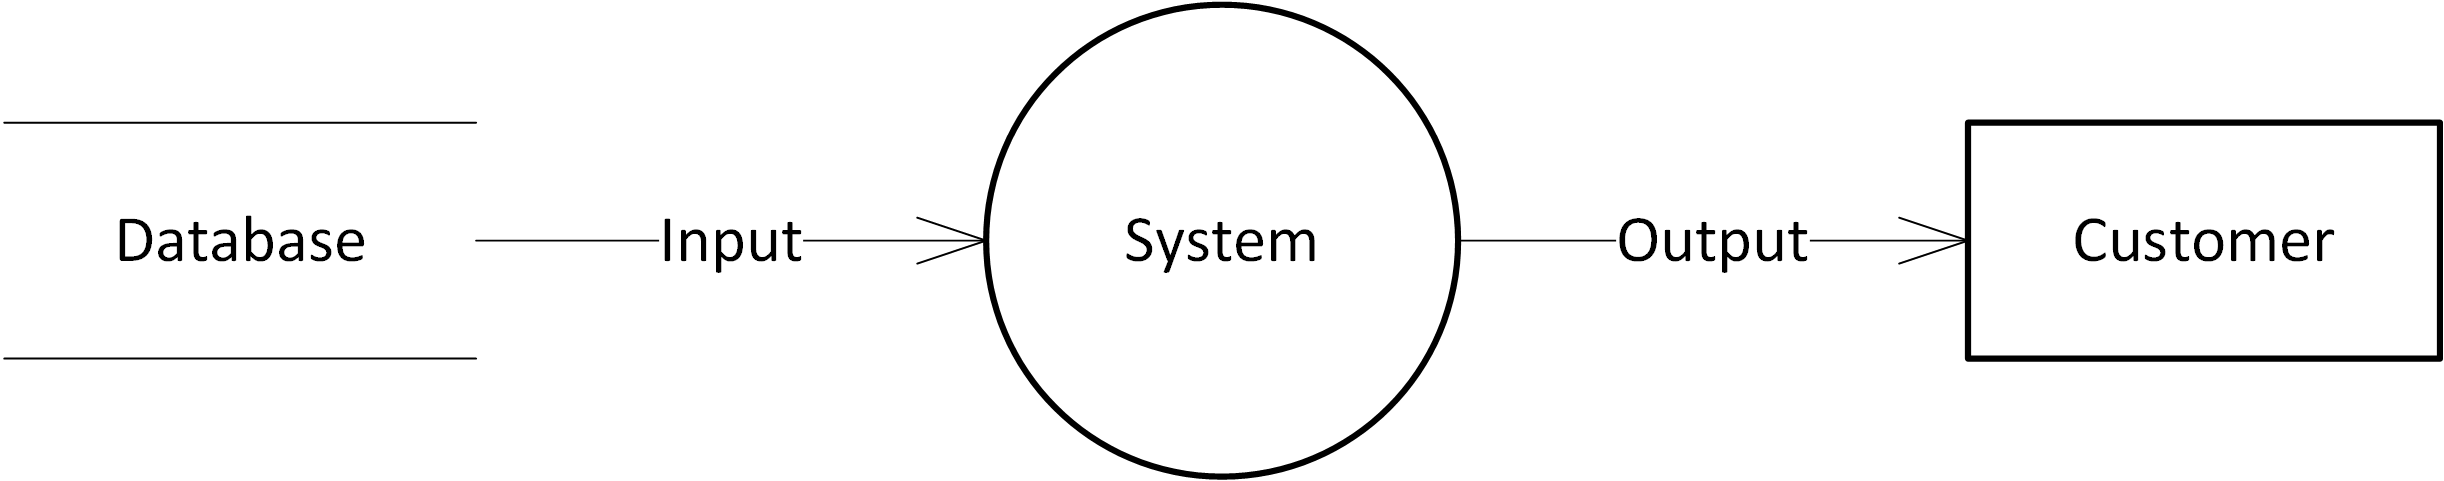
\includegraphics[width=0.8\textwidth]{images/datenflussdiagramm.png}
	\caption{Beispiel für ein Datenflussdiagramm}
	\label{img:datenflussdiagramm}
\end{figure}

\section{Informationsflussanalyse}
\label{sec:datenflussanalyse}
Die Modelle, die im Verlauf der Bachelorarbeit entstehen, sollen später als Eingabe für Datenflussanalysen dienen. Deshalb sind Arbeiten relevant, die sich mit Datenflussanalysen beschäftigen. Daraus können Anforderungen abgeleitet werden, die für die Modellierung benötigt werden. Im Folgenden sollen solche Arbeiten betrachtet werden. \par
Eine dieser Grundlagenarbeiten ist das Buch \textbf{Principles of Program Analysis} \cite{Basili1984}. In dieser Arbeit werden Datenflussanalysen auf Implementierungsebene beschrieben. Das heißt, dass um die Analyse ausführen zu können, eine Implementierung des Systems vorhanden sein muss. Die Datenflussanalyse wird mithilfe von Constant-Propagation, formuliert. Damit ist gemeint, dass konstante Ausdrücke zur Kompilierzeit ausgewertet werden. Ein Beispiel dafür ist in \autoref{img:constant_propagation} abgebildet. Dort werden die Kontrollkonstrukte statisch, zur Kompilierzeit, ausgewertet. 

\begin{figure}[h]
	\centering
  	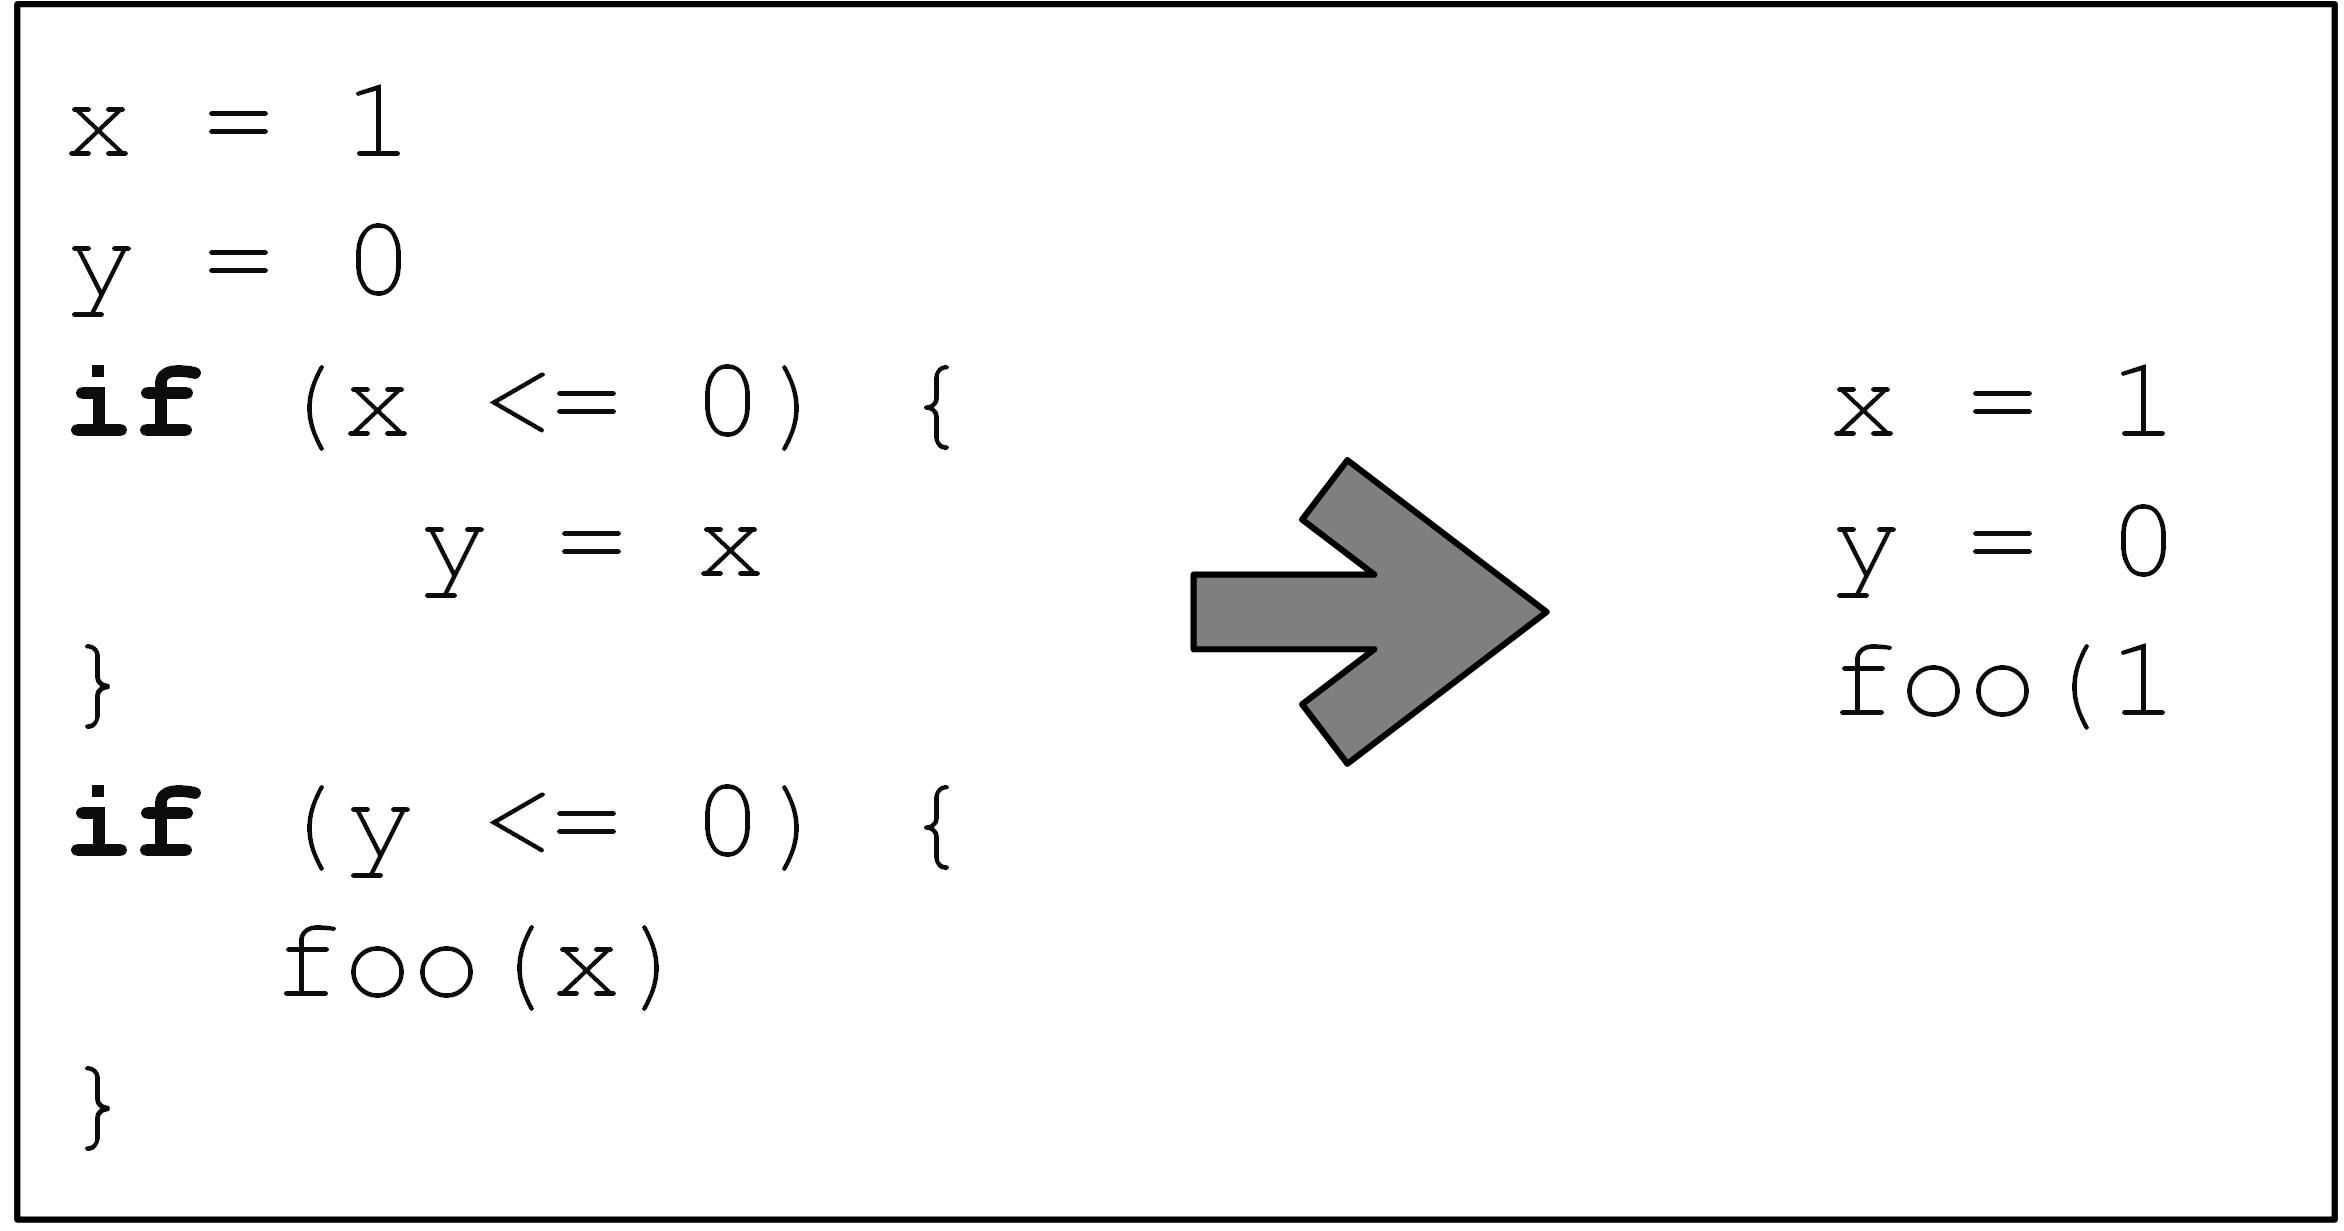
\includegraphics[width=0.7\textwidth]{images/cfg_code.png}
	\caption{Beispiel für Constant-Propagation}
	\label{img:constant_propagation}
\end{figure}

Der Ausgangspunkt für die Analyse ist dabei der \gls{cfg}. Ein \gls{cfg} besteht aus:
\begin{itemize}
\item Einer Menge von Knoten, die Instruktionen darstellen.
\item Einem Wurzelknoten, mit dem die Ausführung beginnt.
\item Einer Menge von gerichteter Kanten, die mögliche Programmabläufe darstellen.
\end{itemize}
In \autoref{img:cfg} ist der \gls{cfg} für das Beispiel aus \autoref{img:constant_propagation} abgebildet. Dabei werden in die Knoten eine oder mehrere Anweisungen des Codes eingetragen. Mit diesem \gls{cfg} kann im Anschluss eine Datenflussanalyse durchgeführt werden. \par
\begin{figure}[h]
	\centering
  	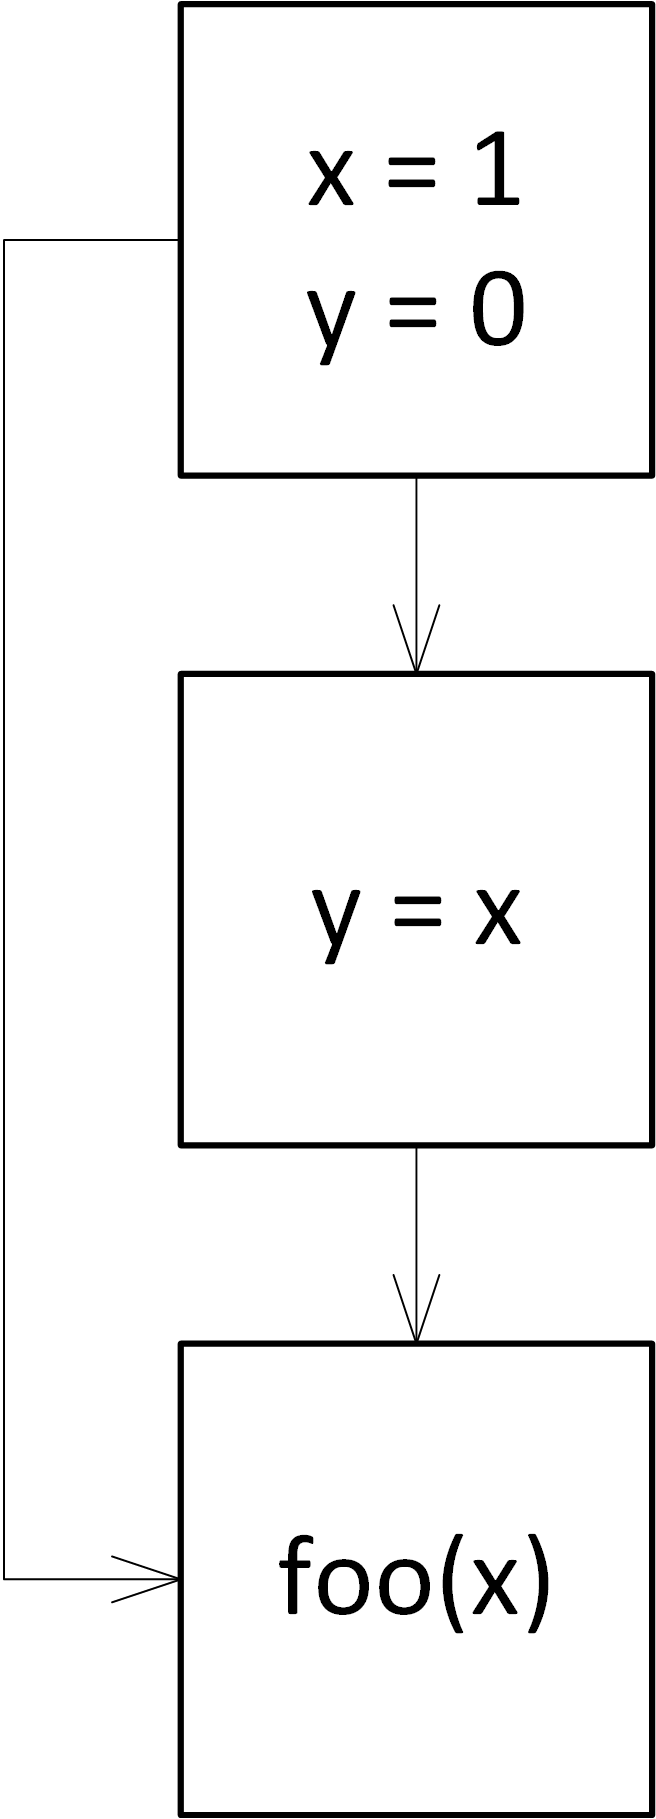
\includegraphics[width=0.16\textwidth]{images/cfg.png}
	\caption{Beispiel eines CFG, für das Beispiel aus \autoref{img:constant_propagation}}
	\label{img:cfg}
\end{figure}
Diese Analyse arbeitet jedoch nicht auf Datenflüssen, sondern leitet diese aus dem Kontrollfluss ab. Außerdem setzt die Analyse eine fertige Implementierung vorraus. In dieser Bachelorarbeit sollen Datenflüsse auf Architekturebene betrachtet werden. Dabei soll die Analyse direkt auf diesen Datenflüssen arbeiten und diese nicht aus dem Kontrollfluss ableiten. Deshalb soll im Weiteren nicht näher auf diese Arbeit eingegangen werden. \par 
In der Arbeit von Jürjens et al. \cite{Jurjens2005} wurde \textbf{UMLsec} vorgestellt. Dabei handelt es sich um eine Erweiterung für UML. \textbf{UMLsec} definiert 21 Stereotypen, die UML um Sicherheitseigenschaften erweitern. Ein Beispiel für einen Stereotypen, ist \texttt{Encrypted}. Mit diesem Stereotypen kann eine verschlüsselte Verbindung modelliert werden. Eine Sicherheitsanalyse kann im Anschluss mithilfe eines definierten Angreifers prüfen, ob das System sicher ist. Auch hier werden Datenflüsse nicht direkt verwendet, sondern aus dem Kontrollfluss abgeleitet. Da die Erweiterung für UML konzipiert ist und im Vordergrund der Arbeit die Sicherheit eines Systems und nicht der Datenfluss steht, wird sie im weiteren Verlauf der Bachelorarbeit nicht weiter betrachtet. \par
Eine Arbeit, die sich mit Datenflüsse auf Architekturebene befasst, ist die bereits in \autoref{sec:palladioerweiterungen} vorgestellte Arbeit \textbf{Model-Driven Specification and Analysis of Confidentiality in Component-Based Systems} \cite{Kramera}. Sie erweitert das \gls{pcm} um Datenflüsse und eine Vertraulichkeitsanalyse. Die Arbeit basiert auf dem Poster \textbf{Specification and Verification of Confidentiality in Component-Based Systems} \cite{Kramer}. Datenflüsse werden aber nicht innerhalb der Komponenten betrachtet. Außerdem werden Datenflüsse aus dem Kontrollfluss abgeleitet. Stattdessen werden Anforderungen für das Verhalten der Datenflüsse spezifiziert und anschließend überprüft. Die Prüfung der Komponente erfolgt zur Implementierungszeit auf Basis des Quelltexts. Die Arbeit beschreibt außerdem eine Vertraulichkeitsanalyse für Palladio. Diese Analyse prüft die Vertraulichkeit in komponentenbasierten Systemen. Für die Analyse müssen Eingabe und Ausgabe eines Systems spezifiziert werden, sowie Zugriffsspezifikation für Hardware und Kommunikationsverbindungen. Mithilfe dieser Informationen und einem Angreifer Modell, wird eine Architektur- und Code-Analyse durchgeführt. Nach Durchführung der Analyse werden Designfehler, Datenlecks und Verstöße gegen die Spezifikation angezeigt. Die Vertraulichkeitsanalyse hält sich ebenfalls an die Definition von Vertraulichkeit nach Eckert \cite{Eckert2013}. \par
In allen vorgestellten Arbeiten werden Eigenschaften für Daten festgemacht. Jedoch werden die Datenflüsse aus Kontrollflüssen abgeleitet. In dieser Bachelorarbeit sollen Daten und Datenflüsse als Objekte erster Klasse eingeführt werden. Für die Validierung soll jedoch die Vertraulichkeitsanalyse aus \cite{Kramer2012} verwendet werden, da diese bereits eine funktionierende Vertraulichkeitsanalyse für Palladio anbietet.

\section{Erweiterung des PCM}
Die Erweiterung des PCMs erfolgt durch die Erweiterung seines Meta-Modells. Dazu wurde von Strittmatter et al. \cite{Strittmatter} ein Ansatz entwickelt, bei dem die zu modellierenden Informationen in Gruppen eingeteilt werden. Das Meta-Modell wird in Schichten eingeteilt, die jeweils eine Gruppe abbilden. Schichten referenzieren sich gegenseitig. Dies führt zu einer modularen, flexiblen und erweiterbaren Struktur, die die Koexistenz von verschiedenen Qualitätsattributen und -analysen ermöglicht. Das Meta-Modell ist in die folgenden vier Schichten unterteilt:
\begin{itemize}
\item Die \textbf{Paradigm}-Schicht ist die Basisschicht. Sie legt den Grundstein für die Modellierungssprache, indem sie die Struktur, aber keine Semantik bereitstellt.
\item Die Semantik für die abstrakte Struktur der Sprache liefert die \textbf{Domain}-Schicht.
\item In der \textbf{Quality}-Schicht werden Qualitätseigenschaften für bestimmte Bereiche hinzugefügt.
\item Schließlich bietet die \textbf{Analysis}-Schicht Module für die Eingabe, Ausgabe und den internen Zustand. Außerdem gibt es Konfigurationsoptionen für Analysen.
\end{itemize}
Diese Arbeit wird für die Modellierung in \autoref{ch:modellierung} verwendet.

%% LaTeX2e class for student theses
%% sections/content.tex
%% 
%% Karlsruhe Institute of Technology
%% Institute for Program Structures and Data Organization
%% Chair for Software Design and Quality (SDQ)
%%
%% Dr.-Ing. Erik Burger
%% burger@kit.edu
%%
%% Version 1.1, 2014-11-21

\chapter{Modellierung}
\label{ch:modellierung}

Während der Bachelorarbeit wurde ein Meta-Modell zur Darstellung von Daten und Datenflüssen, in Palladio, erstellt. Dabei wurde nach dem Prozess von Völter und Stahl vorgegangen \cite{StahlThomasVoelterMarkus2006}. Dieser beschreibt das Vorgehen für die Entwicklung eines Meta-Modells.
%Eine Übersicht findet sich in Abb. [ref]. \todo{Abb für den Prozess}
Der Prozess besteht aus mehreren Schritten. Zunächst findet eine Domänenanalyse statt. Sie besteht aus einer Anforderungserhebung (\autoref{sec:anforderungserhebung}) und anschließender Meta-Modell-Bildung (ab \autoref{sec:metabildung}). Nach der Domänenanalyse folgt die Erstellung eines Referenzmodells (\autoref{sec:travelplanner}). Dabei handelt es sich um eine Instanz des Meta-Modells, aus dem ersten Schritt. Als nächstes wird das Programmiermodell dokumentiert. Das Programmiermodell erklärt, wie eine Anwendung implementiert werden kann, die auf dem Meta-Model basiert. In der Bachelorarbeit fällt das Programmiermodell weg, da kein Quelltext erzeugt wird und auch sonst das Ergebnis der Modellierung nicht mehr weiter, in einer anderen Form, bearbeitet werden muss. Im nächsten Schritt wird eine Transformation (\autoref{sec:implementierung}) durchgeführt. Dieser Schritt dient dazu, ein gegebenes Anwendungsmodell automatisch in eine Implementierung oder einen Rahmen zu überführen. Schließlich soll zu dem Meta-Modell noch ein Editor erstellt werden. Ein Editor stand nicht im Fokus der Bachelorarbeit und wurde deshalb nicht realisiert. Allgemein kann das Modell im automatisch erzeugten Editor der Eclipse IDE editiert werden. \par
Auf die Anforderungserhebung, sowie das Meta-Modell wird in den folgenden Abschnitten genauer eingegangen. Das Referenzmodell und die Transformation werden in der Validierung in \autoref{ch:validierung} erläutert.


\section{Anforderungserhebung}
\label{sec:anforderungserhebung}
Bei der Anforderungserhebung wurde das Meta-Modell aus der Arbeit \textbf{Model-Driven Specification and Analysis of Confidentiality in Component-Based Systems} \cite{Kramera} untersucht. Dabei wurde nach Elementen gesucht, die zum Ableiten des vertraulichkeitsrelevanten Verhaltens einer Komponente benötigt werden, jedoch noch nicht vorhanden sind und welche man generisch in Datenflüssen ausdrücken kann. Dazu wurde die Vertraulichkeitsanalyse aus \autoref{sec:datenflussanalyse} untersucht. Für die Analyse müssen Eingabe und Ausgabe des zu untersuchenden Systems spezifiziert werden. Außerdem können Zugriffsspezifikationen für Hardware und Kommunikationsverbindungen spezifiziert werden. Um dies spezifizieren zu können, wurde ein Annotationsmodell eingeführt. Bei einem Annotationsmodell handelt es sich um ein strukturiertes Modell von Annotationen. Die Annotationen können an Elemente im Komponenten-Repository- und Ressourcen-Umgebungs-Modell angehängt werden, um diese zu erweitern und zusätzliche Informationen zu liefern. Das Annotationsmodell wurde für die Bachelorarbeit nachmodelliert. Dabei wurde darauf geachtet, dass das Modell in Zukunft erweiterbar ist, z.B. zur Nutzung für neue oder andere Qualitätsanalysen. Mithilfe von Oberklassen wurde eine Schnittstelle geschaffen, die das ermöglicht. Außerdem sollte eine Gruppierung der Elemente möglich sein, z.B. je untersuchtem Qualitätsattribut. Dieses Verhalten wurde mithilfe von Containern sichergestellt. Das Modell wird in \autoref{sec:stereotypes} beschrieben. \par 
In der Arbeit \cite{Kramera} wird mithilfe von \texttt{DataSet}s die Eingabe und Ausgabe des Systems spezifiziert. Ein \texttt{DataSet} ist dabei eine Gruppierung von Daten, die in dem System verarbeitet werden. Eine Datenflussanalyse innerhalb von Komponenten ist nicht vorgesehen. Für die Komponente werden gewünschte Ergebnisse für die Eingabe und Ausgabe spezifiziert. Im Anschluss untersucht die Analyse, wie sich einzelne Parameter gegenseitig beeinflussen. Mithilfe der Modellierung dieser Bachelorarbeit soll aber auch der Datenfluss innerhalb von Komponenten nachvollzogen werden. Es sollen außerdem nicht direkt Parameter, sondern Daten betrachtet werden. Das heißt, dass es möglich sein muss angeben zu können welche Daten sich innerhalb von Komponenten beeinflussen. Außerdem muss es möglich sein Daten Parametern zuordnen zu können. Dazu müssen zunächst Daten modelliert werden. Dabei handelt es sich nicht um individuelle Daten sondern um Datenklassen. Die Modellierung ist in \autoref{sec:data} beschrieben. Der Datenfluss der Daten innerhalb von Komponenten, soll mithilfe eines \gls{dfseff} modelliert werden. Bei diesem \gls{dfseff} soll nur die Eingabe spezifiziert werden. Das heißt, dass nur die \texttt{DataSet}s der Eingabe spezifiziert werden. Die Ausgabe wird aus der Modellierung des \gls{dfseff} abgeleitet. Aktionen die ein \gls{dfseff} unterstützt sind Aufrufe an externe Dienste, das Kombinieren von mehreren Datenklassen zu einer neuen und das Erstellen einer neuen Datenklasse. Zu diesen Aktionen gehört auch die Fähigkeit Daten und Parameter zu verknüpfen. In \autoref{sec:paket:dfseff} wird der \gls{dfseff} beschrieben. Außerdem soll die Eingabe eines Benutzers des Systems, mithilfe von Datenflüssen untersuchbar sein. Auch hier soll nur die Eingabe spezifiziert werden. Wohin die Daten fließen, wird auch hier aus der Modellierung abgeleitet. Eine Beschreibung dieses Modells befindet sich in \autoref{sec:paket:usage}. \par
Die Meta-Modell-Bildung orientiert sich an der Arbeit von Strittmatter et. al. \cite{Strittmatter}. Dabei wurde die \textbf{Quality}-Schicht erweitert, da dort Qualitätseigenschaften spezifiziert werden können. Außerdem wurde die \textbf{Domain}-Schicht um weitere Attribute und Qualitätseigenschaften erweitert. Die \textbf{Analysis}-Schicht wurde für die Validierung prototypisch erweitert. Allerdings ist die Analyse kein Kernbeitrag dieser Bachelorarbeit. Die Arbeit zur Meta-Modell-Erweiterung wurde in \autoref{ch:verwandteArbeiten} beschrieben. \par
Als nächstes wurde untersucht, welche bestehenden Palladio-Elemente wiederverwenden werden können und welche neu modelliert werden müssen. Dabei kann die Wiederverwendung auf Meta-Modell- und Modell-Ebene statt finden. Bei ersterem, wird bei der Erstellung des Datenfluss-Meta-Modells auf bestehenden Meta-Modell-Elementen des \gls{pcm} aufgebaut. Beim zweiten, kann der Architekt seine bestehenden \gls{pcm}-Modelle um Datenflüsse erweitern. Die Vorteile bei der Wiederverwendung von \gls{pcm}-Meta-Modell-Elementen sind, dass der Meta-Modellierer weniger Arbeit hat, da er auf bestehenden Elemente aufbaut und diese nicht nochmal modellieren muss. Der Benutzer hat den Vorteil, dass auch er bereits erstellte Elemente nicht nochmal modellieren muss und seine Modelle nur um Datenflüsse erweitern kann. Außerdem muss er keine neuen Elemente lernen. Nachteile sind jedoch, dass die Semantik der existierenden Elemente nicht zur angepeilten Semantik der neuen Elemente passen muss. Das äußert sich z.B. dadurch, dass Referenzen zu Elementen existieren, die für den Anwendungsfall irrelevant sind. Eine mögliche Referenz ist der \gls{rdseff}. Dies kann zu einem Problem führen, da in dieser Bachelorarbeit, unter anderem ein \gls{seff} modelliert werden soll, mit dem Datenflüsse modellierbar sind. Bei der Wiederverwendung der Elemente, die den \gls{rdseff} referenzieren, wird der \gls{dfseff} abhängig vom \gls{rdseff}. Für den Benutzer entsteht dadurch auch eine unklare Semantik, da dieser nicht weiß, welche Eigenschaften er angeben muss, um sinnvolle Ergebnisse zu erhalten. Außerdem gibt es Elemente die zwar unabhängig vom RDSEFF sind, aber Attribute enthalten, die für den Anwendungsfall unbrauchbar sind. Auch hier entsteht für den Benutzer eine unklare Semantik. Außerdem können Änderungen keine Auswirkung haben, da die angegebenen Eigenschaften nicht verwendet werden. Eine Wiederverwendung wird deshalb nur durchgeführt, wenn die Semantik übernommen oder sinnvoll erweitert werden kann, z.B. wenn alle Referenzen in beiden Kontexten sinnvoll sind. \par
Die Ergebnisse der Meta-Modell-Bildung werden in den folgenden Abschnitten präsentiert. 

\section{Übersicht der Pakete}
\label{sec:metabildung}
Das Meta-Modell besteht aus den in \autoref{img:pakete} gezeigten Paketen. Die Pakete orientieren sich an den in Palladio verwendeten Sichten aus \autoref{ch:pcm}. \par
Das Paket \texttt{Container-Stereotypes} erweitert das Ressourcen-Umgebungs-Modell. Für die Erweiterung ist der Softwareverteilungsexperte zuständig. Es enthält Eigenschaften, die an einen Resource-Container oder eine Linking-Resource in Palladio angehängt werden können. Dabei handelt es sich bei einer Linking-Resource um einen Verbindungskanal. Bei einem Resource-Container handelt es sich um eine Hardware-Ressource. Die Elemente sind in \autoref{sec:stereotypes} genauer beschrieben. \par
Das Paket \texttt{DFSEFF} erweitert das Komponenten-Repository-Modell. Es ist für die Modellierung eines \gls{seff}s zuständig, mit dem es möglich ist, den Datenfluss innerhalb einer Komponente zu modellieren. Die Informationen, die für die Modellierung benötigt werden, werden vom Komponentenentwickler bereitgestellt. In \autoref{sec:paket:dfseff} wird die Erweiterung genauer beschrieben. \par
Das Paket \texttt{Data} erweitert (momentan) das Repository-Modell und das Nutzungsmodell. Die Informationen werden dabei vom Komponentenentwickler und dem Domänenexperten bereitgestellt. In dem Paket werden Daten modelliert, die in einem System verwendet werden. Dabei handelt es sich nicht um individuelle Daten, sondern um Datenklassen. Eine genaue Beschreibung befindet sich in \autoref{sec:data}. \par
Schließlich erweitert das Paket \texttt{Usage} das Nutzungsmodell. Alle Elemente die für die Modellierung des Datenflusses für das Nutzungsmodell in Palladio benötigt werden, befinden sich darin. Der Domänenexperte ist für die Modellierung und Erweiterung zuständig. Die Erweiterung wird in \autoref{sec:paket:usage} genauer beschrieben. \par
%Die hier und im Folgenden vorgestellte Erweiterung ist als Annotationsmodell konzipiert.

\begin{figure}[htp]
	\centering
  	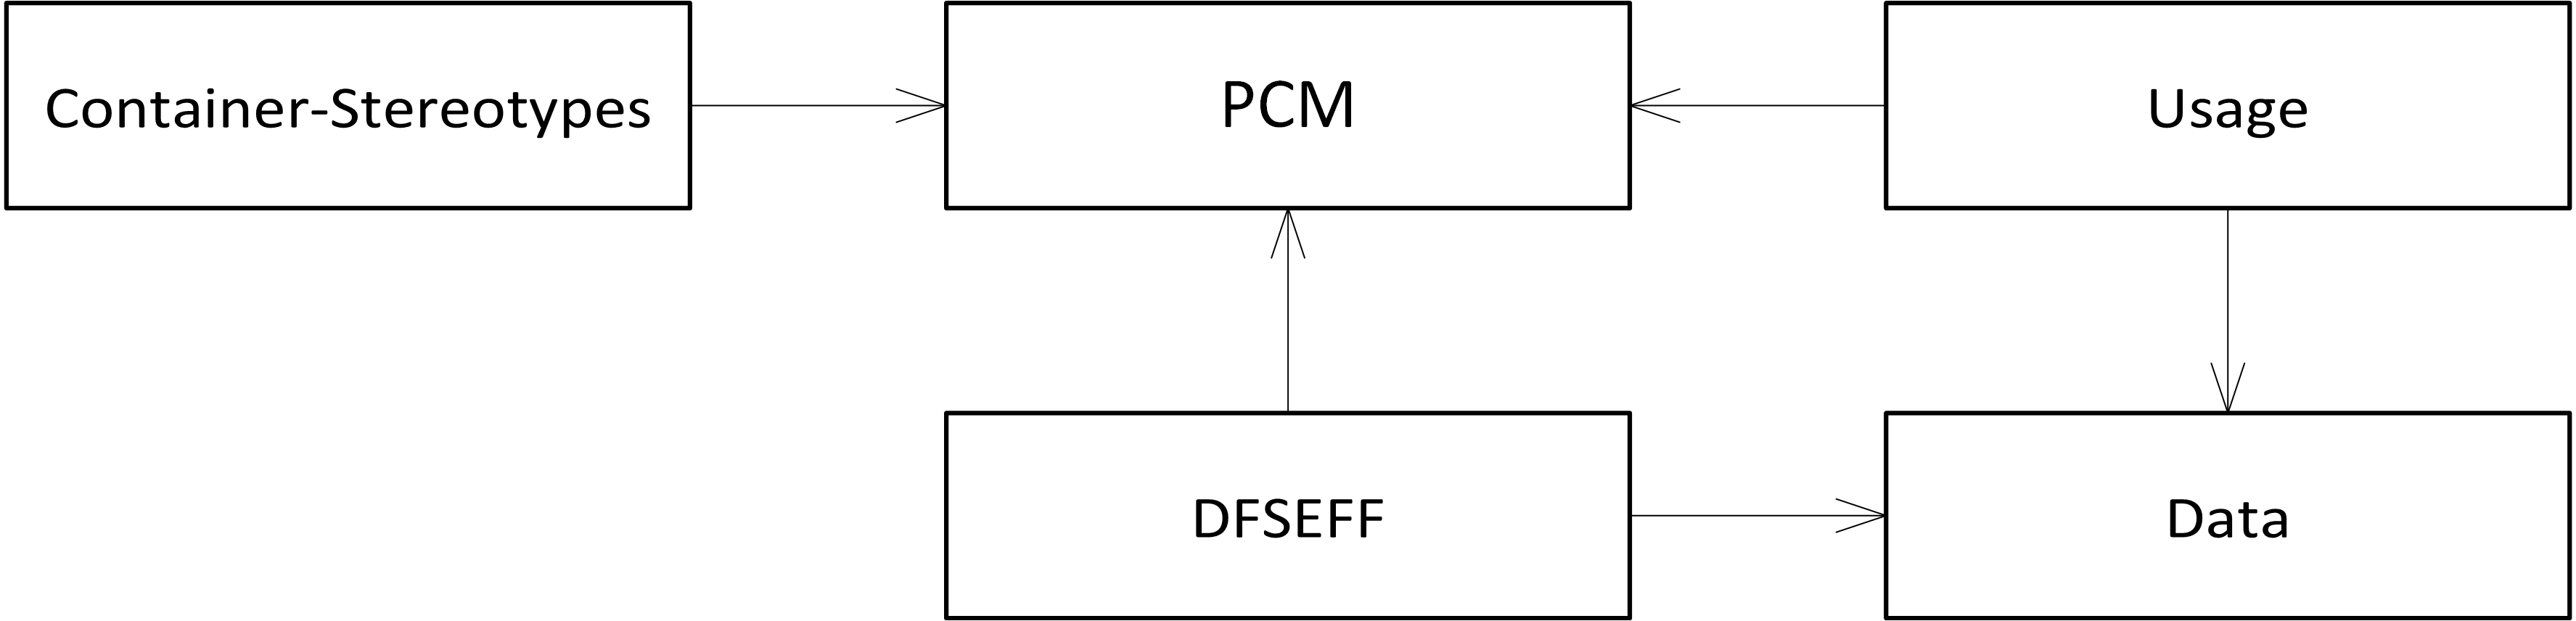
\includegraphics[width=1\textwidth]{images/pakete.png}
	\caption{Übersicht der Pakete der Meta-Modell-Erweiterung}
	\label{img:pakete}
\end{figure}

\section{Beispielszenario}
\label{sec:szenario}
Um die im Folgenden beschriebenen Modellierung besser zu veranschaulichen, soll an dieser Stelle ein Szenario beschrieben werden, in das die einzelnen Pakete und Elemente eingeordnet werden können. In \autoref{img:szenario} ist das Szenario abgebildet. In diesem Szenario gibt es einen Laden, der ein Warenlager hat. In diesem Warenlager befinden sich Produkte. Der Laden besteht nur aus dem Besitzer und nur dieser hat Zugang zu dem Warenlager. Wenn ein Kunde in den Laden kommt richtet er seine Kaufbegehren an den Ladenbesitzer und dieser verkauft ihm je nach Verfügbarkeit das gewünschte Produkt. Für diesen Kaufvorgang benötigt der Ladenbesitzer die Kreditkarte des Kunden. Der Geldbetrag wird mithilfe eines Kreditkartenlesegeräts bei der Bank des Kunden eingefordert. Das Kreditkartenlesegerät ist über das Internet mit der Bank verbunden.

\begin{figure}[h]
	\centering
  	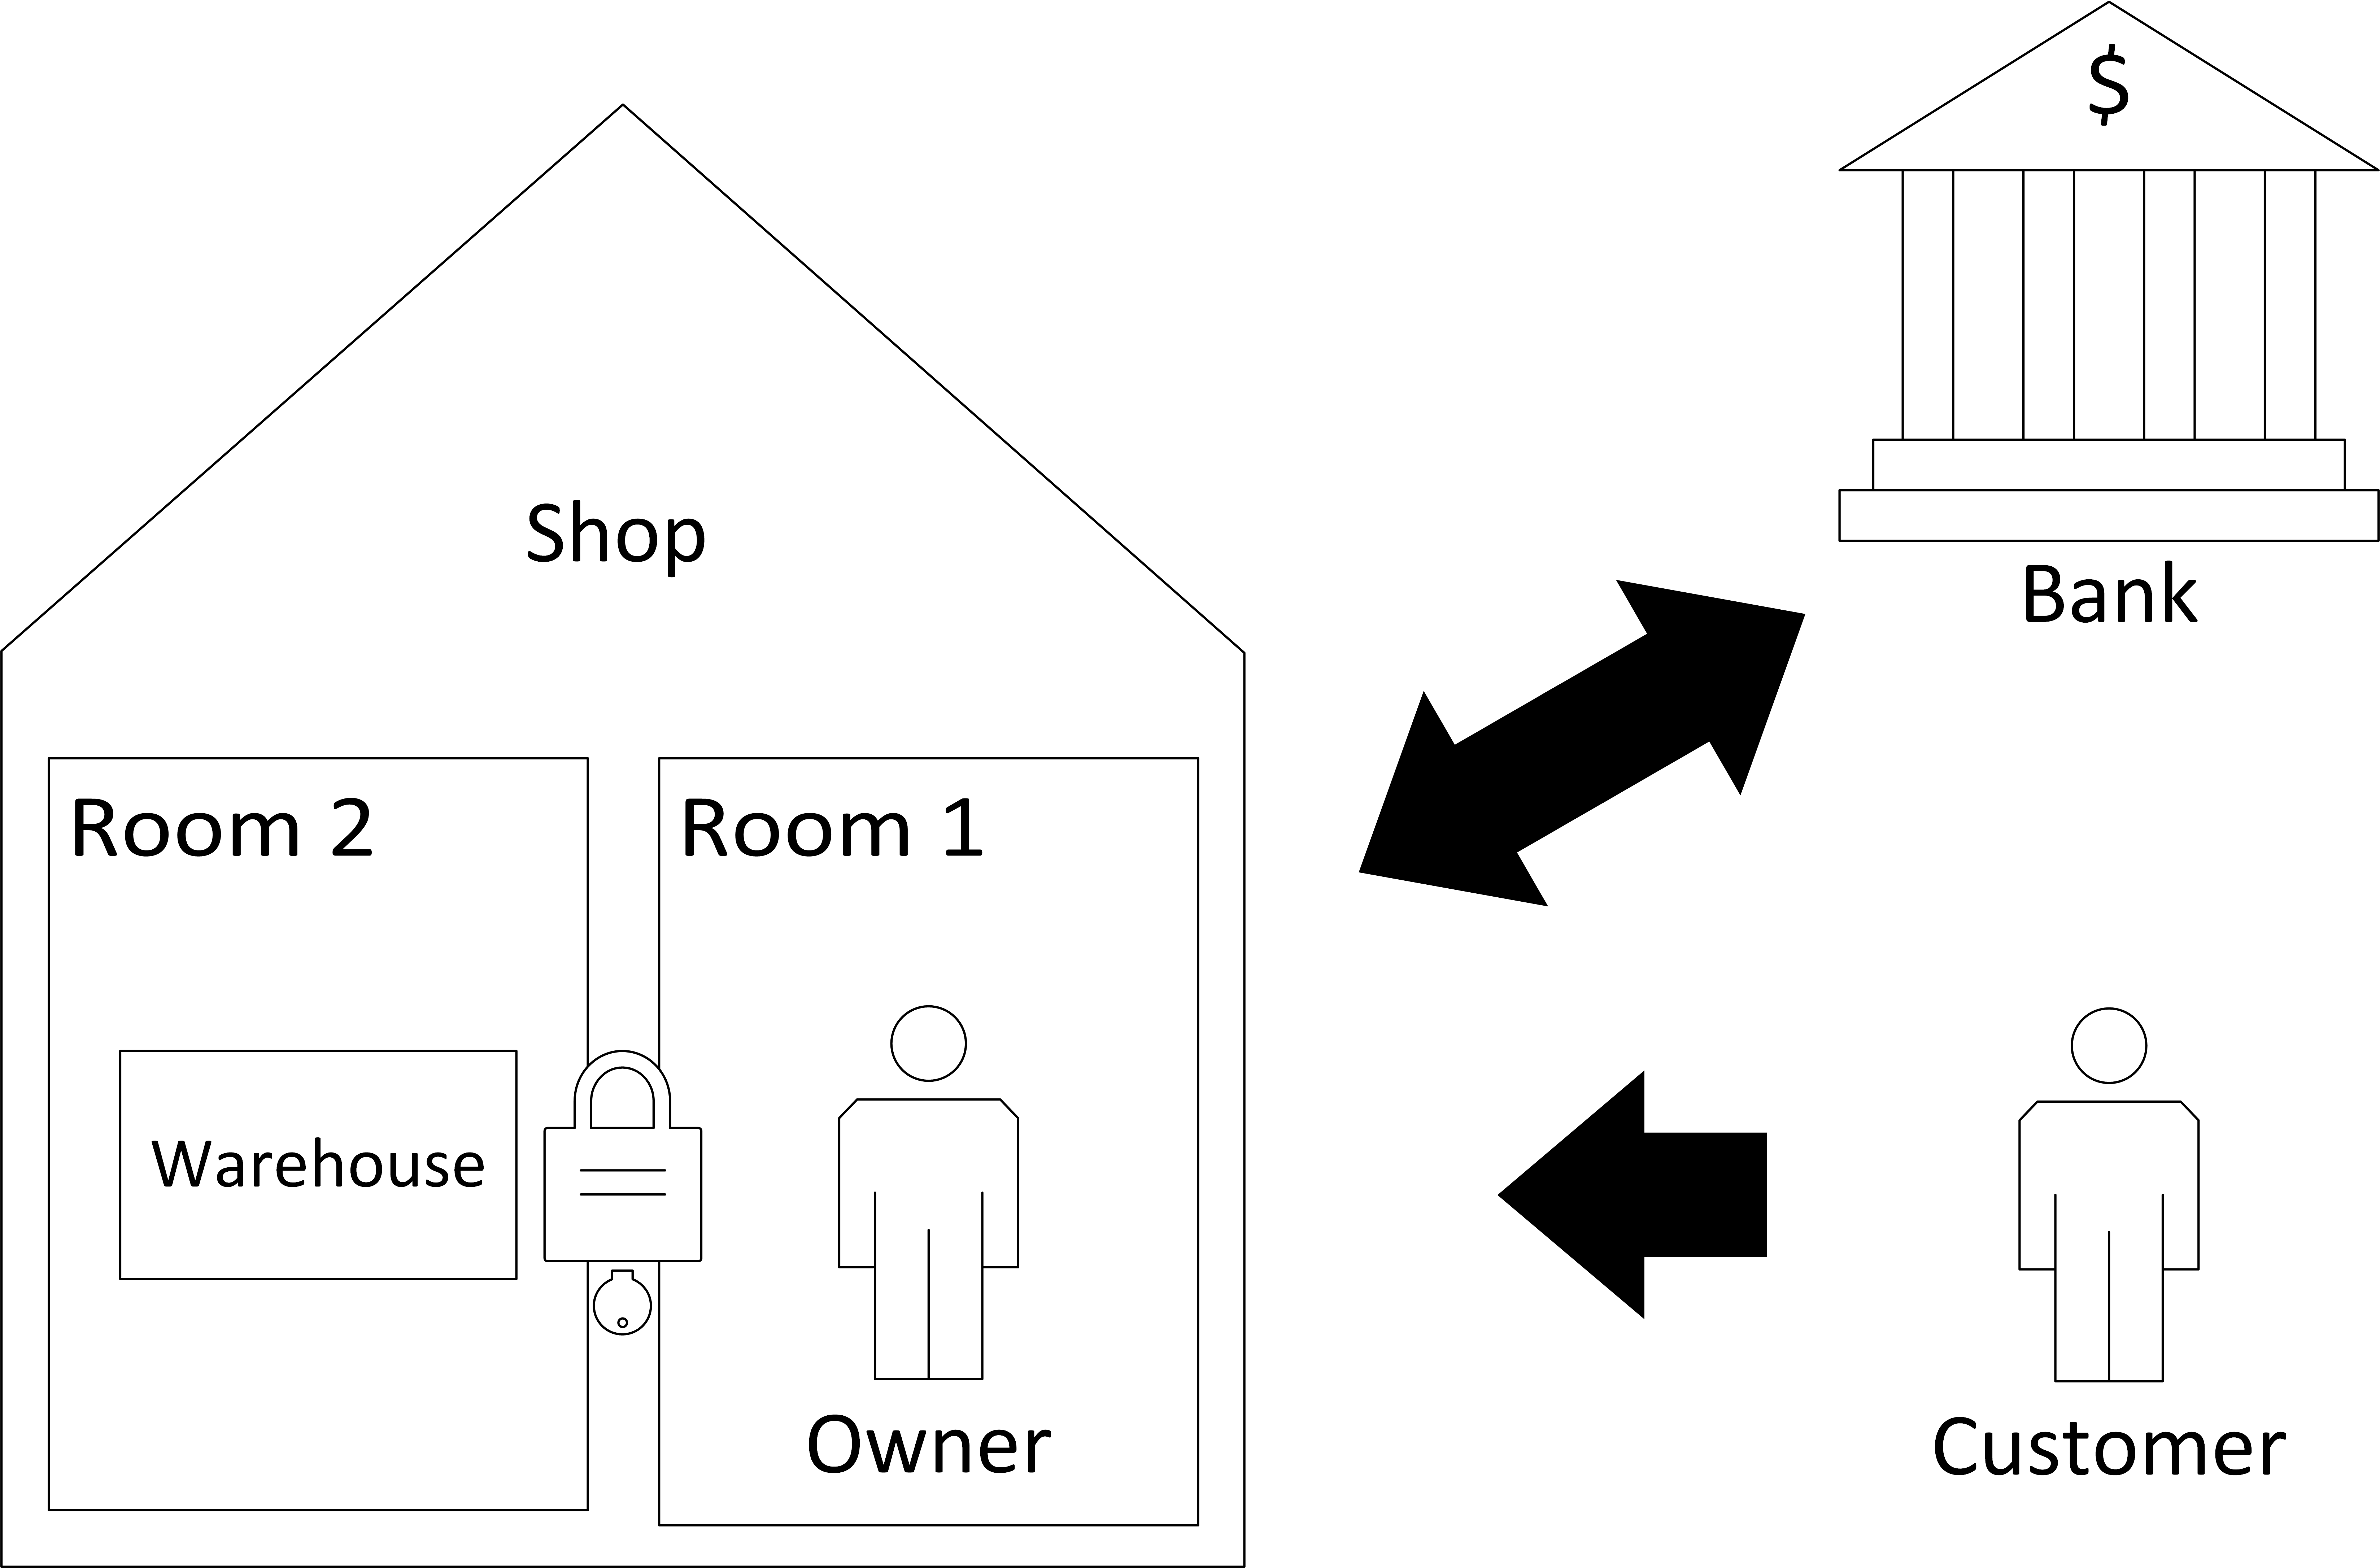
\includegraphics[width=0.6\textwidth]{images/szenario.png}
	\caption{Das Laden-Beispiel-Szenario}
	\label{img:szenario}
\end{figure}

Der Kaufvorgang ist in \autoref{img:szenario:seq} abgebildet. Der Kunde signalisiert dem Besitzer des Ladens, welches Produkt er haben möchte. Der Besitzer prüft nun im Warenlager, ob dieses Produkt vorhanden ist. Ist das der Fall, holt er es heraus und gibt es dem Kunden. Daraufhin bezahlt dieser mit seiner Kreditkarte. Dies ist nur der Basis-Kaufvorgang. Es gibt noch weitere Abläufe, die hier nicht beschrieben werden, wie z.B., wenn das Produkt nicht vorhanden ist.

\begin{figure}[h]
	\centering
  	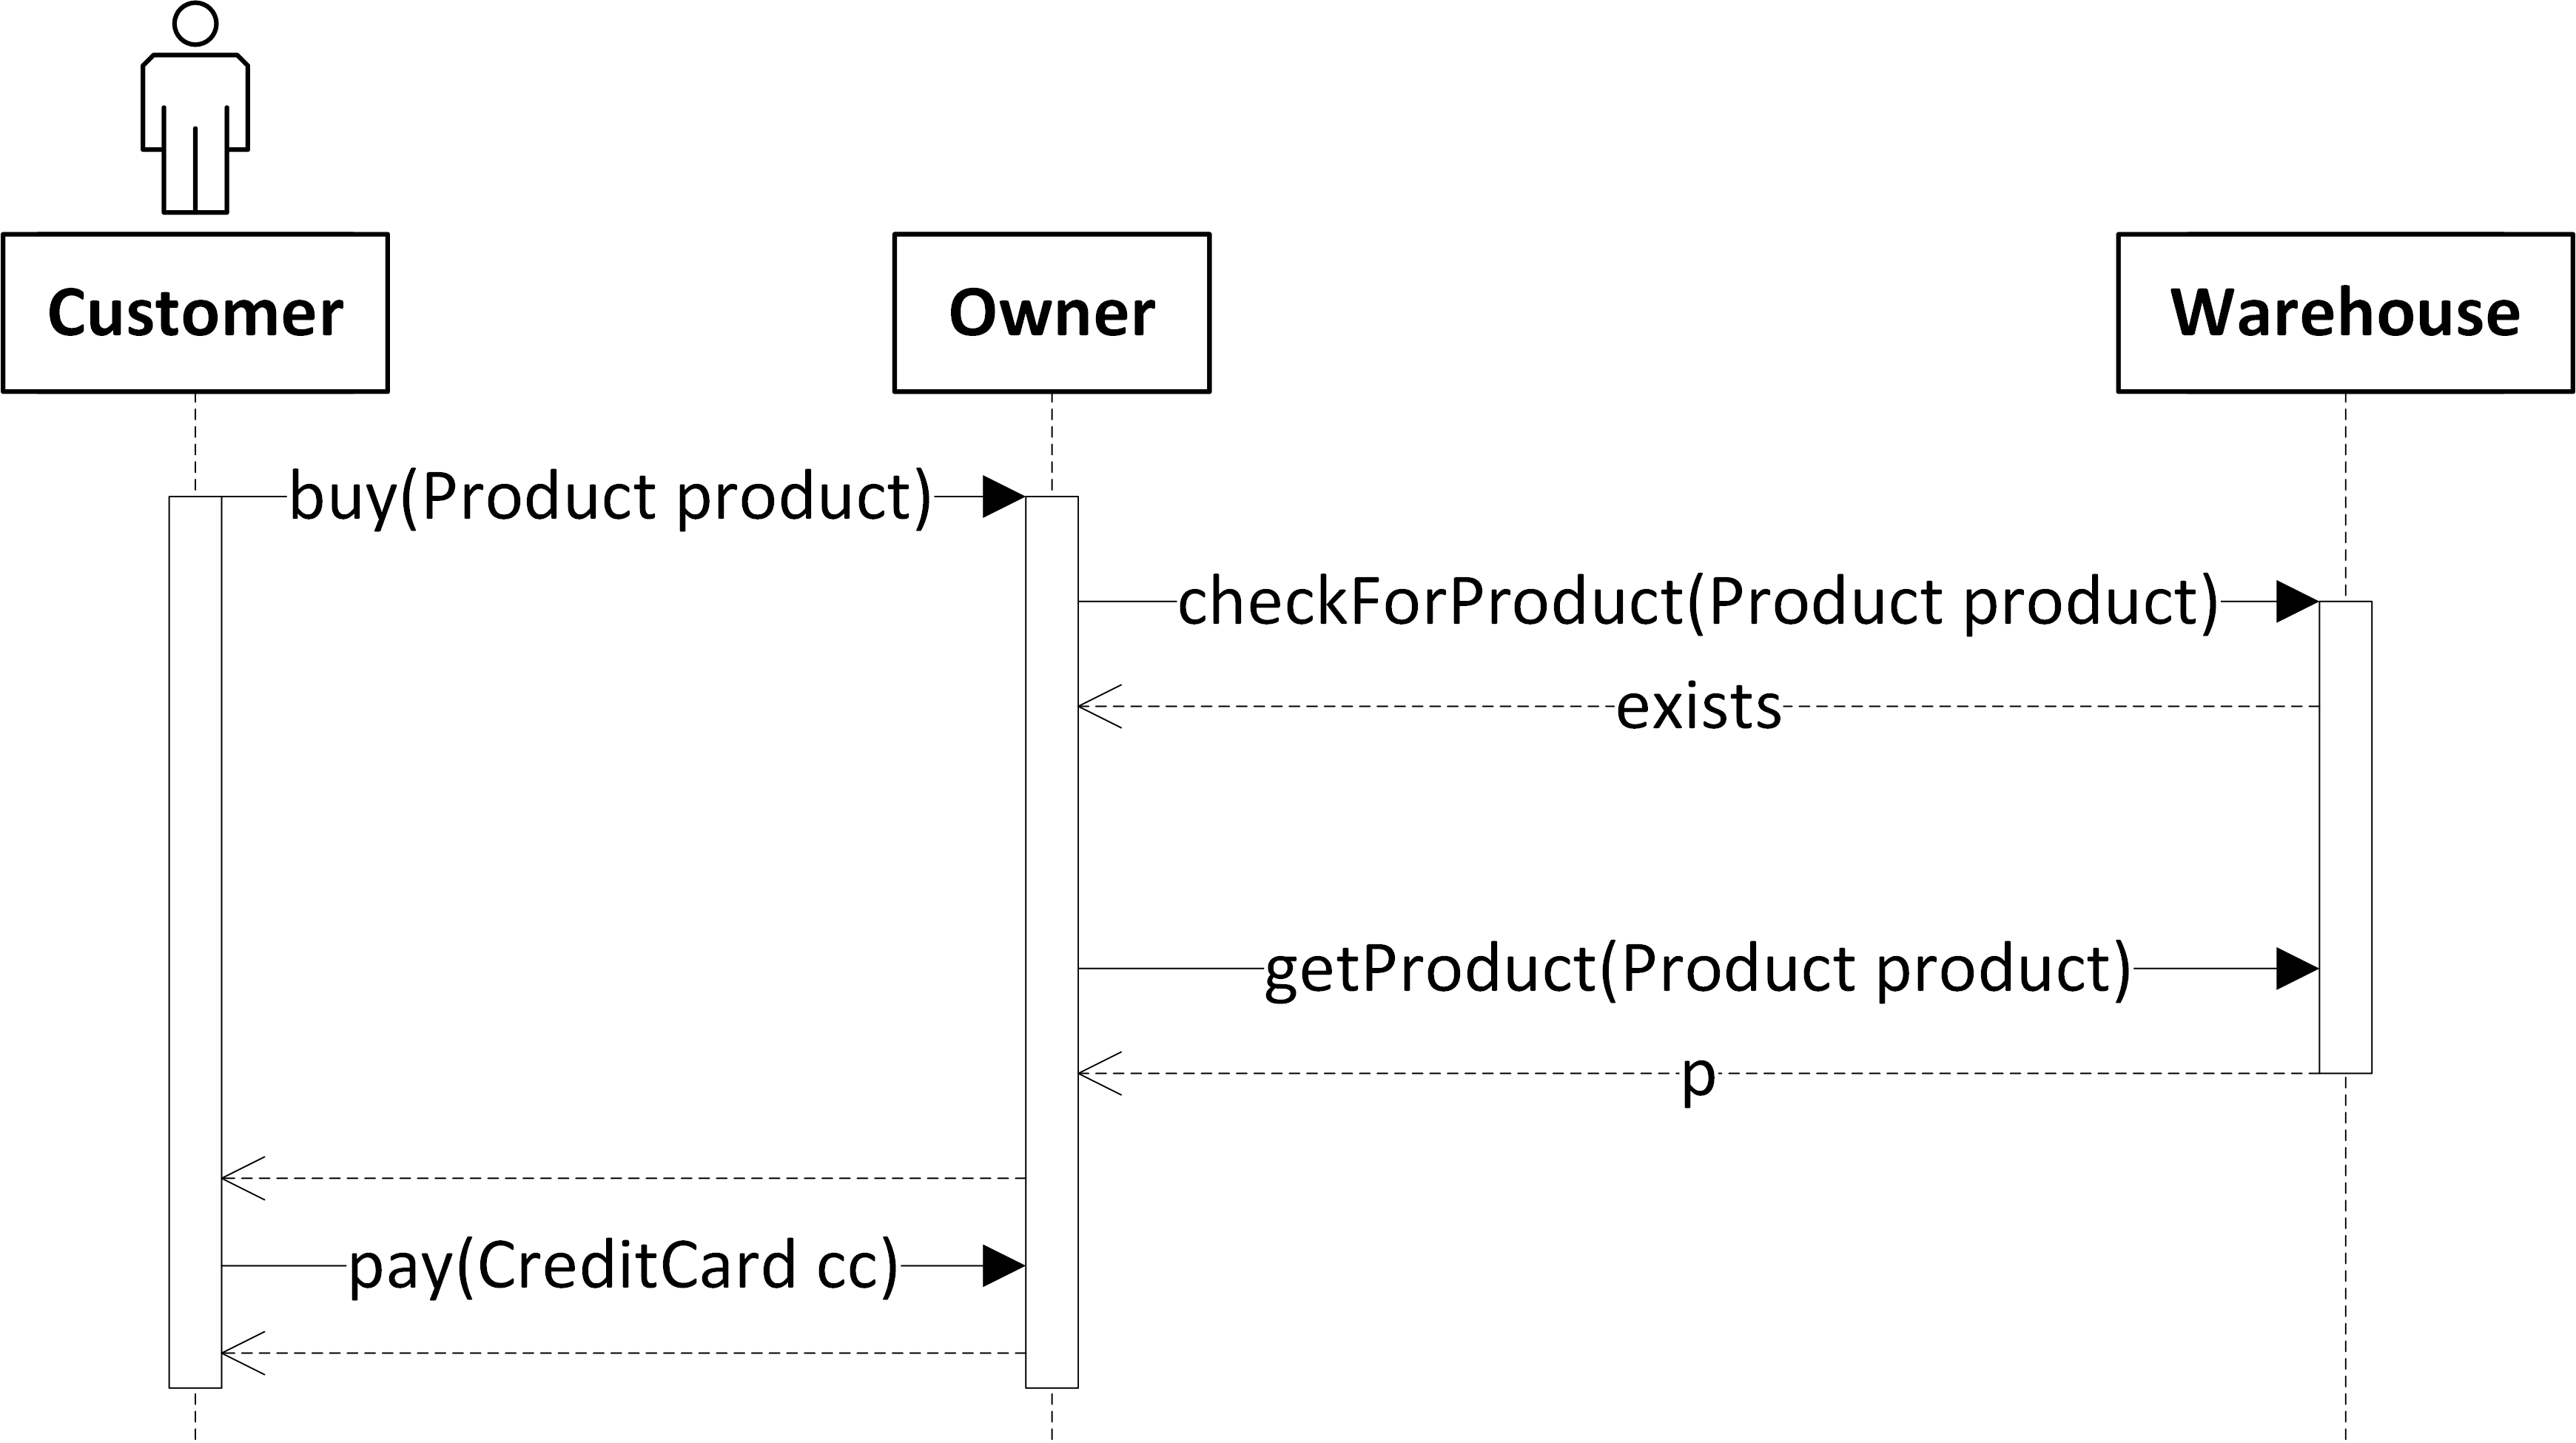
\includegraphics[width=1\textwidth]{images/szenario_seq.png}
	\caption{Der Ablauf eines Basis-Kaufvorgangs im Laden}
	\label{img:szenario:seq}
\end{figure}

\section{Software-Verteilungsexperte}
\label{sec:stereotypes}
Im folgenden wird die Erweiterung des Ressourcen-Umgebungs-Modells vorgestellt. Mithilfe dieser Erweiterung lassen sich die Linking-Resource oder der Resource-Container um verschiedene Eigenschaften erweitern. Die hier beschriebenen Eigenschaften stammen aus \cite{Kramera}, um Vertraulichkeit auf Hardware-Ebene zu unterstützen. Die Eigenschaften werden vom Softwareverteilungsexperten erstellt und referenzieren Resource-Container und Linking-Resources im Execution-Environment-Modell. Eine Darstellung des Modells ist in \autoref{img:modell:stereotypes:übersicht} abgebildet. \par
Damit in Zukunft weitere Eigenschaften hinzugefügt werden können, haben diese eine gemeinsame Oberklasse. Dadurch ist Erweiterbarkeit möglich. Dabei haben die Eigenschaften des Resource-Containers und der Linking-Resources jeweils eine eigene Oberklasse. Außerdem erweitern die Eigenschaften nicht direkt den Resource-Container bzw. die Linking-Resource, sondern werden in einem Container-Element gesammelt und dieser verweist auf den jeweiligen Resource-Container, bzw. die jeweilige Linking-Resource. Dies hat außerdem den Vorteil, dass mehrere Container auf einen Resource-Container oder eine Linking-Resource verweisen können und somit Eigenschaften gruppiert werden können. Nicht benötigte Gruppen können dann bei Bedarf ein- oder ausgeblendet werden. \par
\begin{figure}[h]
	\centering
  	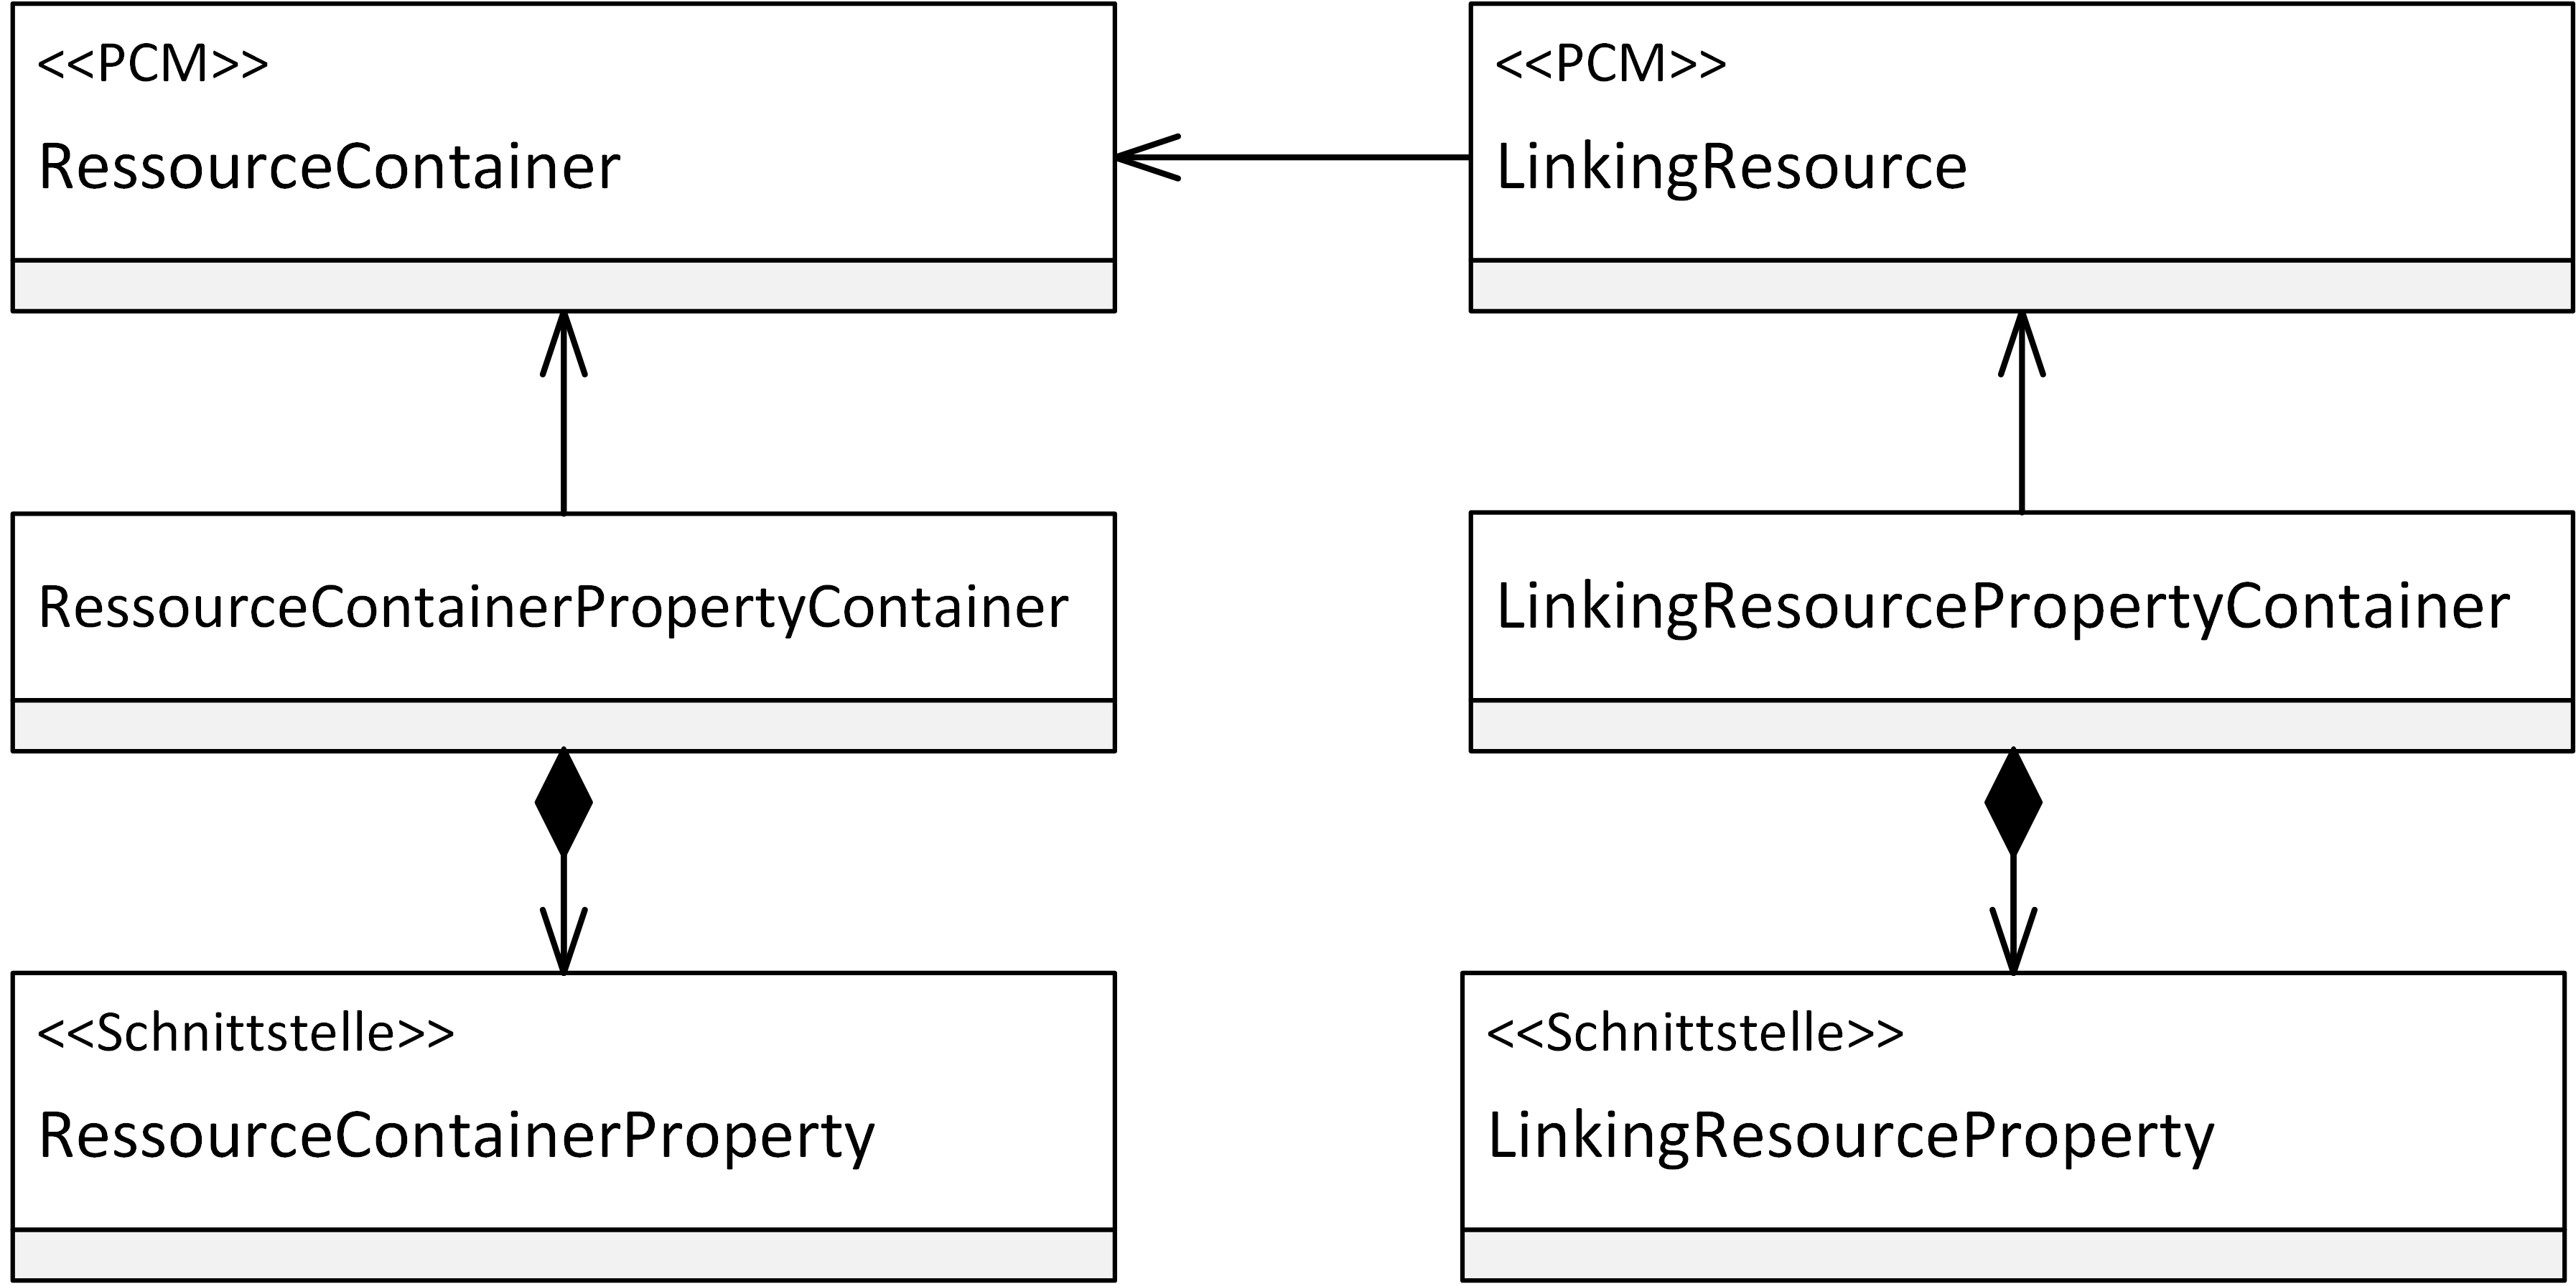
\includegraphics[width=0.75\textwidth]{images/meta_stereotypes_ubersicht.png}
	\caption{Übersicht der Erweiterung für das Ressourcen-Umgebungs-Modell}
	\label{img:modell:stereotypes:übersicht}
\end{figure}
Die Eigenschaften, die einen Resource-Container erweitern können sind in Abbildung \ref{img:modell:stereotypes:properties} abgebildet. Zu diesen Eigenschaften gehört die \texttt{Runtime}-Eigenschaft. Diese Eigenschaft sagt aus, ob auf dem Resource-Container noch weitere Software genutzt wird oder ob alles modelliert wurde. Um das zu spezifizieren, gibt es zwei Optionen. Diese werden in der Aufzählung \texttt{Runtime} modelliert. Wenn weitere Software auf dem Resource-Container genutzt wird, kann das mit \textit{shared} modelliert werden. Wenn aber keine weitere Software auf dem Resource-Container genutzt wird, kann dies mit \textit{exclusive} modelliert werden. Möchte man angeben wo sich ein Resource-Container befindet, erweitert man diesen mit der \texttt{Location}-Eigenschaft. Möchte man den Resource-Container mit einem Sicherheitsmechanismus schützen, erweitert man diesen mit der Eigenschaft \texttt{TamperProtection}. Dadurch lässt sich ein Sicherheitsmechanismus spezifizieren, der den Resource-Container vor Angriffen schützen soll. \par
\begin{figure}[h]
	\centering
  	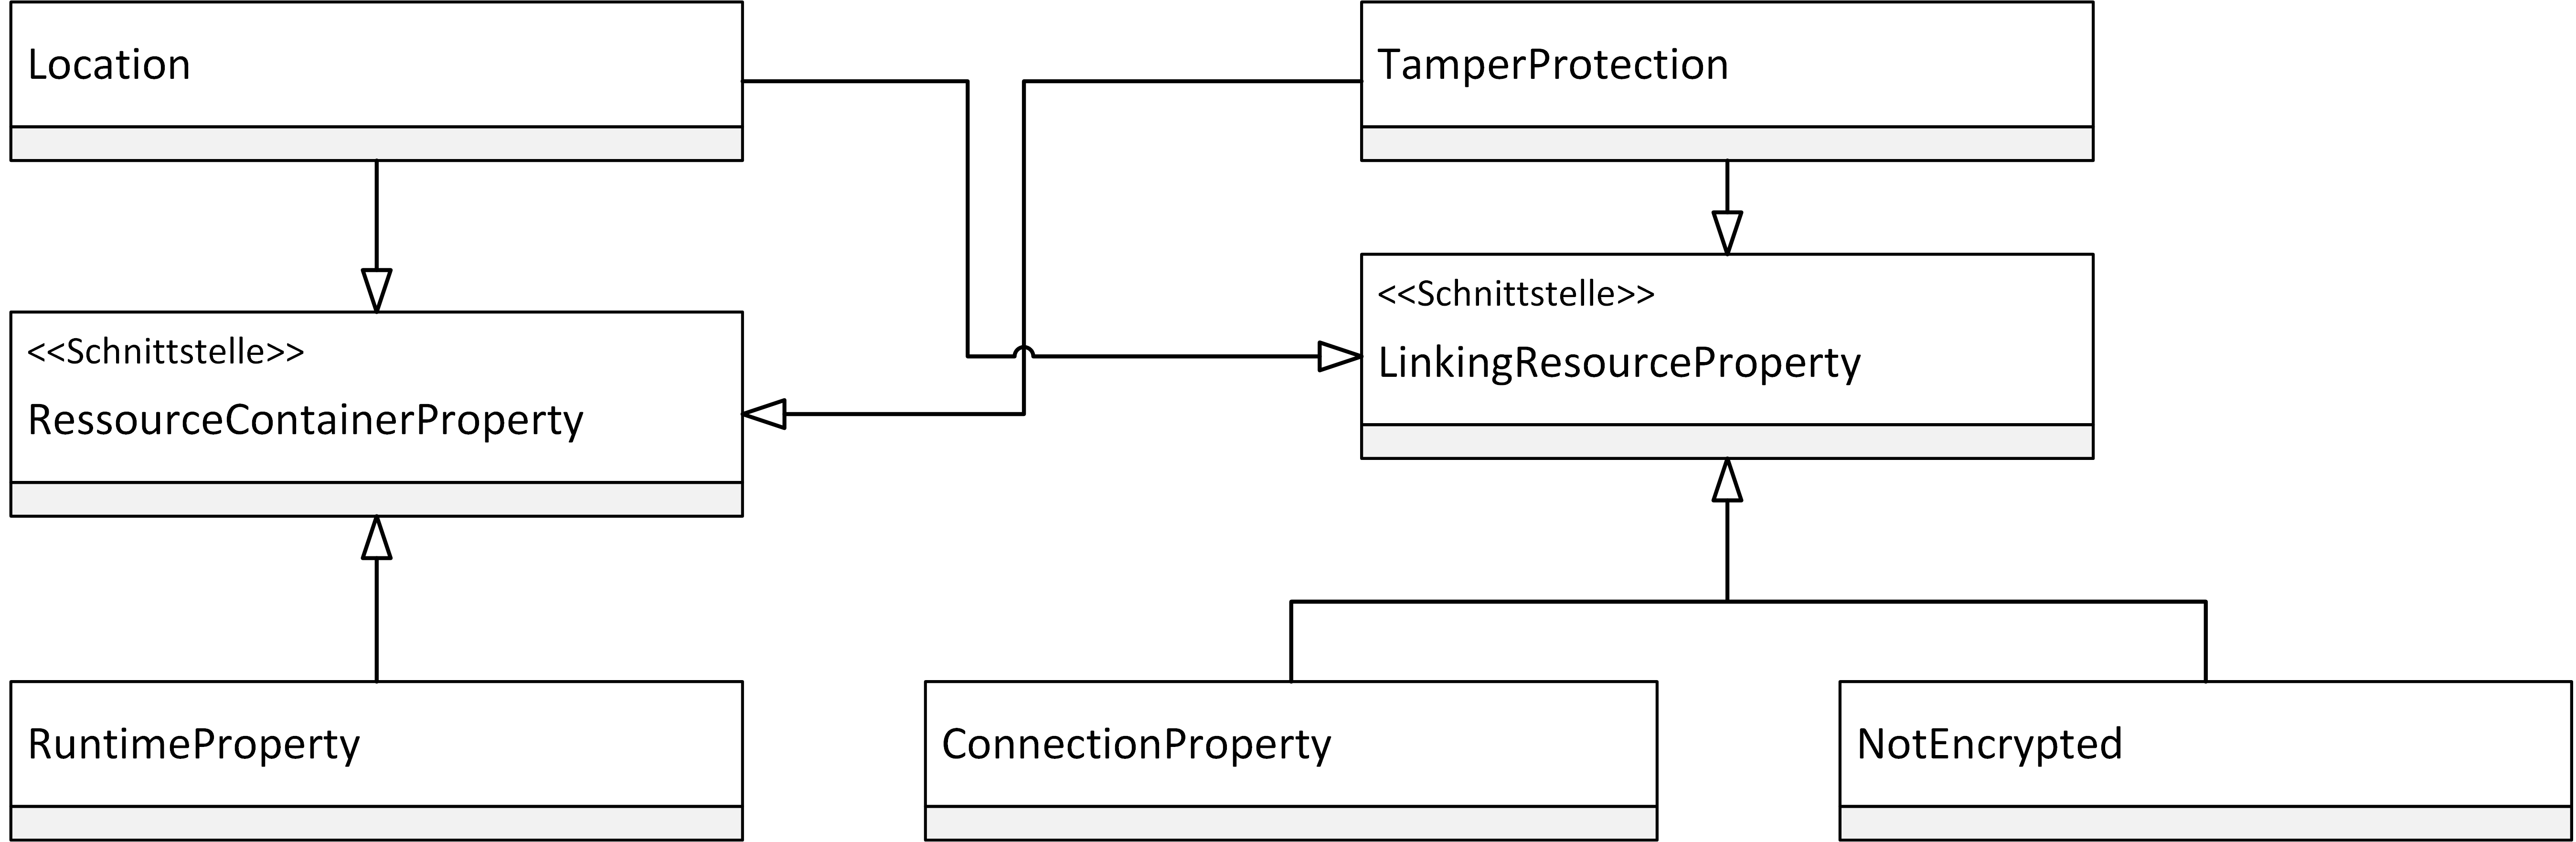
\includegraphics[width=1\textwidth]{images/meta_stereotypes_properties.png}
	\caption{Übersicht der Eigenschaften für Resource"=Container und Linking"=Resource}
	\label{img:modell:stereotypes:properties}
\end{figure}
In \autoref{img:szenario:rc} ist eine mögliche Modellierung eines Resource-Containers des Beispiels aus \autoref{sec:szenario} dargestellt. 
Dabei ist das Kreditkartenlesegerät (\textit{CCReader}) als Resource-Container modelliert. Auf den Resource-Container verweist ein \\\texttt{ResourceContainerPropertyContainer}. Dieser sammelt alle Eigenschaften, die an das Kreditkartenlesegerät angehängt werden sollen. Dazu gehört die \texttt{Runtime}-Eigenschaft. Sie ist hier \textit{exclusive}, da keine weitere Software auf dem Kreditkartenlesegerät genutzt wird. Eine weitere Eigenschaft, die angehängt wird, ist  \texttt{TamperProtection}. Das Kreditkartenlesegerät wird mit einem Passwort vor unbefugten Zugang geschützt. Schließlich wird mit der \texttt{Location}-Eigenschaft festgelegt, dass das Kreditkartenlesegerät sich im zweiten Raum des Ladens befindet. 

\begin{figure}[h]
	\centering
  	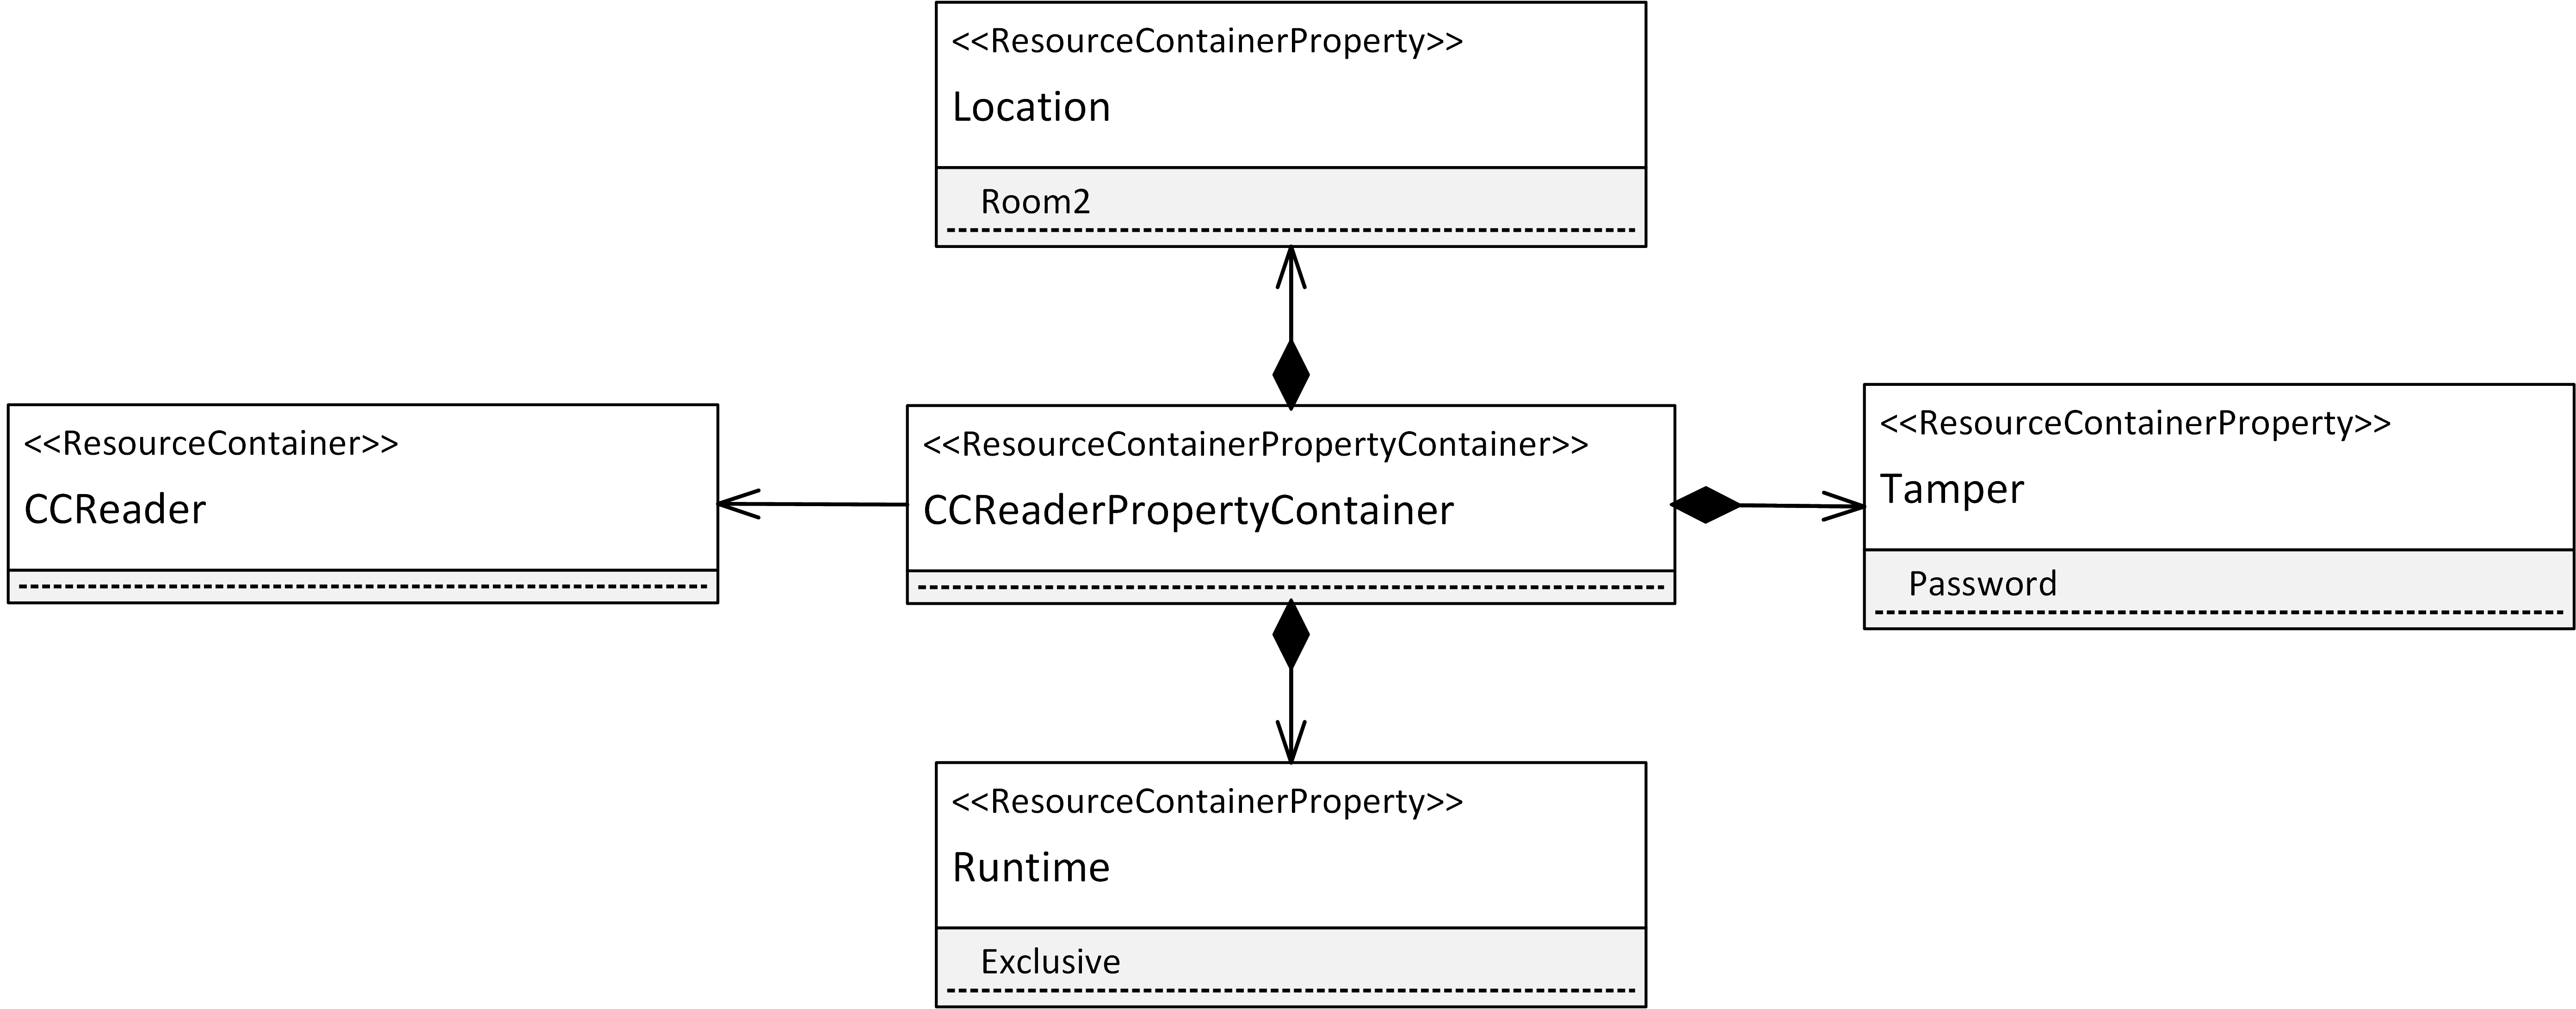
\includegraphics[width=1\textwidth]{images/szenario_rc.png}
	\caption{Resource-Container Beispiel des Laden-Szenarios}
	\label{img:szenario:rc}
\end{figure}

Auch die Linking-Resource kann mit Eigenschaften erweitert werden. Diese sind auch in \autoref{img:modell:stereotypes:properties} abgebildet. Eine Eigenschaft, die Linking-Resource erweitern kann, ist \texttt{Connection}. Diese Eigenschaft gibt an, ob es weitere Verbindungen auf der Linking"=Resource gibt, die aber nicht modelliert wurden. Die Optionen die dabei angegeben werden können sind in der Aufzählung \texttt{Connection} modelliert. Mit \textit{complete} wird signalisiert, dass es keine weiteren Verbindungen gibt. Wenn es weitere Verbindungen gibt, die nicht modelliert wurden, kann dies mit \textit{existing} modelliert werden. Schließlich kann ein Resource-Container Ports enthalten, die nicht verwendet werden, aber eine Verbindung an diesem möglich wäre. Dies kann mit \textit{possible} modelliert werden. Die Eigenschaft \texttt{NotEncrypted} gibt an, ob etwas auf der Linking-Resource nicht verschlüsselt wird, z.B. Protokolle oder Datengröße. Die beiden Eigenschaften \texttt{Location} und \texttt{TamperProtection} sind analog zum Resource-Container. \par
In \autoref{img:szenario:lr} ist eine mögliche Modellierung einer Linking-Resource des Beispiels aus \autoref{sec:szenario} abgebildet. Hier ist die Internetverbindung zwischen dem Kreditkartenlesegerät des Ladens und der Bank des Kundens als Linking-Resource modelliert. Auf die Linking-Resource verweist ein \texttt{LinkingResourcePropertyContainer}. Dieser sammelt alle Eigenschaften, die an die Linking-Resource angehängt werden sollen. Dazu gehört die \texttt{Location}-Eigenschaft. Sie spezifiziert als Ort, für die Linking-Resource, das Internet. Geschützt ist die Linking-Resource mit einem Passwort. Dies ist in der Eigenschaft \texttt{TamperProtection} spezifiziert. Außerdem wird spezifiziert, dass das Protokoll, über das kommuniziert wird, nicht verschlüsselt wird. Mithilfe der Eigenschaft \texttt{NotEncrypted} wird dies modelliert. Schließlich wird mit der \texttt{Connection}-Eigenschaft angegeben, dass es keine weiteren Verbindungen, außer den modellierten gibt (\textit{complete}). 

\begin{figure}[h]
	\centering
  	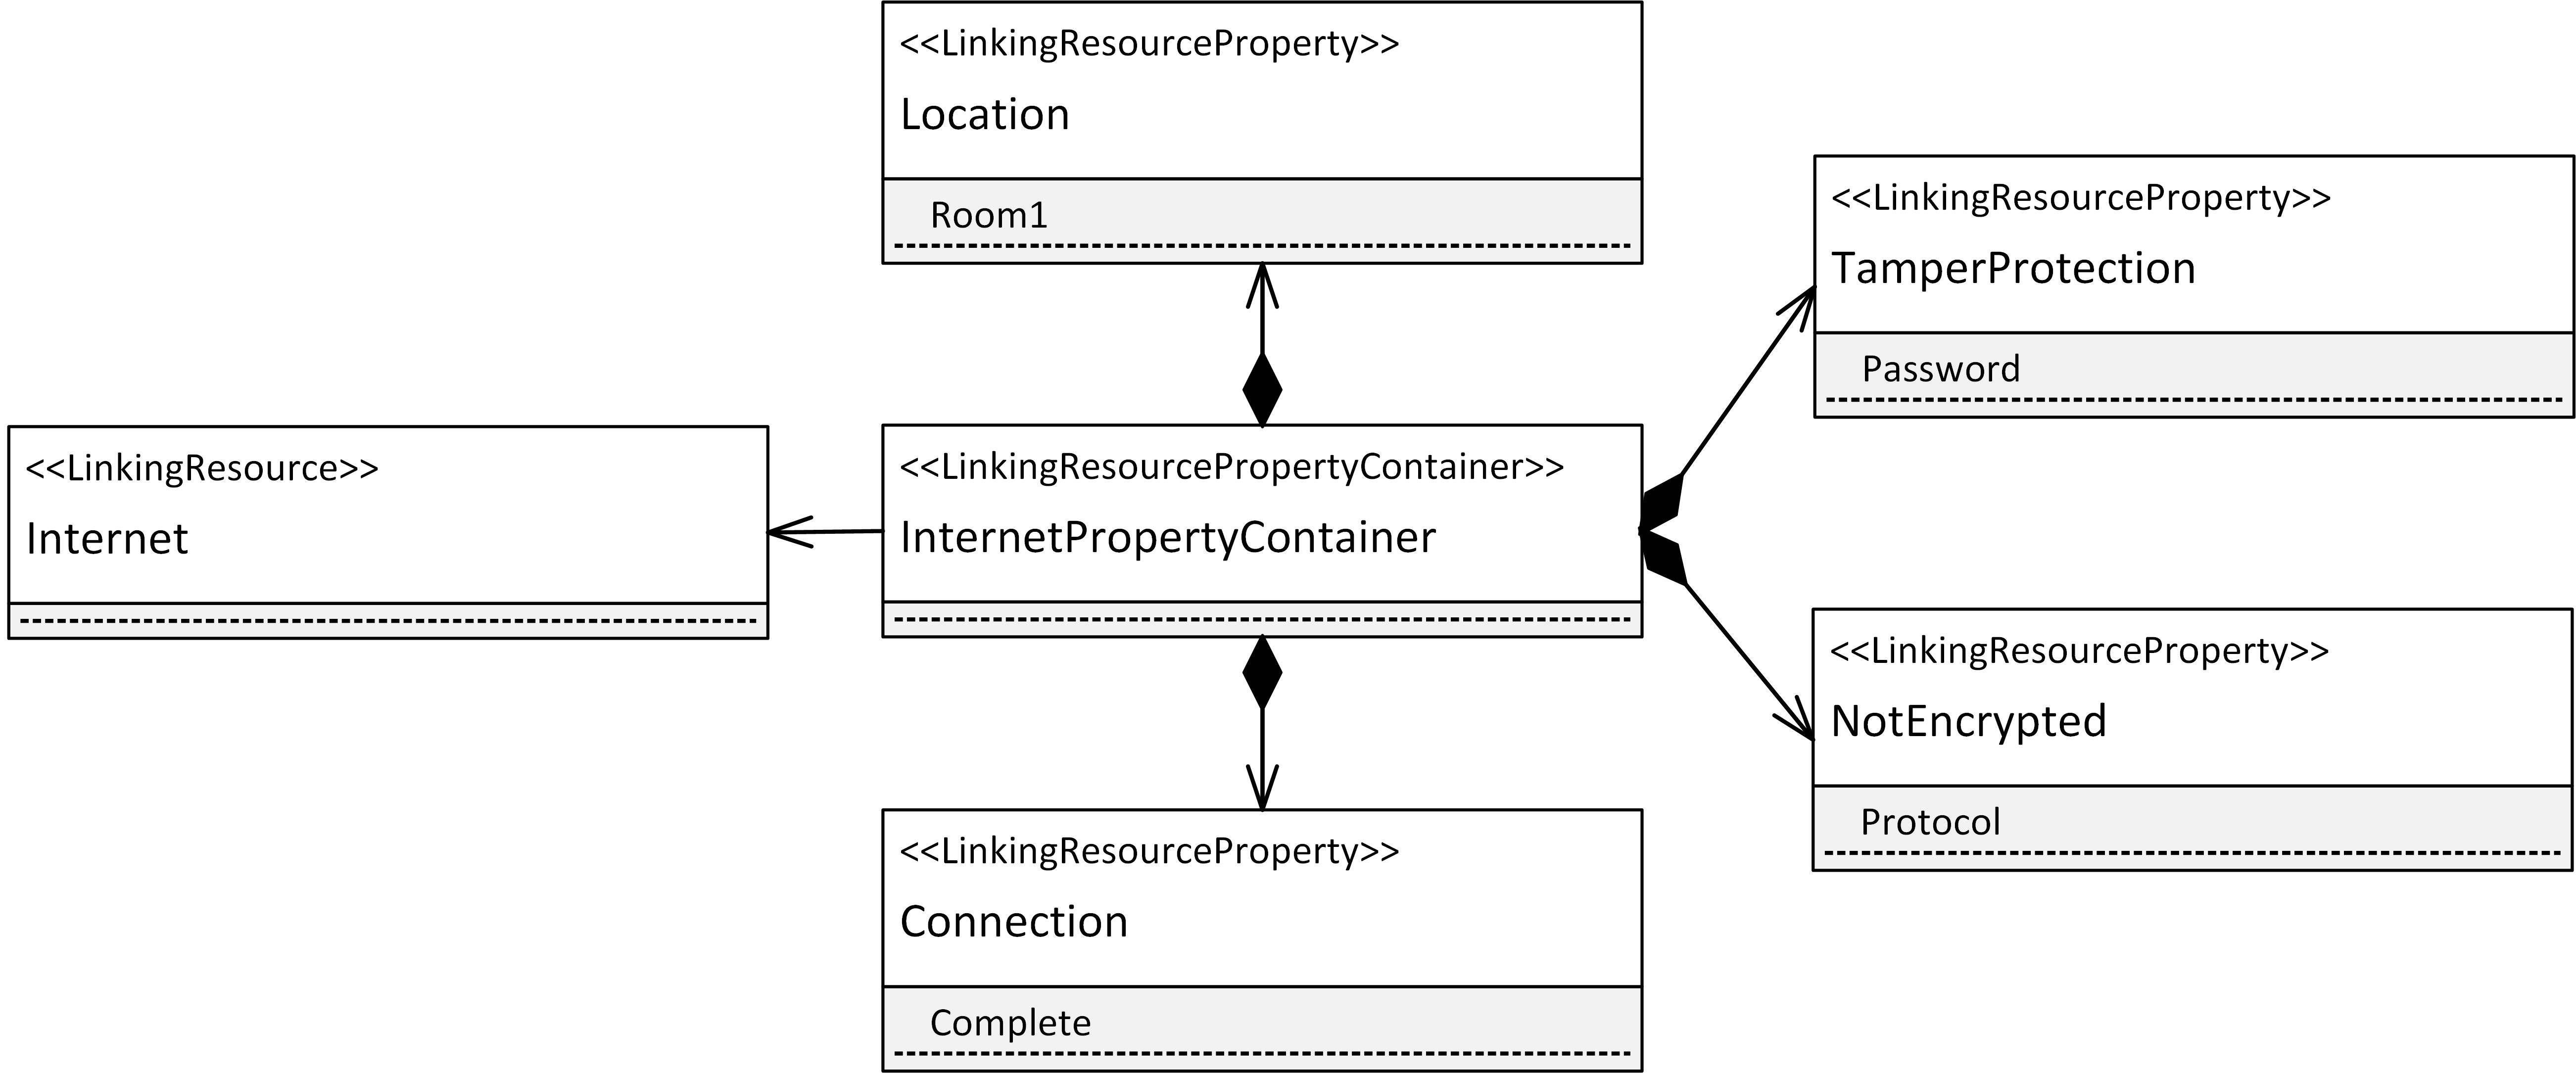
\includegraphics[width=1\textwidth]{images/szenario_lr.png}
	\caption{Linking-Resource Beispiel des Laden-Szenarios}
	\label{img:szenario:lr}
\end{figure}

\section{Datenmodellierer}
\label{sec:data}
In diesem Abschnitt, wird die Modellierung von Daten beschrieben, die in einem System verarbeitet werden. Dabei handelt es sich nicht um individuelle Daten, sondern um Datenklassen. Das können z.B. Daten sein, die für einen Kauf benötigt werden, wie Name oder Adresse. Das bedeutet, dass der Benutzer die Datenklasse \texttt{Namen} in den Dienst eingibt und nicht einen speziellen Namen. Die Daten werden vom Komponentenentwickler sowie dem Domänenexperten im Ressourcen-Umgebungs-Modell und Nutzungsmodel eingesetzt. In \autoref{img:modell:data} ist diese Modellierung abgebildet. \par
Die Klasse \texttt{Data} repräsentiert dabei eine Datenklasse. An \texttt{Data} können Eigenschaften (\texttt{DataProperty}) angehängt werden. Mithilfe eines \texttt{DataPropertyContainers} werden die Eigenschaften gesammelt und an eine Datenklasse gehängt. Die Eigenschaften können je nach untersuchtem Qualitätsattribut unterschiedlich sein. Sie können daher variabel gewählt werden. Für Datenflussanalysen können so Sicherheitseigenschaften spezifiziert werden. Darauf aufbauend ist eine Überprüfung der Einhaltung dieser Eigenschaften möglich. Außerdem befindet sich in dem Paket das Element \texttt{DataSet}. Ein \texttt{DataSet} ist eine Gruppierungen von Datenklassen. Daten können so verschiedene Gruppierungen zugeordnet werden. Im Anschluss kann, in Hinblick auf eine Datenflussanalyse, festgelegt werden, welche Person Zugriff auf welche \texttt{DataSet}s haben soll. Während der Datenflussanalyse kann schließlich geprüft werden, ob jeder nur Zugriff auf die \texttt{DataSet}s hat, auf die er zugreifen darf. \par
\begin{figure}[h]
	\centering
  	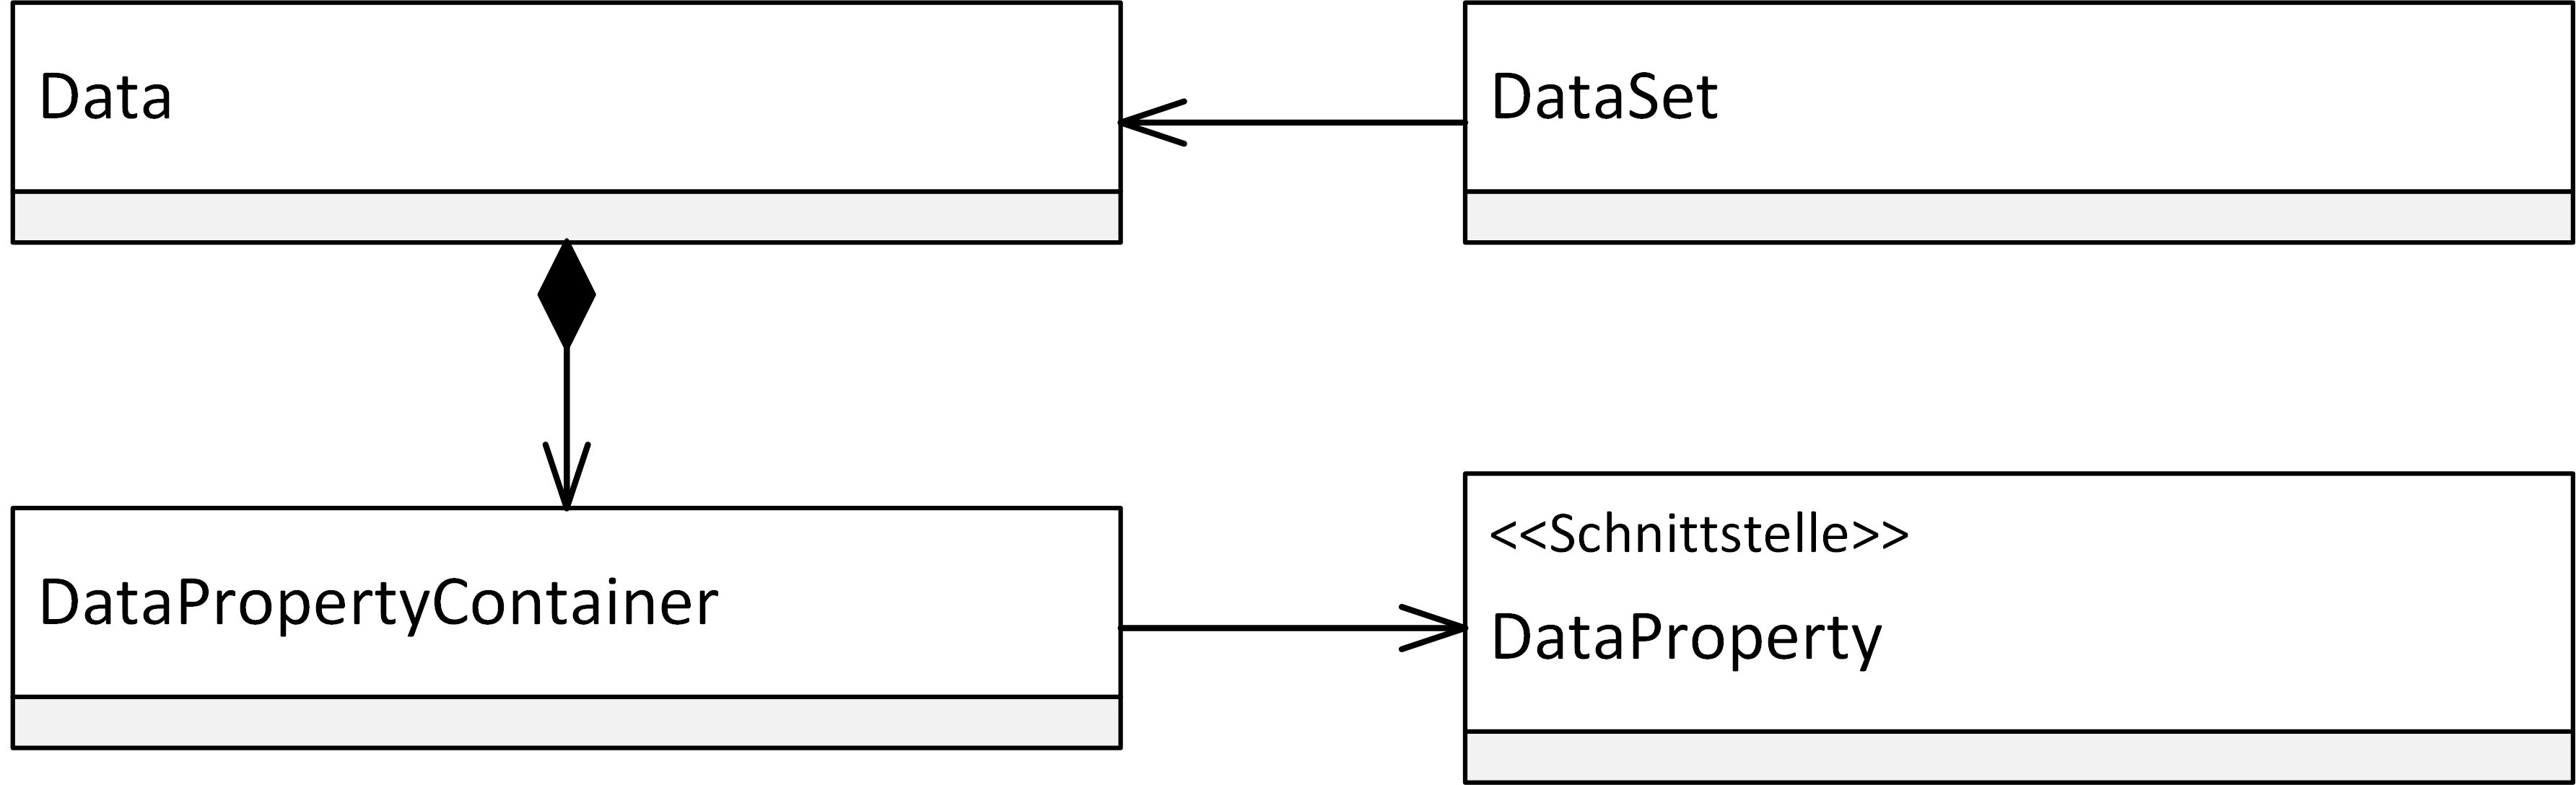
\includegraphics[width=0.8\textwidth]{images/meta_data.png}
	\caption{Übersicht der Datenmodellierung}
	\label{img:modell:data}
\end{figure}
In dem Beispielszenario aus \autoref{sec:szenario} wären \textit{Kreditkartendaten}  eine Datenklasse und \textit{Kunde}, \textit{Besitzer} und \textit{Warenlager} als \texttt{DataSet} modelliert. Dabei sind die \textit{Kreditkartendaten} nur im \texttt{DataSet} \textit{Kunde}. Das heißt, dass nur Personen, die dem \texttt{DataSet} \textit{Kunde} zugewiesen sind, Zugriff auf die Daten haben. Bei einer Datenflussanalyse kann nun geprüft werden, ob die \textit{Kreditkartendaten} bei einer Person oder einem System ankommen, die eigentlich keinen Zugriff auf diese haben sollte. 

\section{Komponentenentwickler}
\label{sec:paket:dfseff}
In diesem Abschnitt wird die Modellierung für einen \gls{dfseff} beschrieben. Mit diesem \gls{dfseff} kann der Komponentenentwickler einen Datenfluss innerhalb einer Komponente, in Form eines \gls{seff}, modellieren. Dabei soll es möglich sein Daten zu verfeinern, indem man diese mit Parametern verknüpft. Außerdem soll der Datenfluss über mehrere Datenverarbeitungsschritte modelliert werden können und schließlich ein globaler Datenfluss aus dem Nutzungs-, Komponenten-Repository-, Ressourcen-Umgebungs-, Komponenten-Allokations- und System-Modell abgeleitet werden. Vor der Meta-Modell-Bildung muss überlegt werden, ob Elemente aus dem \gls{pcm} wiederverwendet werden können. Das war in den Abschnitten davor nicht nötig, da es nichts Vergleichbares in Palladio gab. In Palladio existiert aber bereits ein \gls{seff}. Der \gls{rdseff}, der eine \gls{seff}-Spezialisierung für Performanzvorhersagen darstellt. \par 
Als ein Elemente, das wiederverwendet werden kann, wurde die \texttt{Signatur} identifiziert. Eine \texttt{Signatur} modelliert die Signatur einer Methode. Dazu zählen Parameter, der Rückgabetyp und Fehlerspezifikationen. Der Vorteil dieser Wiederverwendung ist, dass der Komponentenentwickler seine bereits modellierten Signaturen wiederverwenden kann. Außerdem geht der Zusammenhang zwischen Kontroll- und Datenfluss nicht verloren. Ein weiteres Element, das wiederverwendet werden kann, ist \texttt{Parameter}. \texttt{Parameter} modelliert einen Parameter einer \texttt{Signatur}. \texttt{Parameter} besteht aus einem Namen und einem Datentyp.  
Die Vorteile sind ähnlich zu denen der \texttt{Signatur}. \texttt{Parameter} ist nicht vom \gls{rdseff} abhängig. Außerdem geht der Zusammenhang zwischen Kontroll- und Datenfluss nicht verloren. Alternativ wäre hier ein neues Parameter Element möglich, dass direkt Daten und Parameter verknüpft. Jedoch hat bei dieser Modellierung der Benutzer wenig Mehrwert und muss stattdessen evtl. bereits modellierte Parameter neu modellieren. \par
Elemente, die hingegen nicht wiederverwendet werden können, sind \texttt{AbstractAction}, ihre Unterklassen und \texttt{ResourceDemandingBehaviour}. \texttt{AbstractAction} modelliert dabei einen Aufruf zu einem internen oder externen Dienst. Außerdem hat \texttt{AbstractAction} eine Referenz zu \texttt{ResourceDemandingBehaviour}. Dieses Element modelliert das Verhalten einer Komponente als Sequenz von \texttt{AbstractAction}s. Durch die Wiederverwendung der Elemente würden auch eine Vielzahl anderer Elemente im \gls{dfseff} verwendbar werden, die aber an dieser Stelle keinen Sinn machen. Ein Beispiel wäre hier die \texttt{ReleaseAction}, die eine Unterklasse von \texttt{AbstractAction} ist. Die \texttt{ReleaseAction} gibt Ressourcen im \gls{rdseff} wieder frei. Da Ressourcen für die untersuchte Analyse nicht benötigt werden, ist eine Wiederverwendung an dieser Stelle nicht sinnvoll. \par
Eine Übersicht des Meta-Modells ist in \autoref{img:modell:dfseff:übersicht} abgebildet. Das Root-Element, dieser Erweiterung, ist das Element \texttt{DataFlowSEFF}. Aufgrund einer Containment"=Beziehung zwischen den Elementen \texttt{BasicComponent} und \texttt{ServiceEffectSpecification} kann das Element \texttt{ServiceEffectSpecification} nicht wiederverwendet werden. \\\texttt{ServiceEffectSpecification} ist eine abstrakte Klasse und modelliert dabei einen \gls{seff}. Spezielle \gls{seff}s sollten von dieser Klasse erben. Stattdessen referenziert das Element \\\texttt{DataFlowSEFF} die Elemente \texttt{BasicComp-\\onent} und \texttt{Signature}. Eine \texttt{BasicComponent} modelliert in \gls{pcm} eine Komponente. Komponenten können dabei abstrakt oder konkret sein. Abstrakte Komponenten spezifizieren nur ihre Schnittstellen und werden vom Software-Architekten als Platzhalter verwendet. Sie werden im weiteren Verlauf der Bachelorarbeit nicht näher betrachtet. Konkrete Komponenten sind entweder Basis Komponenten (\texttt{BasicComponent}) oder setzen sich aus mehreren zusammen. Eine \texttt{BasicComponent} spezifiziert dabei, für jede Operation die sie bereitstellt, ein Verhalten. Die zusammengesetzten Komponenten werden im Weiteren nicht näher betrachtet. \par 
Außerdem enthält \texttt{DataFlowSEFF} das Element \texttt{DataFlowBehavior}. \texttt{DataFlowBehavior} modelliert das Verhalten einer Komponente als Sequenz, die aus mehreren \texttt{DataFlow-\\AbstractActions} besteht.
\begin{figure}[h]
	\centering
  	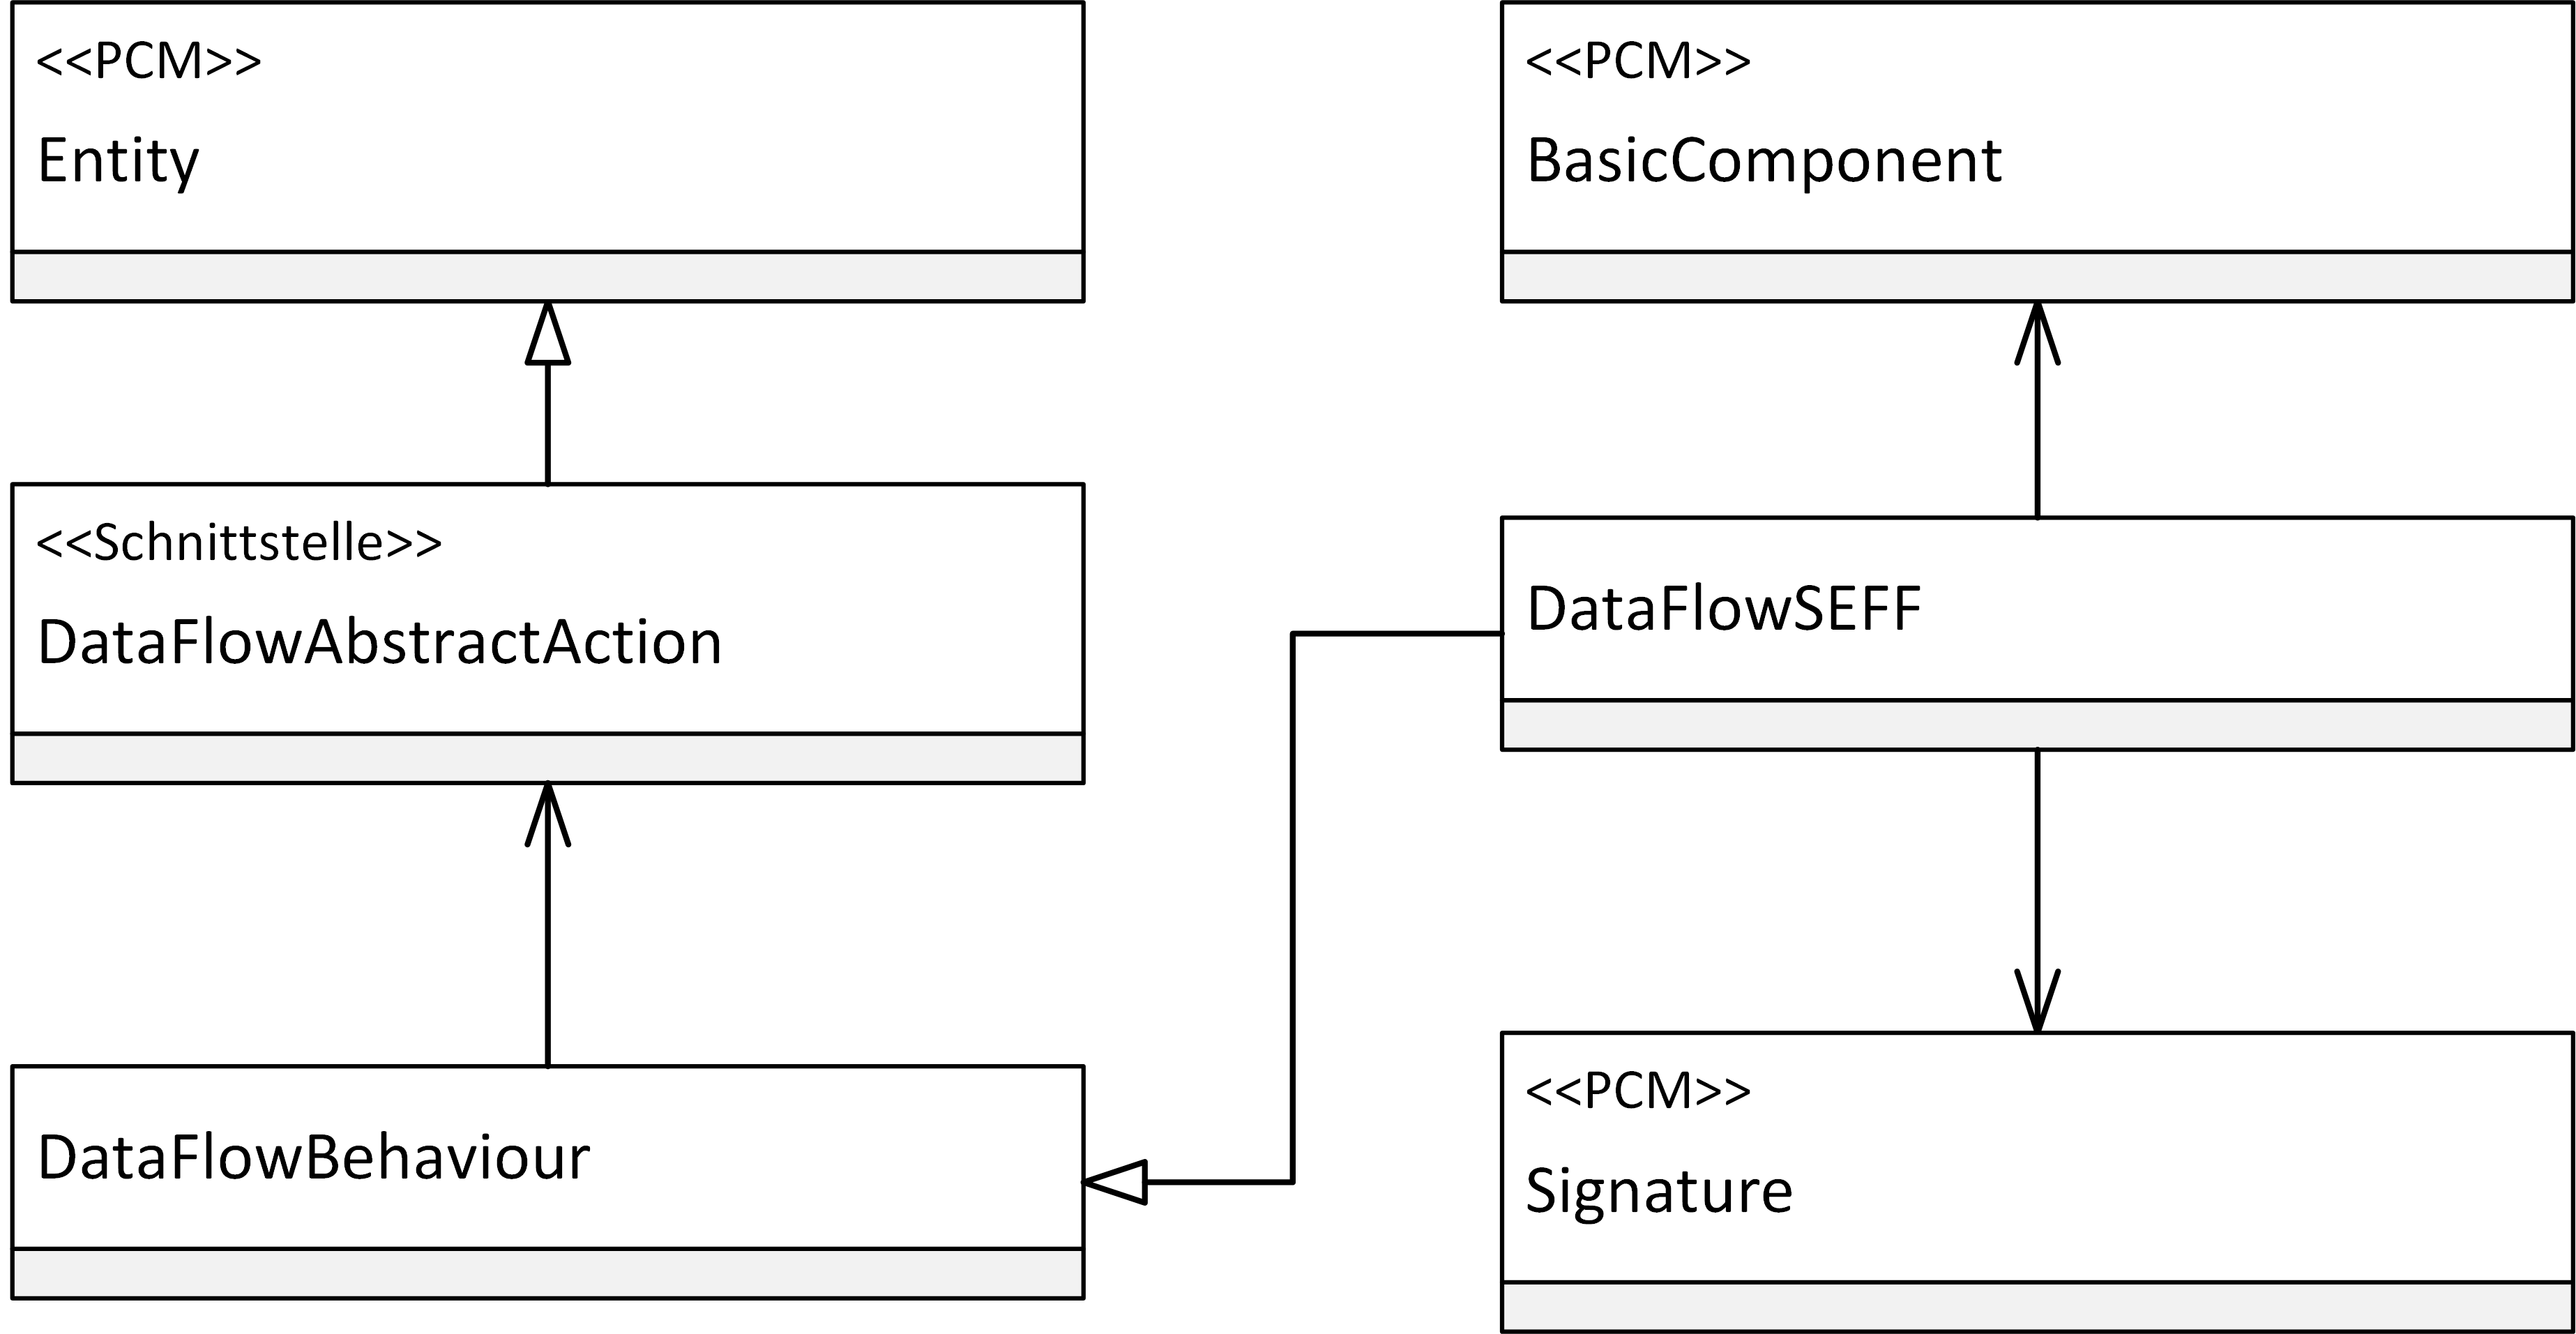
\includegraphics[width=0.8\textwidth]{images/meta_dfseff_ubersicht.png}
	\caption{Übersicht der DFSEFF Erweiterung}
	\label{img:modell:dfseff:übersicht}
\end{figure}
Der Ablauf eines \gls{dfseff} ist ähnlich eines UML"=Aktivitätsdiagramm und des kontrollflussorientierten \gls{seff}s. Die verschiedenen Elemente mit denen der Datenfluss beschrieben wird, sind in \autoref{img:modell:dfseff:actions} abgebildet. Ein \gls{dfseff} besteht aus einer \texttt{StartAction} und einer \texttt{StopAction}, die den Anfang und das Ende des Datenflusses kennzeichnen. Zwischen diesen beiden Elementen können ein Reihe anderer \texttt{DataFlowAbstractActions} eingegliedert werden. Dazu gehört die \texttt{DataFlowExternal-\\Action} und die \texttt{InternalDataSourceAction}. Beide Elemente sind, wie ihre Oberklasse, abstrakt und erlauben es um weitere Aktionen erweitert zu werden. Die \texttt{DataFlowExternal-\\Action} modelliert einen Aufruf eines Dienstes, der in einer Schnittstelle spezifiziert wurde. Eine \texttt{InternalDataSourceAction} gibt an, woher Daten stammen. In der jetzigen Modellierung unterteilt sie sich in \texttt{DataJoin} und \texttt{CreateData}. Bei \texttt{DataJoin} werden mehrere Daten zu einem neuen Datum vereinigt. \texttt{CreateData} hingegen erstellt ein neues Datum. Indem jeweils das Vorgänger und Nachfolger Feld der einzelnen \texttt{DataFlowAbstractAction}-Elemente spezifiziert wird, kann ein Datenfluss modelliert werden. \par
\begin{figure}[h]
	\centering
  	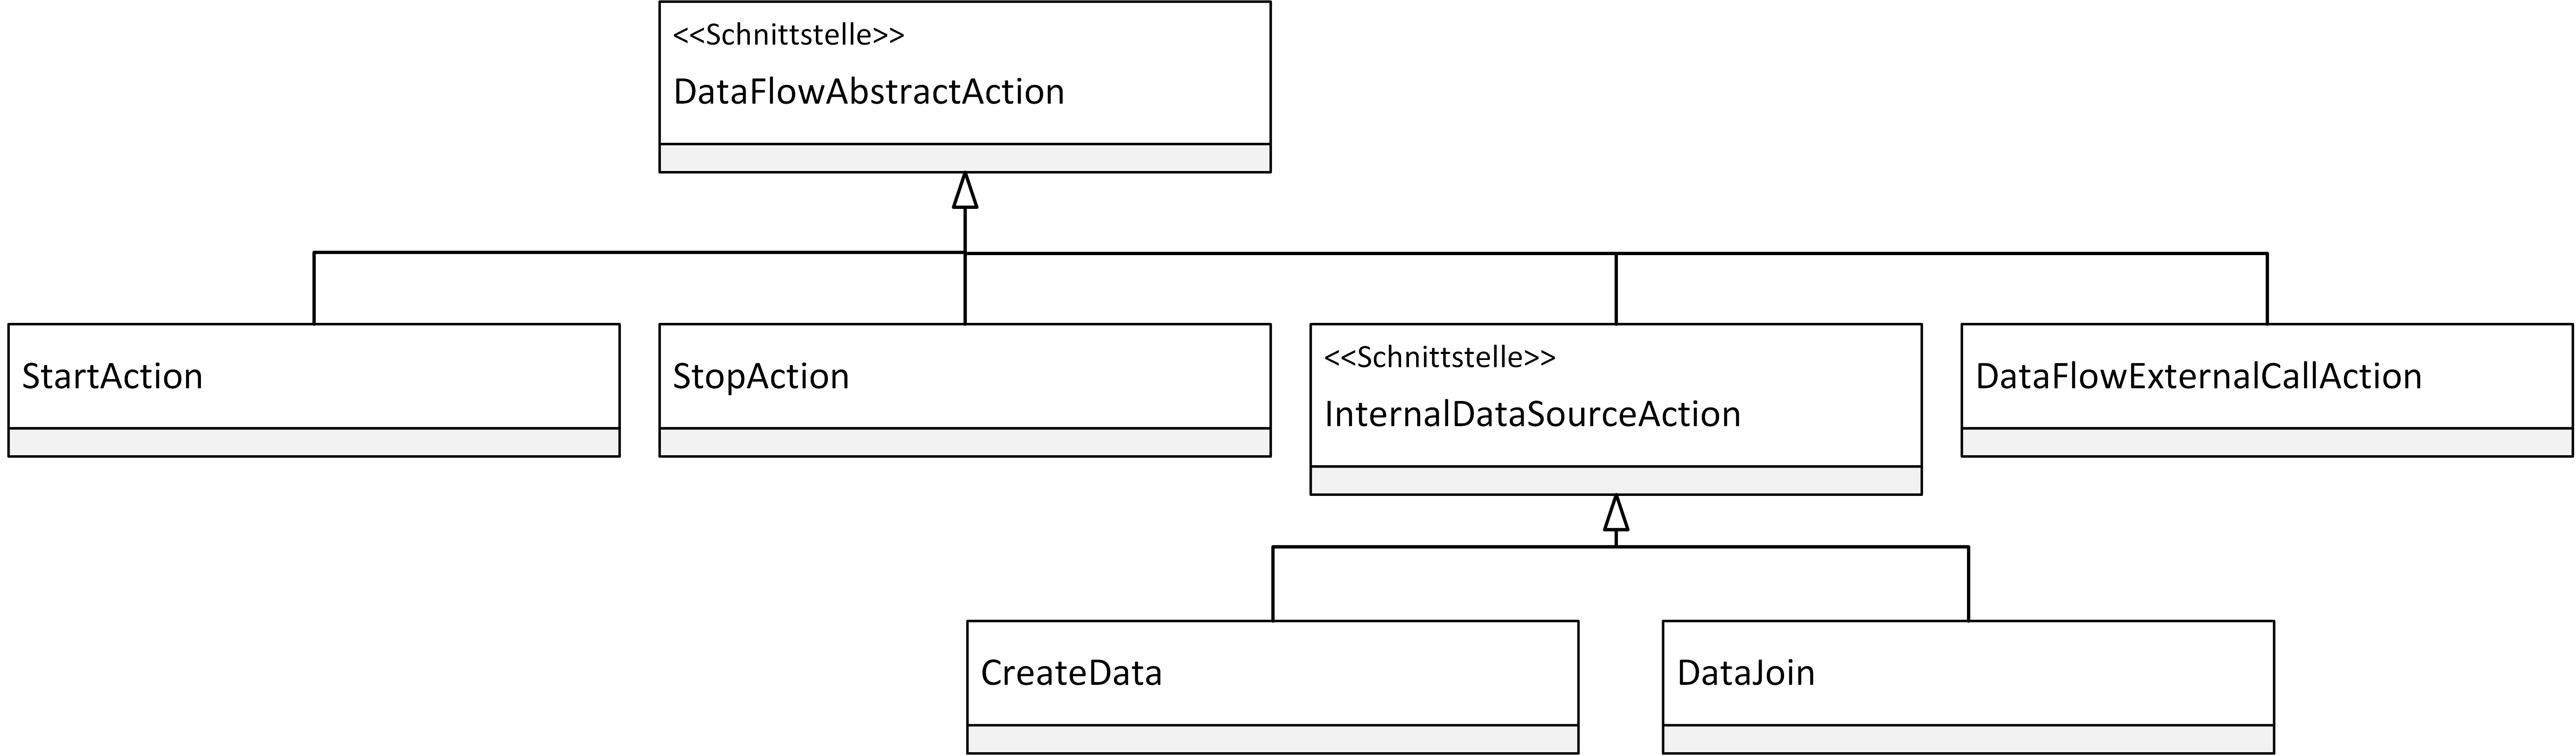
\includegraphics[width=1\textwidth]{images/meta_dfseff_actions.png}
	\caption{Übersicht der Aktionen des DFSEFF}
	\label{img:modell:dfseff:actions}
\end{figure}
Das wohl wichtigste Konzept des \gls{dfseff} ist die Möglichkeit Daten und Parameter zu verknüpfen. Dadurch können Daten durch das System verfolgt werden und schließlich in \texttt{DataSet}s eingeordnet werden. Die Modellierung dazu ist in \autoref{img:modell:dfseff:bindings} abgebildet. Mithilfe des Elements \texttt{VariableBinding} können \texttt{DataFlowExternalAction}s um eine Verknüpfung von Daten und Parameter erweitert werden. Diese Verknüpfung wird als \texttt{Binding} modelliert. Ein \texttt{Binding} besteht aus einem Parameter, der aus einer Signatur stammt, die die \texttt{DataFlowExternalAction} aufruft und einer Datenklasse. \texttt{Binding}s werden in \texttt{BindingContainer} gesammelt und gruppiert. \par
\begin{figure}[h]
	\centering
  	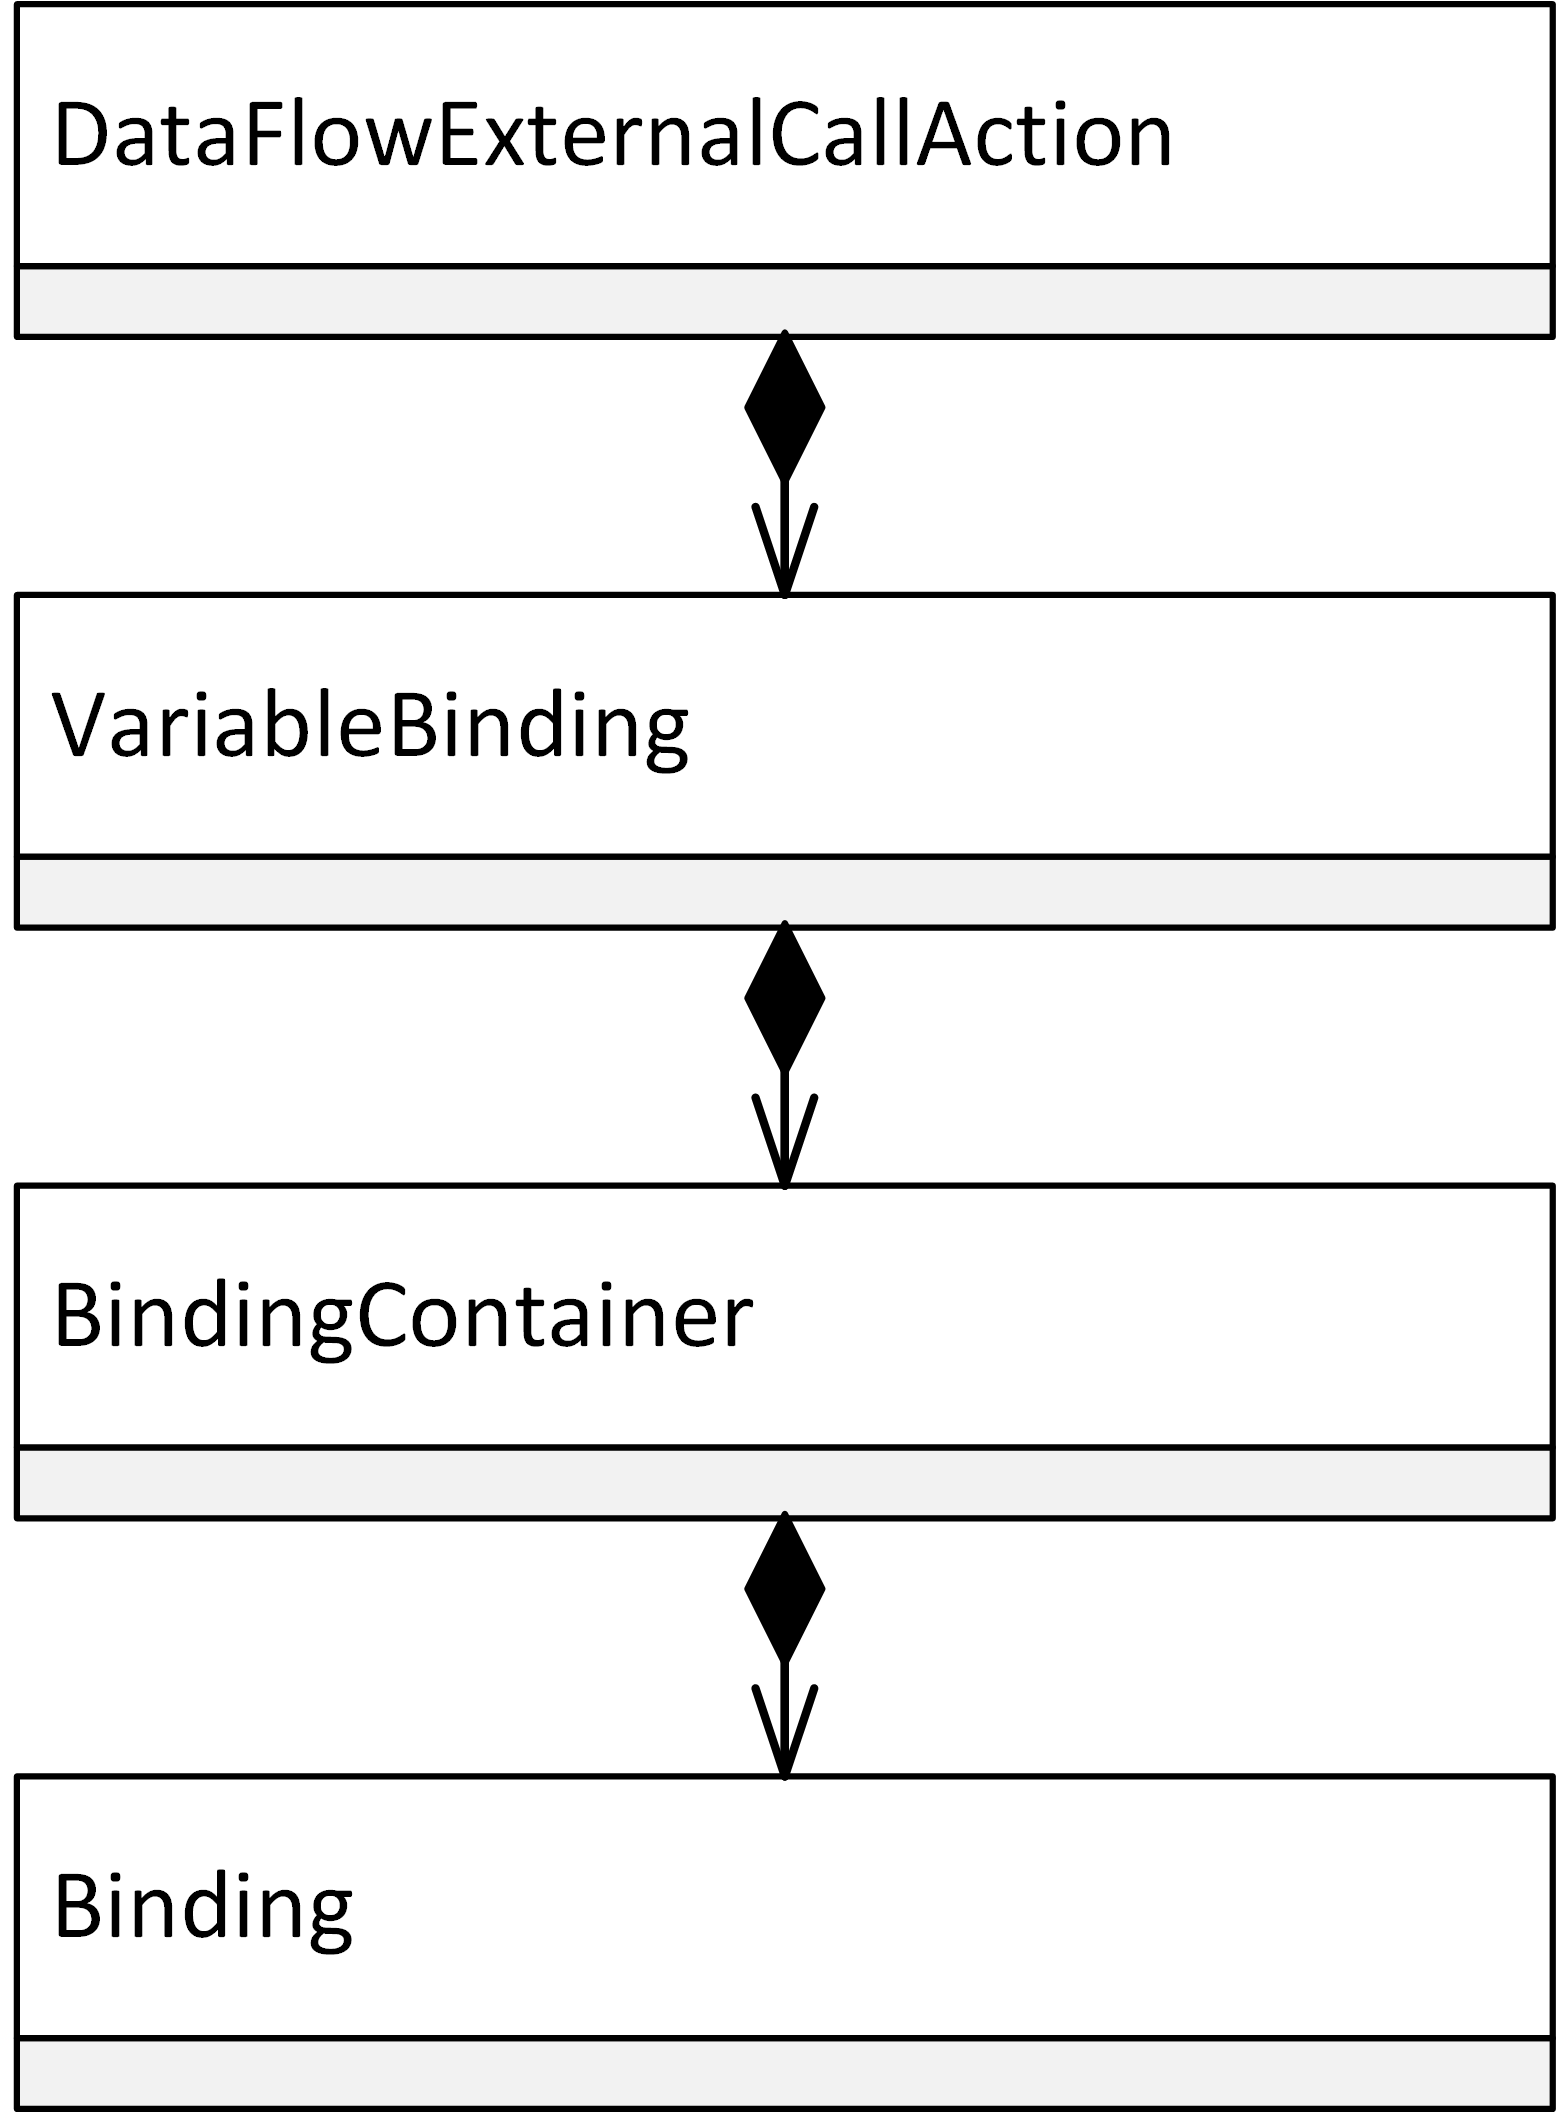
\includegraphics[width=0.35\textwidth]{images/meta_dfseff_bindings.png}
	\caption{Übersicht der Modellierung von \texttt{Binding}s}
	\label{img:modell:dfseff:bindings}
\end{figure}
In \autoref{img:szenario:seff} wurde der Datenfluss des Kaufvorgangs aus \autoref{sec:szenario} als \gls{dfseff} modelliert. In dieser Modellierung gibt es die Datenklasse \textit{ProductData}. Der Datenfluss fängt mit einer \texttt{DataFlowExternalAction} an, die den Dienst \texttt{checkForProduct(Product product)} aufruft. Sie enthält ein \texttt{Binding}, das den Parameter \textit{product} mit der Datenklasse \textit{ProductData} verknüpft. Als nächstes wird eine weitere \texttt{DataFlowExternalAction} ausgeführt. Sie ruft den Dienst \texttt{getProduct(Product product)} auf. Diese Aktion enthält ebenfalls ein \texttt{Binding}. Dieses verknüpft den Parameter \textit{product} mit der Datenklasse \textit{ProductData}. Schließlich wird mit \texttt{CreateData} ein neues Datum erstellt. Das neue Datum heißt \textit{Product}. Mit dieser letzten Aktion endet der Datenfluss.

\begin{figure}[h]
	\centering
  	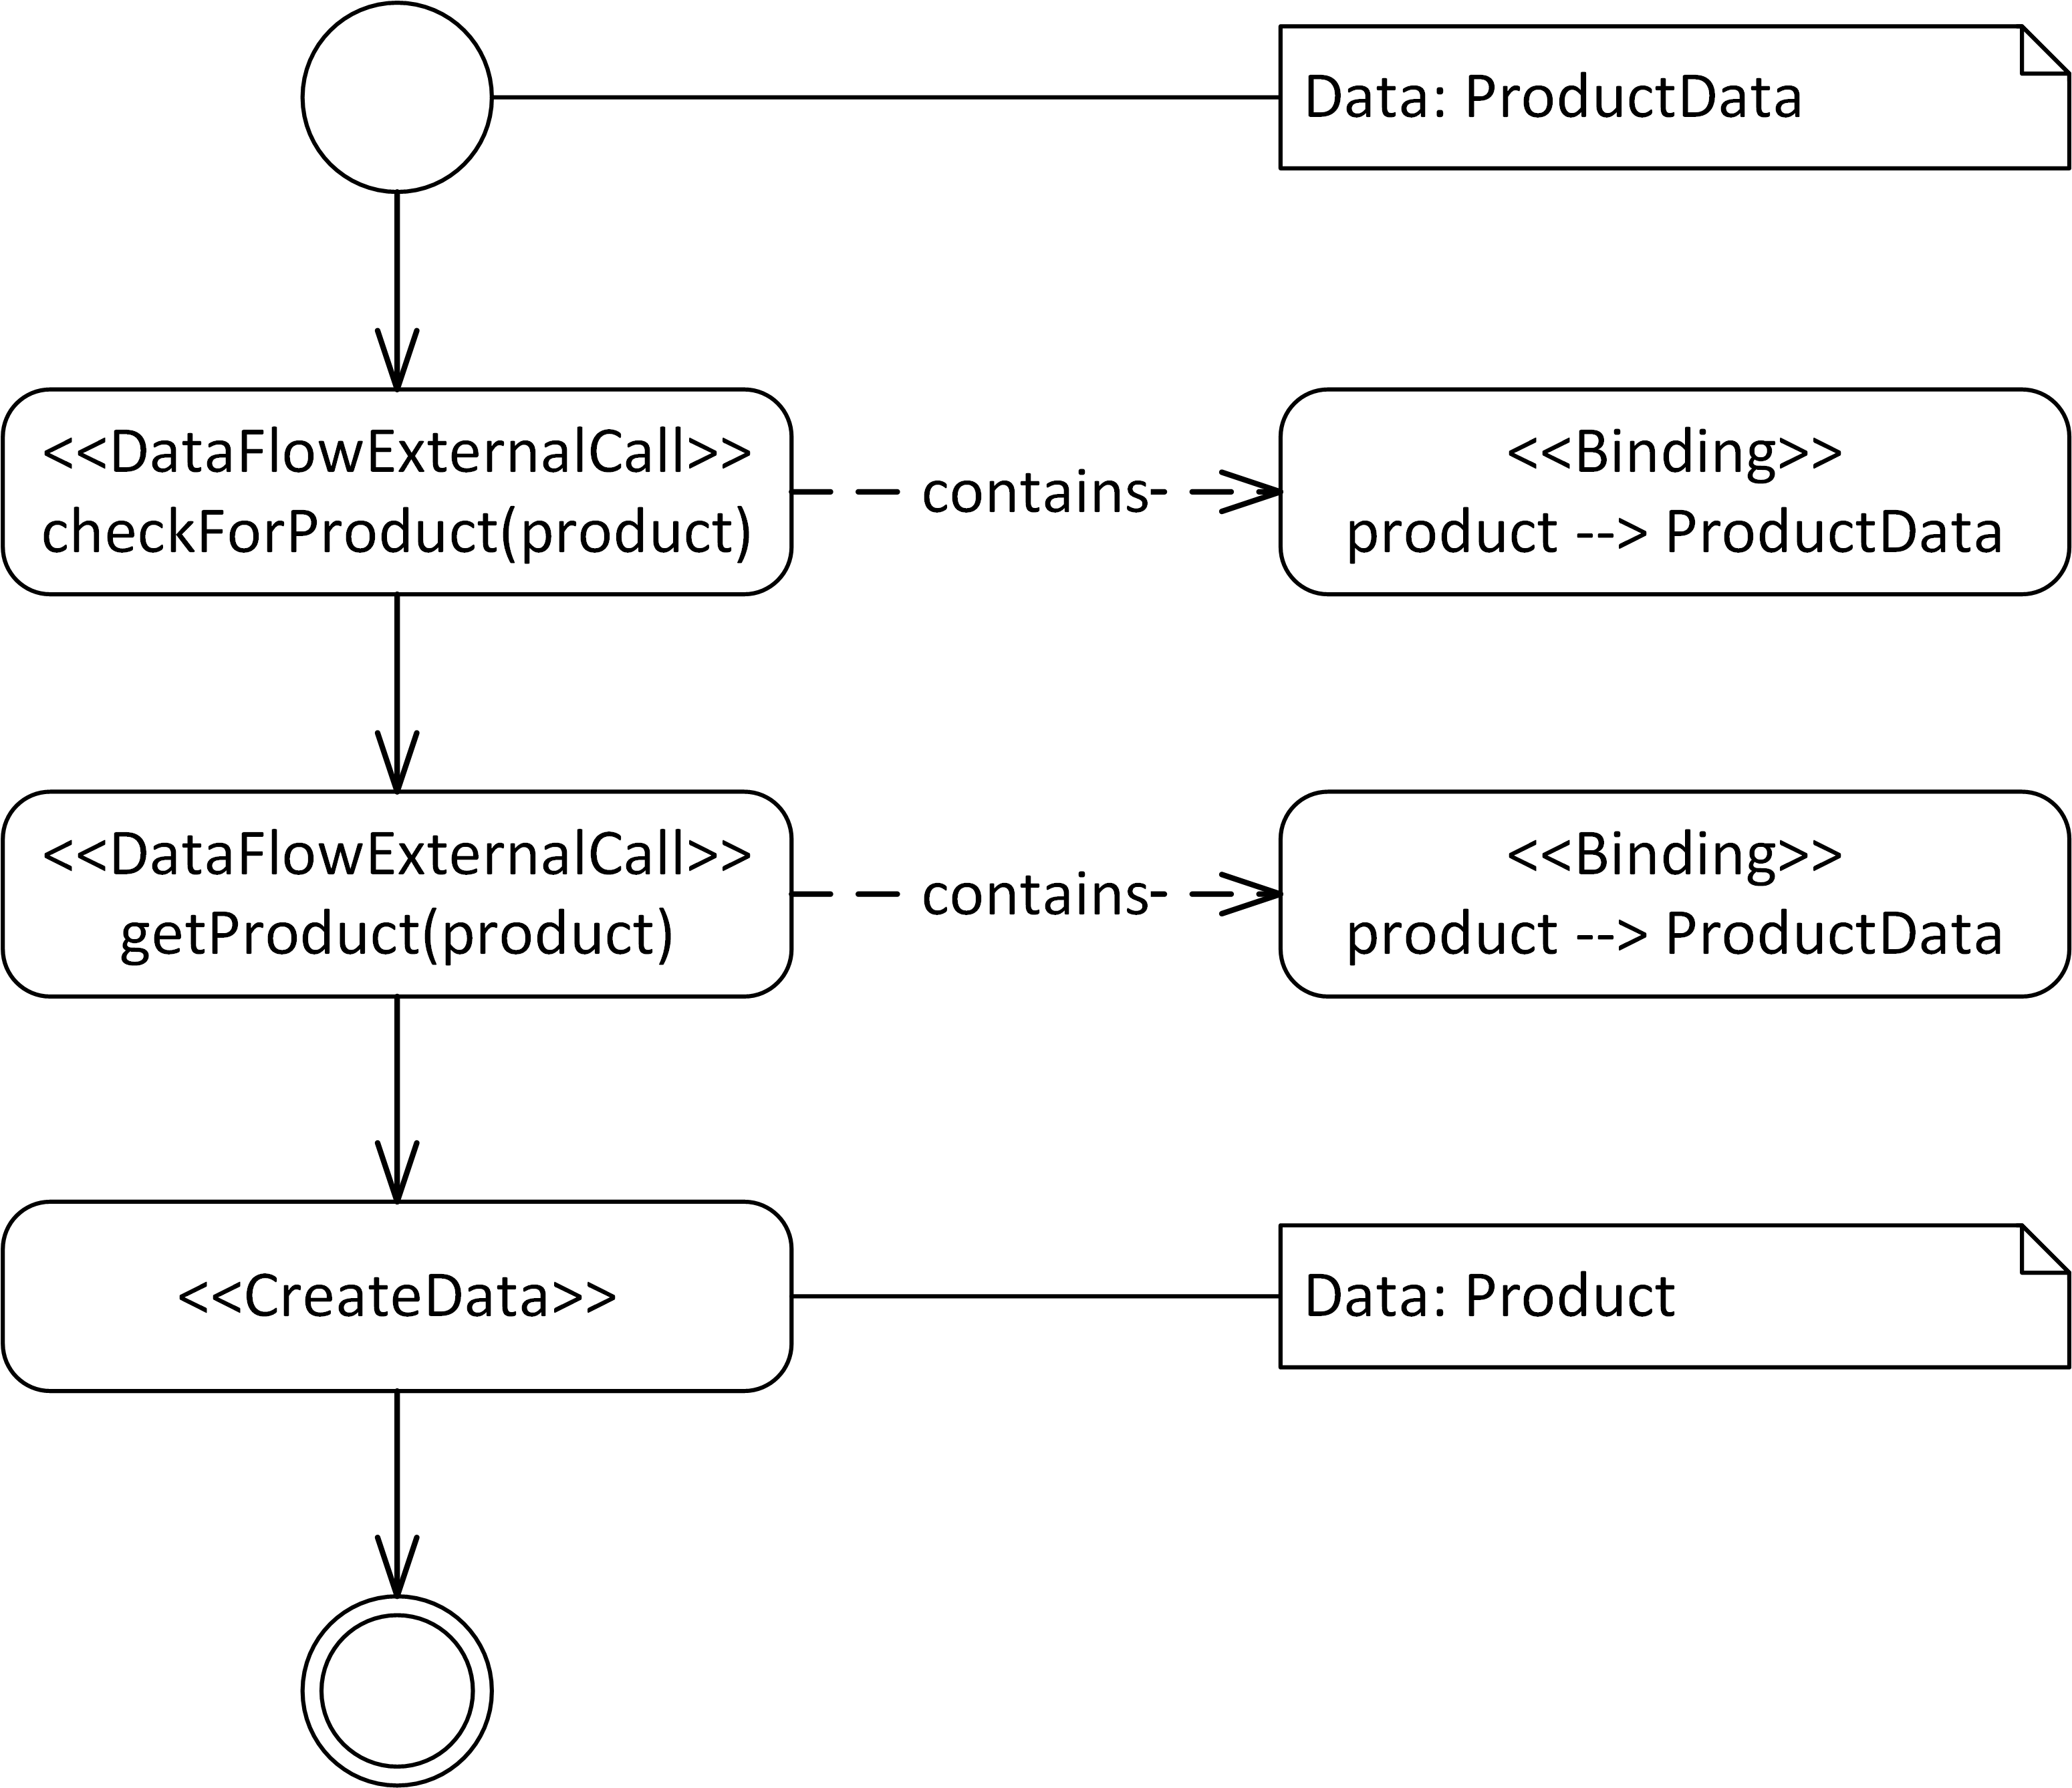
\includegraphics[width=0.7\textwidth]{images/szenario_seff.png}
	\caption{Datenfluss des Dienstes \texttt{buy(Product product)} aus dem Laden-Szenario}
	\label{img:szenario:seff}
\end{figure}

\section{Domänenexperte}
\label{sec:paket:usage}
Diese Erweiterung ermöglicht es, dem Domänenexperten, den Datenfluss im Nutzungsmodell zu modellieren. Die Erweiterung ist ähnlich aufgebaut wie die Erweiterung des Komponentenentwickler aus \autoref{sec:paket:dfseff}. Für die Modellierung wurden hier zwei Ansätze identifiziert. Zunächst wurde festgestellt, dass das Element \texttt{AbstractUserAction}, aus dem \gls{pcm}, nicht \gls{rdseff} spezifisch ist und deshalb wiederverwendet werden kann. \texttt{AbstractUserAction} ist vergleichbar zu der \texttt{AbstractAction} und modelliert einen Aufruf zu einem Dienst, der von einem Benutzer getätigt wird. Der erste Ansatz wäre einen \texttt{DataFlowEntryLevelSystemCall}, ähnlich dem \texttt{EntryLevelSystemCall} aus Palladio, zu definieren. Der \texttt{EntryLevelSystemCall} modelliert einen Aufruf zu einem Dienst, der von einem PCM-System bereitgestellt wird. Dieser \texttt{DataFlowEntryLevelSystemCall} hätte \\ \texttt{AbstractUserAction} als Basisklasse und würde zusätzlich \texttt{Binding}s enthalten. Dieser Ansatz hätte jedoch den Nachteil, dass der Domänenexperte bereits modellierte \texttt{EntryLevel-\\SystemCall}s nochmal modellieren müsste, um den Datenfluss zu berücksichtigen. Der zweite Ansatz, der realisiert wurde, ist in \autoref{img:modell:usage} abgebildet. Dabei wird das Nutzungsmodell um das Elemente \texttt{UsageVariableBinding} erweitert. \texttt{UsageVariableBinding} besitzt als Basisklasse das Element \texttt{VariableBinding} aus \autoref{sec:paket:dfseff}. \texttt{UsageVariable-\\Binding} hat eine Referenz auf einen \texttt{EntryLevelSystemCall} aus dem \gls{pcm}. Diese Referenz ist möglich, da der \texttt{EntryLevelSystemCall} nicht abhängig vom \gls{rdseff} ist. Somit wurden auch in diesem Ansatz  Elemente wiederverwendet. Außerdem hat der Benutzer weniger Modellierungsaufwand, da er bereits modellierte \texttt{EntryLevelSystemCall}s wiederverwenden kann. Signaturen können auch hier wiederverwendet werden, denn die Daten müssen auch vom Benutzer in das System gelangen. Das Root-Element dieser Erweiterung ist das Element \texttt{UsageModelContainer}. Es enthält die \texttt{UsageVariableBinding}s, die für die Modellierung des Datenflusses im Nutzungsmodell verwendet werden. \par
\begin{figure}[h]
	\centering
  	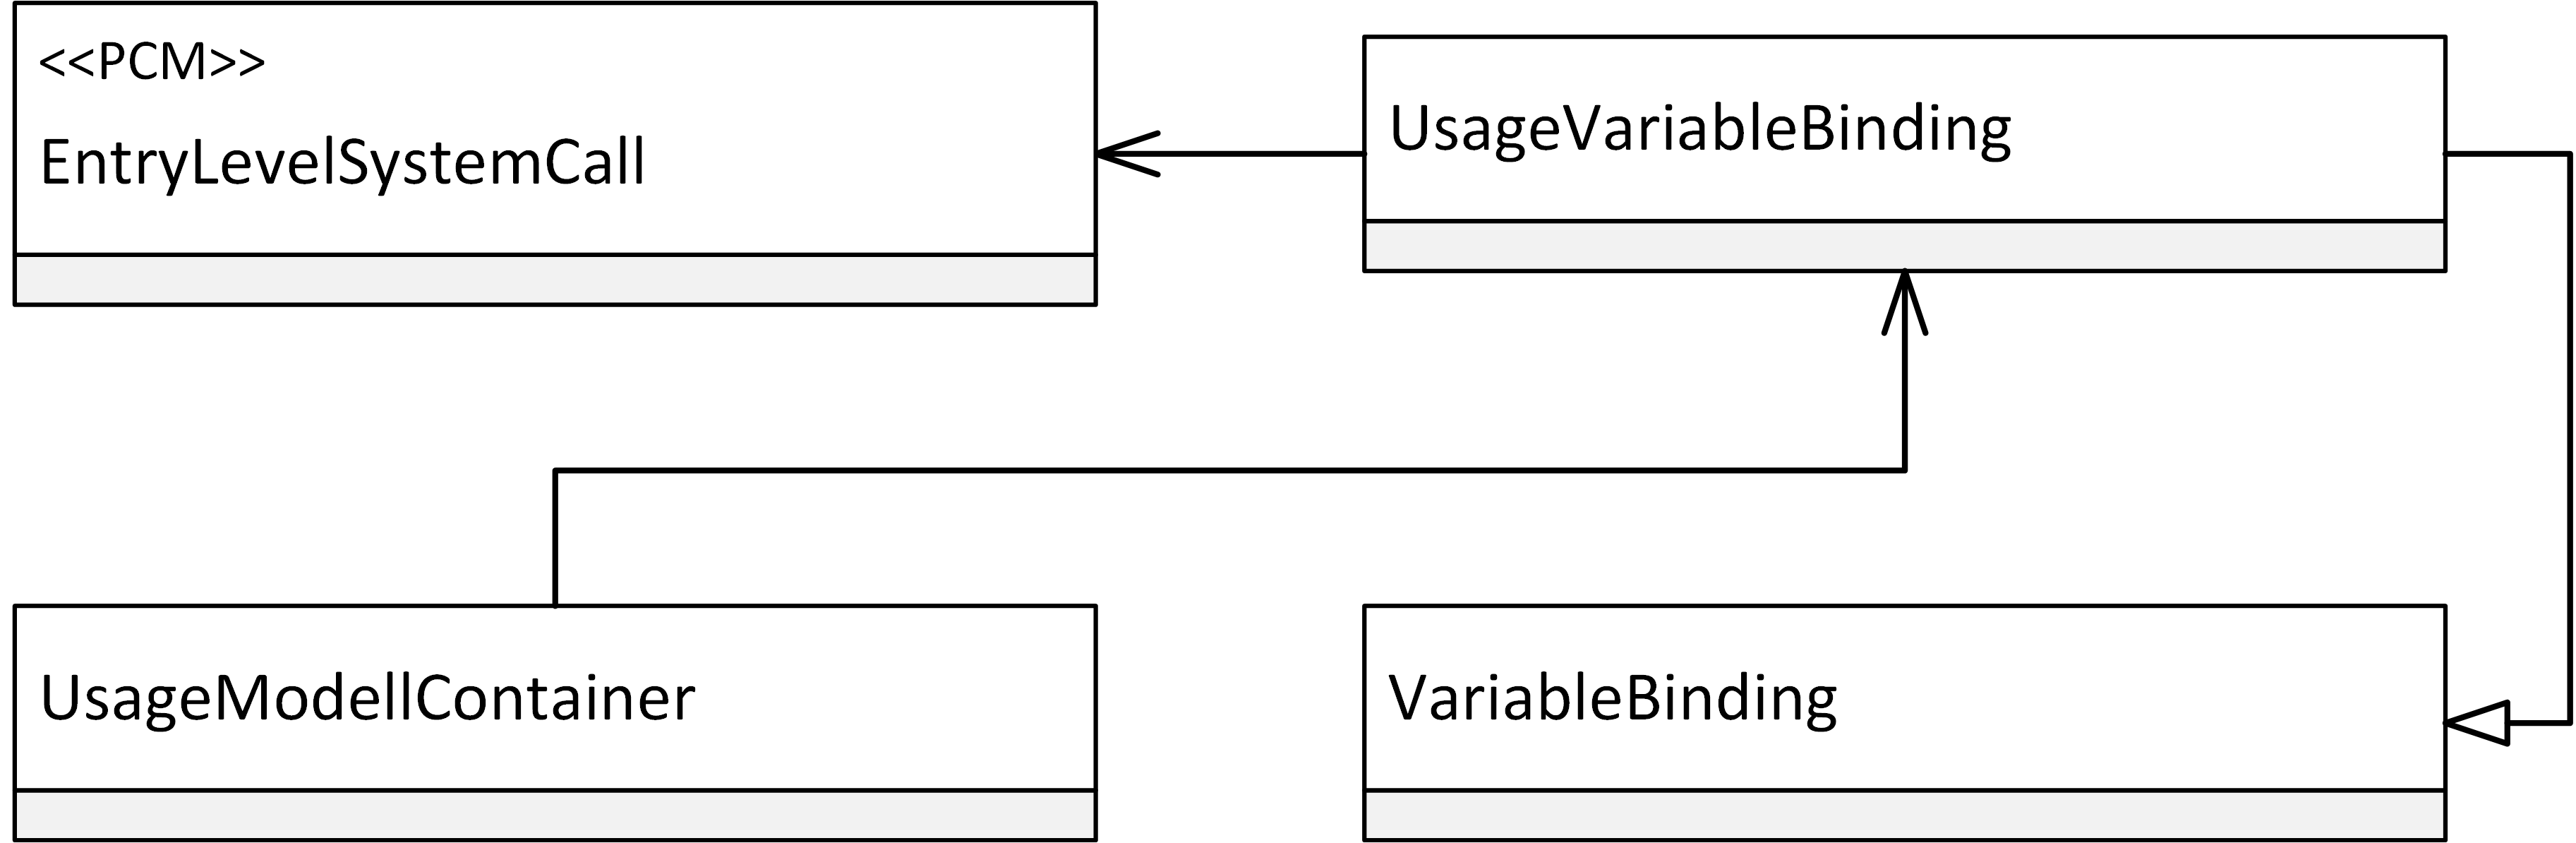
\includegraphics[width=0.85\textwidth]{images/meta_usage.png}
	\caption{Modellierung der Erweiterung für das Nutzungsmodell}
	\label{img:modell:usage}
\end{figure}
In \autoref{img:szenario:usage} ist der Datenfluss im Nutzungsmodell, anhand des Beispiels aus \autoref{sec:szenario}, modelliert. In der Modellierung gibt es die Datenklassen \textit{ProductData} und \textit{CreditCardData}. Der Datenfluss beginnt mit einem \texttt{EntryLevelSystemCall}, der den Dienst \texttt{buy(Product product)} aufruft. Außerdem wird er von einem \texttt{UsageBinding}, dass den Parameter \textit{product} mit der Datenklasse \textit{ProductData} verknüpft, referenziert. Die Daten fließen zum Nächsten \texttt{EntryLevelSystemCall}, welcher wiederum den Dienst \texttt{pay(CreditCard creditCard)} aufruft. Auch dieser \texttt{EntryLevelSystemCall} wird von einem \texttt{UsageBinding}, dass den Paramter \textit{creditCard} mit der Datenklasse \textit{CreditCardData} verknüpft, referenziert. Danach endet der Datenfluss.

\begin{figure}[h]
	\centering
  	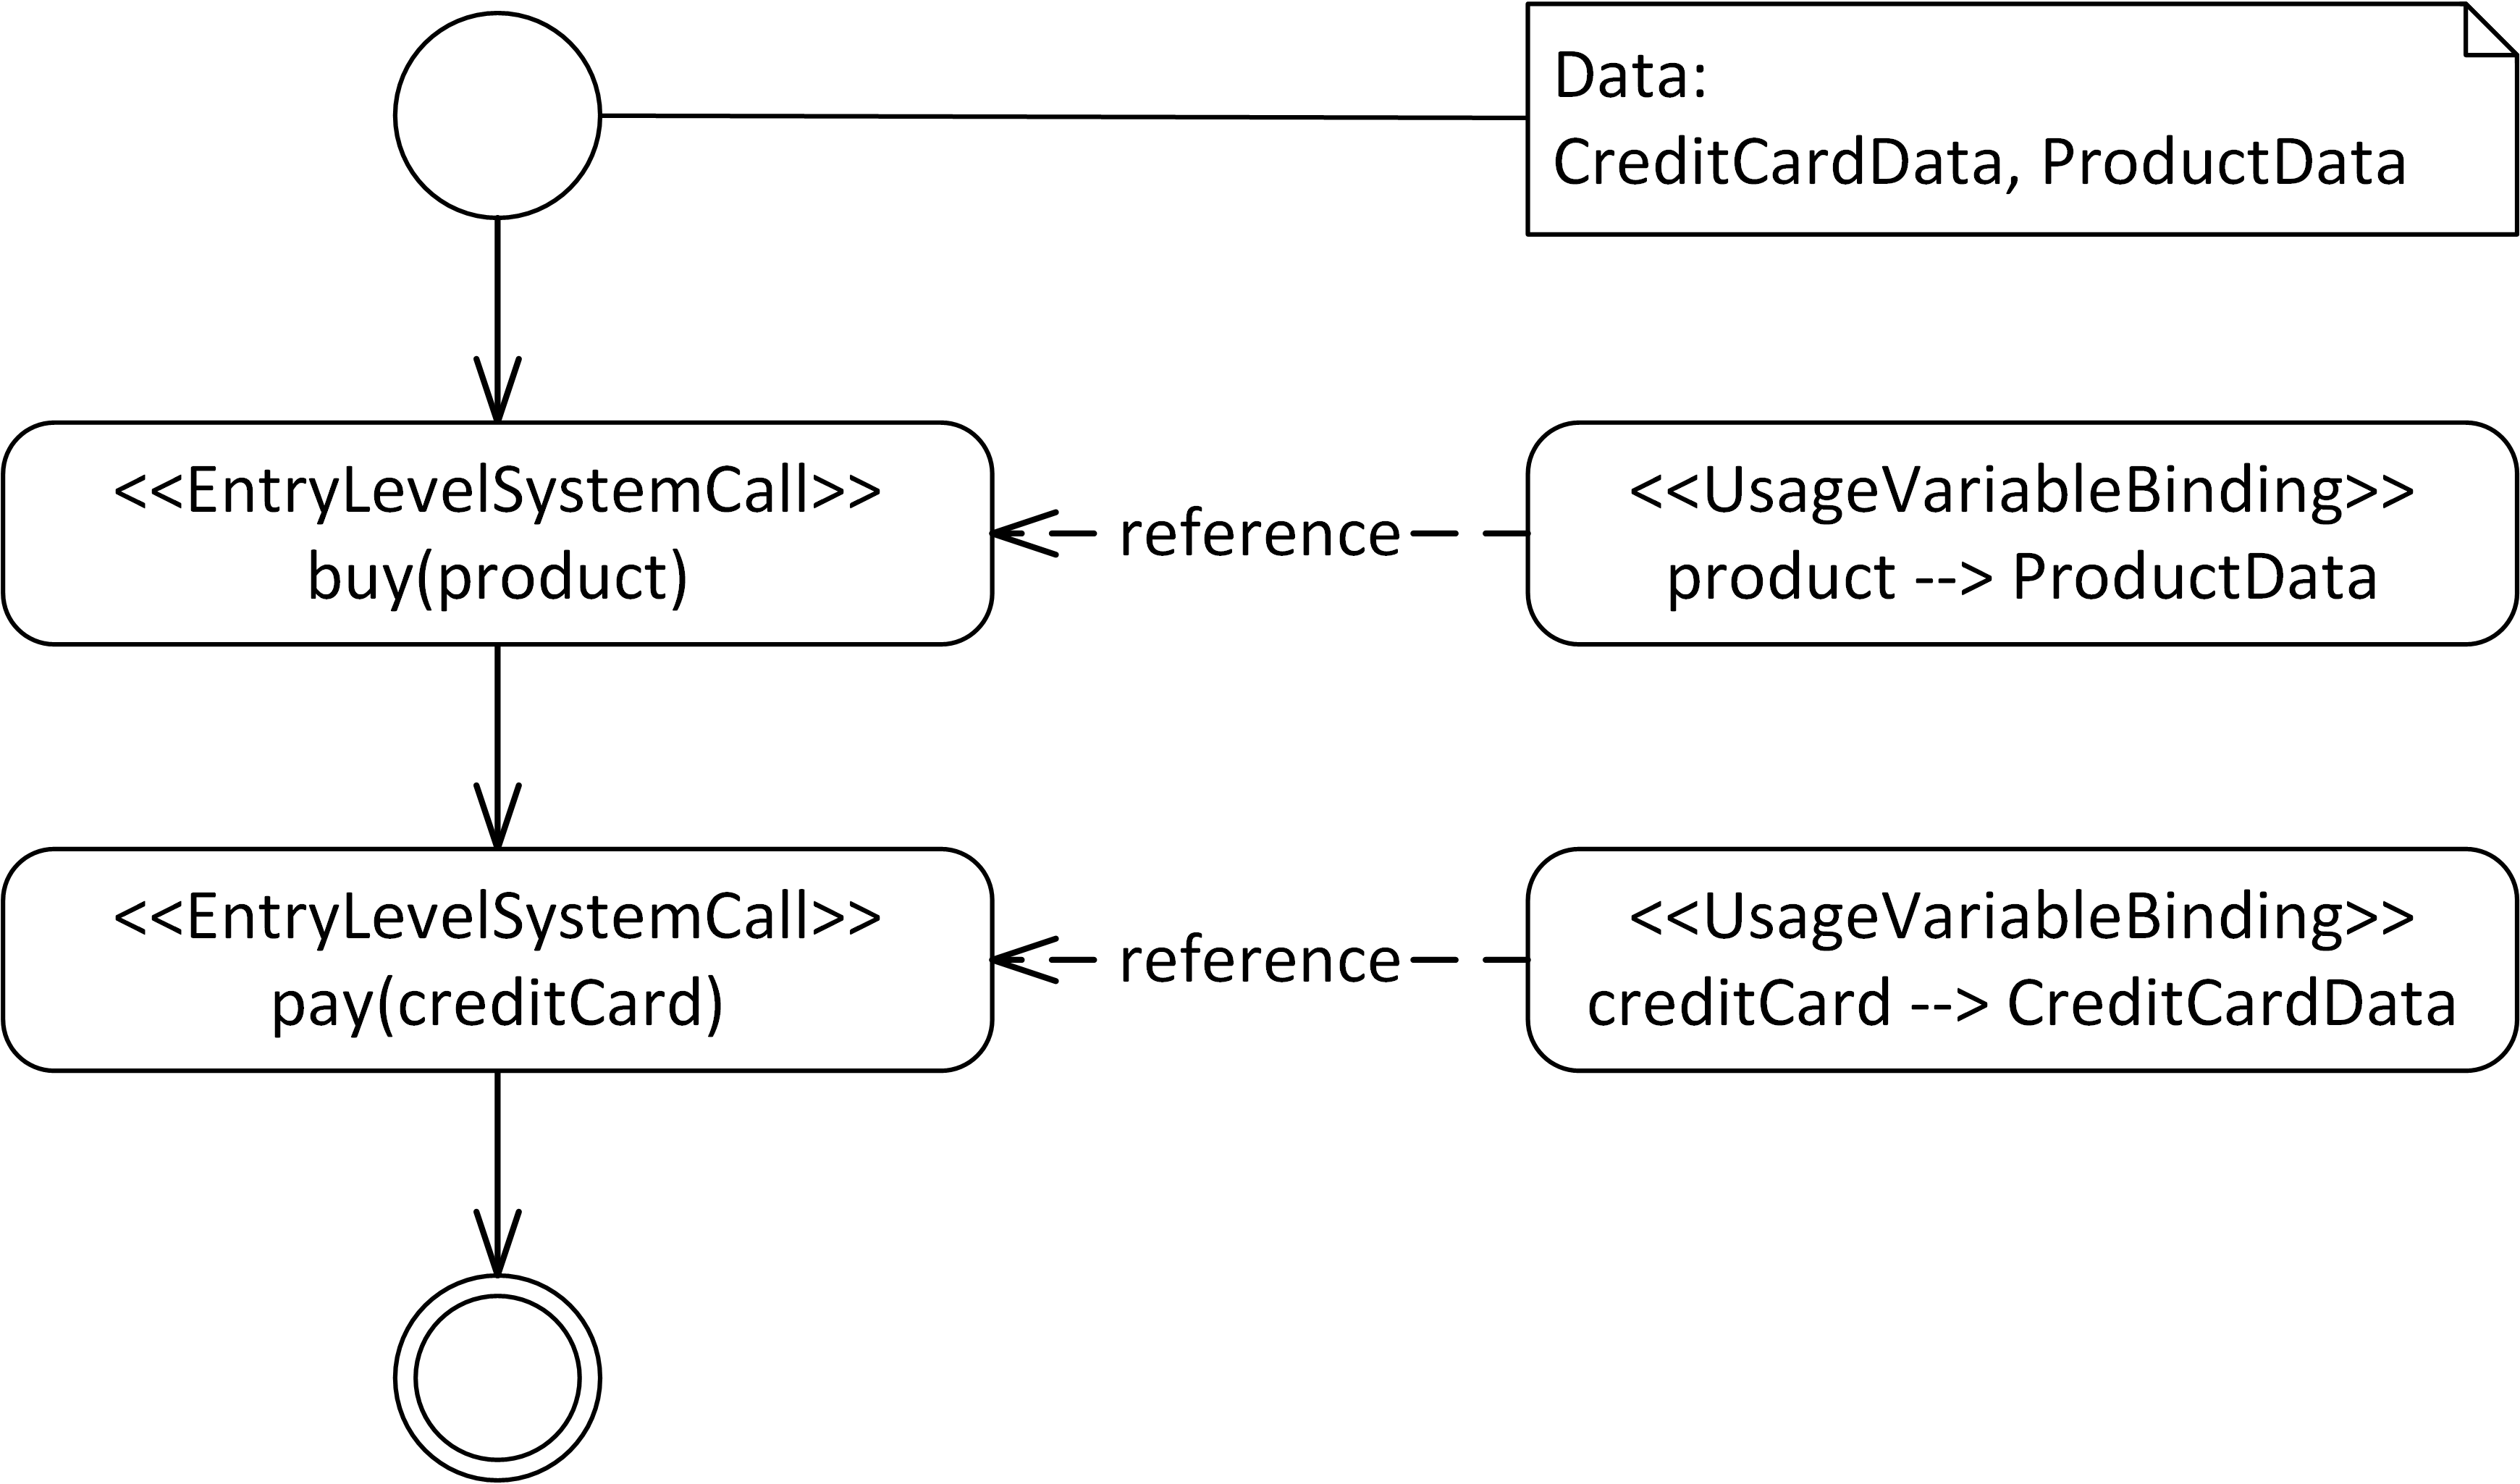
\includegraphics[width=0.85\textwidth]{images/szenario_usage.png}
	\caption{Datenfluss, der vom Benutzer ausgeht}
	\label{img:szenario:usage}
\end{figure}
%%% LaTeX2e class for student theses
%% sections/content.tex
%% 
%% Karlsruhe Institute of Technology
%% Institute for Program Structures and Data Organization
%% Chair for Software Design and Quality (SDQ)
%%
%% Dr.-Ing. Erik Burger
%% burger@kit.edu
%%
%% Version 1.1, 2014-11-21

\chapter{Implementierung}
\label{ch:implementierung}
Evtl in Kapitel Validierung schieben
\section{RC und LR Annotationen}
mithilfe von profiles \\
was sind profiles

\section{SEFF}

\section{Usage-Modell}

%% LaTeX2e class for student theses
%% sections/evaluation.tex
%% 
%% Karlsruhe Institute of Technology
%% Institute for Program Structures and Data Organization
%% Chair for Software Design and Quality (SDQ)
%%
%% Dr.-Ing. Erik Burger
%% burger@kit.edu
%%
%% Version 1.1, 2014-11-21

\chapter{Validierung}
\label{ch:Validierung}
Im Laufe der Bachelorarbeit wird ein Ansatz zu Modellierung von Datenflüssen auf Architekturebene entwickelt.
Um den Nachweis über die Einsatzeignung der entwickelten Methodik aus Abschnitt \ref{ch:Konzeption} zu erbringen, soll geprüft werden ob die Eigenschaften nach Stachowiak (vgl. Kapitel \ref{subch:Modell}) erfüllt sind. Die Eigenschaften \textbf{Abbildung} und \textbf{Verkürzung} sind gegeben, da es sich um eine Abbildung von Datenflüssen handelt und nur relevante Attributen erfasst werden. Schließlich muss die Eigenschaft \textbf{Pragmatismus} geprüft werden. Pragmatismus ist gegeben, wenn die Modelle für ihren späteren Einsatzzweck geeignet sind. Im Rahmen der Bachelorarbeit sind Analysen der Einsatzzweck. Deshalb muss geprüft werden ob das Meta-Modell auch diese Eigenschaft unterstützt. Dafür gibt es zwei Ansätzen.\par
Der erste Ansatz ist die Vertraulichkeitsanalyse aus \cite{Kramera}. Diese Analyse prüft die Vertraulichkeit in komponentenbasierten Systemen. Für die Analyse müssen Eingabe und Ausgabe eines Systems spezifiziert werden, sowie Zugriffsspezifikation für Hardware und Kommunikationsverbindungen. Mithilfe dieser Informationen und einem Angreifer Modell wird eine Architektur- und Code-Analyse durchgeführt. Nach Durchführung der Analyse werden Designfehler, Datenlecks und Verstöße gegen die Spezifikation angezeigt. Die Analyse soll auf einem oder beiden Fallbeispielen aus der Arbeit laufen. Dabei handelt es sich um ein verteiltes Reiseplaner-System und um ein Cloud-Hosting-System mit zwei Tiers. Beide Systeme müssen vor der Analyse mit Datenflüssen ausgestattet werden. Dies geschieht, indem spezifiziert wird, welche Parameter sich innerhalb der Komponente beeinflussen. Für die Validierung muss die Analyse ebenfalls angepasst werden, damit der Datenfluss berücksichtigt wird. \par
Eine weitere Möglichkeit der Validierung kann mithilfe einer anderen Analyse durchgeführt werden. Die Analyse soll über Modellabfragen realisiert werden. Dazu kann zum Beispiel eine Analyse aus der Literatur genommen werden. Als Fallbeispiel soll der Palladio MediaStore \cite{Reussner} dienen, für den davor Datenflüsse modelliert werden.


%% LaTeX2e class for student theses
%% sections/conclusion.tex
%% 
%% Karlsruhe Institute of Technology
%% Institute for Program Structures and Data Organization
%% Chair for Software Design and Quality (SDQ)
%%
%% Dr.-Ing. Erik Burger
%% burger@kit.edu
%%
%% Version 1.1, 2014-11-21

\chapter{Zusammenfassung und Ausblick}
\label{ch:zusammenfassung}

In dieser Bachelorarbeit wurde eine Datenflussdokumentation auf Architekturebene vorgestellt. Mit dieser Datenflussdokumentation ist es möglich Modelle des \gls{pcm} um Daten und Datenflüsse zu erweitern. Die Elemente, mit denen das möglich ist, sind in \autoref{ch:modellierung} beschrieben. In \autoref{ch:validierung} wurde dann mithilfe eines Fallbeispiels gezeigt, dass mit der Modellierung Daten und Datenflüsse modelliert werden können. Dabei ist eine Modellierung von Daten und Datenflüssen, ausgehend vom Benutzer des Systems, zu den Komponenten und innerhalb der Komponenten möglich. Außerdem wurde gezeigt, dass die Modellierung in Datenflussanalysen verwendet werden kann. Dazu wurden die Datenflüsse innerhalb des Modells analysiert und transformiert. Das transformierte Modell wurde verwendet um die Eingabe und Ausgabe des Fallbeispiels zu spezifizieren. Anschließend wurde versucht mithilfe einer Vertraulichkeitsanalyse nach Kramer et. al. \cite{Kramera} diese Modellierung zu überprüfen. Leider konnte diese, aufgrund eines Defekts, nicht vollständig ausgeführt werden. Stattdessen wurden das Vertraulichkeitsmodell und das transformierte Modell verglichen. Die Unterschiede wurden diskutiert und zu dem Ergebnis geführt, dass die Modellierung dieser Bachelorarbeit durchaus für Datenflussanalysen geeignet ist. \par 
Die Datenflussdokumentation, die in dieser Bachelorarbeit entstanden ist, dient dabei die einzelnen Rollen und die dazugehörigen Modelle, des \gls{pcm}, zu erweitern. Sie ermöglicht dem Komponentenentwickler das Verhalten innerhalb von Komponenten um einen Datenfluss zu erweitern. Somit wird das Komponenten-Reposiory-Modell erweitert. Auch dem Domänenexperten wird es ermöglicht Datenflüsse zu modellieren. Die Datenflüsse gehen vom Benutzer aus und erweitern das Nutzungsmodell. Schließlich wird dem Software-Verteilungsexperten ermöglicht eine Hardware-Spezifikation im Ressourcen-Umgebungs-Modell durchzuführen. \par
Für zukünftige Arbeiten könnte die Modellierung dieser Bachelorarbeit mit weiteren Fallbeispielen validiert werden. Indem weitere Fallbeispiele erstellt oder existierende aus der Literatur mit Datenflüssen erweitert werden, könnte die Modellierung genauer validiert werden. Als Beispiel würde sich z.B. das zweite Fallbeispiel aus der Arbeit von Kramer et. al. \cite{Kramera} eignen, da dieses bereits über modellierte PCM-Modelle verfügt. Außerdem könnten weitere Datenflussanalysen betrachtet werden. Dabei könnten andere Sicherheitseigenschaften überprüft werden. Die Datenflussanalyse aus der Arbeit \textbf{UMLsec} \cite{Jurjens2005} könnte sich dazu eignen. Dafür müsste die dortige Modellierung und Analyse betrachtet werden und im Anschluss eine Transformation geschrieben werden, die ein Modell dieser Bachelorarbeit in ein \textbf{UMLsec}-Modell transformiert. Dazu könnten die Fallbeispiele von \textbf{UMLsec} mithilfe des \gls{pcm} nachmodelliert, mit Daten und Datenflüssen erweitert und die jeweiligen Ergebnisse verglichen werden. Um die Modellierung besser in Palladio-Workbench zu integrieren, könnte ein graphischer Editor erstellt werden, mit dem Daten und Datenflüsse erstellt werden können. Damit könnte die Akzeptanz bei den Architekten geprüft werden. Die Masterarbeit \textbf{Flexible Graphical Editors for Extensible Modular Meta Models} von Michael Junker, setzt sich mit dem Thema auseinander, wie sich erweiterbare Meta-Modelle auf flexible graphische Editoren auswirken. Dabei wurde auch die Erweiterung dieser Bachelorarbeit betrachtet. Außerdem wird in einer weiteren Masterarbeit von Philipp Weimann diese Bacheorarbeit auch betrachtet. In der Masterarbeit werden Applikationen untersucht, die verteilt in der Cloud liegen. Auslagerungen sollen dabei automatisch erkannt werden und bei Verstoß gegen vorgegebene Richtlinien eine alternative Verteilung des Systems ermittelt und angewendet werden.





%% --------------------
%% |   Bibliography   |
%% --------------------

%% Add entry to the table of contents for the bibliography
\printbibliography[heading=bibintoc]



%% ----------------
%% |   Appendix   |
%% ----------------
\appendix
%% LaTeX2e class for student theses
%% sections/apendix.tex
%% 
%% Karlsruhe Institute of Technology
%% Institute for Program Structures and Data Organization
%% Chair for Software Design and Quality (SDQ)
%%
%% Dr.-Ing. Erik Burger
%% burger@kit.edu
%%
%% Version 1.1, 2014-11-21


\iflanguage{english}
{\chapter{Appendix}}    % english style
{\chapter{Anhang}}      % german style
\label{chap:appendix}


%% -------------------
%% | Example content |
%% -------------------
\section{First Appendix Section}
\label{sec:appendix:FirstSection}
		
\setcounter{figure}{0}
		
\begin{figure} [ht]
  \centering
  \missingfigure{A figure}
  \caption{A figure}
  \label{fig:anotherfigure}
\end{figure}


\dots
%% ---------------------
%% | / Example content |
%% ---------------------

\end{document}
